\documentclass[12pt,a4paper,openright]{report}

% ---------- Encoding & language ----------
\usepackage[utf8]{inputenc}
\usepackage[T1]{fontenc}
\usepackage[english]{babel}

% ---------- Typography ----------
\usepackage{lmodern}
\usepackage{microtype}
\usepackage{setspace}
\onehalfspacing

% ---------- Layout ----------
\usepackage[a4paper,margin=2.8cm,headheight=15pt]{geometry}
\usepackage{emptypage}

% ---------- Math ----------
\usepackage{amsmath}
\usepackage{amssymb}
\usepackage{amsthm}
\usepackage{mathtools}
\DeclareMathOperator*{\argmin}{arg\,min}

% ---------- Graphics ----------
\usepackage{graphicx}

% ---------- Bibliography ----------
\usepackage[
  backend=biber,
  style=numeric-comp,
  sorting=none,
  maxbibnames=99
]{biblatex}
\addbibresource{references.bib}

% ---------- Lists, tables, code ----------
\usepackage{enumitem}
\setlist{itemsep=2pt, topsep=4pt}
\usepackage{booktabs}
\usepackage{listings}
\lstset{
  basicstyle=\ttfamily\small,
  frame=single,
  breaklines=true,
  showstringspaces=false,
  columns=fullflexible
}
\usepackage{xcolor}

\definecolor{promptbg}{RGB}{248,249,250}
\definecolor{promptframe}{RGB}{206,212,218}
\definecolor{promptrule}{RGB}{74,144,217}

\lstdefinestyle{prompt}{
  basicstyle=\ttfamily\footnotesize,
  backgroundcolor=\color{promptbg},
  frame=single,
  framerule=0.8pt,
  rulecolor=\color{promptframe},
  breaklines=true,
  breakindent=0pt,
  % postbreak=\mbox{\textcolor{promptrule}{$\hookrightarrow$}\space},
  showstringspaces=false,
  columns=fullflexible,
  xleftmargin=10pt,
  xrightmargin=4pt,
  aboveskip=10pt,
  belowskip=10pt,
  captionpos=b,
}


% ---------- Hyperlinks ----------
\usepackage[hidelinks]{hyperref}

% ---------- Headers ----------
\usepackage{fancyhdr}
\pagestyle{fancy}
\fancyhf{}
\fancyhead[L]{\nouppercase{\leftmark}}
\fancyhead[R]{\thepage}
\renewcommand{\headrulewidth}{0.4pt}
\fancypagestyle{plain}{%
  \fancyhf{}%
  \fancyfoot[C]{\thepage}%
  \renewcommand{\headrulewidth}{0pt}%
}

% ---------- Chapter titles ----------
\usepackage{titlesec}
\titleformat{\chapter}[display]
  {\normalfont\sffamily\Huge\bfseries}
  {\chaptertitlename\ \thechapter}{12pt}{\Huge}
\titlespacing*{\chapter}{0pt}{-20pt}{30pt}
\usepackage[titletoc,title]{appendix}

% ---------- Macros ----------
\newcommand{\ie}{\textit{i.e.}}
\newcommand{\eg}{\textit{e.g.}}
\newcommand{\code}[1]{\texttt{#1}}

% ============================================================
\begin{document}

% -------------------------
% TITLE PAGE
% -------------------------
\begin{titlepage}
    \centering
    \vspace*{1cm}
    {\large UNIVERSITAT POLITÈCNICA DE CATALUNYA \\ BARCELONATECH \par}
    \vspace{0.4cm}
    {\large Facultat d'Informàtica de Barcelona (FIB)\par}

    \vspace{3.5cm}

    {\Large\bfseries Generative Graph Databases for Building Structures via Visual Analysis with Large Language Models\par}

    \vspace{2.5cm}

    {\large HANG YAO\par}

    \vspace{2cm}

    \begin{center}
        \textbf{Thesis director:} \\
        Enrique Romero Merino (Department of Computer Architecture)

        \vspace{0.6cm}
        
        \textbf{Thesis co-director:} \\
        Lluís Ortega Cerdà (Department of Architectural Design)
    \end{center}

    \vfill

    {\large Master's Degree in Data Science\par}
    \vspace{0.4cm}
    {\large Master's Thesis\par}
    \vspace{0.4cm}
    {\large Facultat d'Informàtica de Barcelona (FIB)\\
            Universitat Politècnica de Catalunya \textendash{} BarcelonaTech\par}
    \vspace{0.6cm}
    {\large \today\par}
\end{titlepage}

% -------------------------
% ABSTRACT
% -------------------------
\pagenumbering{arabic}
\setcounter{page}{1}

\chapter*{Abstract}
\addcontentsline{toc}{chapter}{Abstract}

The architectural domain relies heavily on the manual analysis of 2D floor plans, a process that is time-consuming, costly, and prone to inconsistency between annotators. While the visual verification of spatial correctness still requires a human expert, modern \textbf{Vision-Language Models (VLMs)} offer a credible pathway to automate the structural extraction that precedes it.

This thesis proposes an end-to-end pipeline that converts raster floor-plan images into structured 2D and 3D topological graphs using a locally hosted VLM (\textbf{Qwen3-VL}). The system decomposes the extraction problem into six focused sub-tasks --- classification, aggregation analysis, apartment detailing, graph assembly, human-in-the-loop refinement, and 3D alignment --- each driven by a carefully engineered prompt that combines an architect's profile, strong-signal enumeration, ordered decision procedures, and one-shot visual examples. A deterministic algorithm subsequently aligns vertical circulation elements (staircases and elevators) across floors to produce a cohesive 3D building representation.

The pipeline is applied to a corpus of \textit{1,276} social-housing plans from three \textbf{Catalan institutional datasets} (IBAVI, IMPSOL, INCASOL). Since no ground-truth annotations exist for these datasets, validation rests on two complementary criteria: deterministic structural checks on the extracted graphs, and manual spot-checking against the source images. The resulting graph database is designed to feed downstream generative models capable of producing structurally valid residential layouts.

\medskip
\noindent\textbf{Keywords:} Vision-Language Models, floor-plan analysis, architectural graphs, prompt engineering, social housing, in-context learning, human-feedback

% -------------------------
% TABLE OF CONTENTS
% -------------------------
\newpage
\renewcommand{\contentsname}{Contents}
\tableofcontents

% ============================================================
\newpage

\chapter{Introduction}

\section{Motivation}
\label{sec:motivation}

Residential architecture is a highly data-rich discipline: every housing project generates dozens of technical drawings, floor plans, and graphic catalogues that capture decades of accumulated design knowledge. In the specific context of Catalan public housing---promoted by agencies such as \textbf{IBAVI} (\textit{Institut Balear de l'Habitatge}), \textbf{IMPSOL} (\textit{Institut Metropolità de Promoció de Sòl}), and \textbf{INCASOL} (\textit{Institut Català del Sòl})---this knowledge is dispersed across thousands of archival floor plans whose typological consistency makes them an ideal substrate for data-driven research.

Despite the sheer volume of available material, this historical data remains effectively locked inside static raster images. Existing computer-aided design (CAD) tools require manual interpretation, and modern data-hungry generative models cannot consume raw JPG or PNG drawings directly; they require structured, machine-readable descriptions of rooms, dimensions, and topology. Producing these annotations by hand is prohibitively expensive---a single complex floor plan can take an experienced architect between ten and twenty minutes to label fully---and inherently prone to inconsistencies across different human annotators.

The recent maturation of Vision-Language Models (VLMs) offers a paradigm shift for this bottleneck. Open-weights architectures such as Qwen3-VL~\cite{bai2023qwenvlversatilevisionlanguagemodel}, LLaVA~\cite{liu2023llava}, and InternVL~\cite{chen2024internvlscalingvisionfoundation} now combine reliable optical character recognition (OCR) with robust spatial reasoning. This makes it plausible to extract architectural semantics directly from an image through structured natural-language prompting. This thesis investigates whether such an automated workflow can reliably replace manual annotation for social housing datasets, establishing a scalable pipeline to unlock this architectural heritage.

The conceptual foundation for this approach was originally inspired by methodologies such as Pred-LLM~\cite{nguyen2024generatingrealistictabulardata}, which successfully demonstrated the capacity of Large Language Models to generate and structure realistic tabular data. Translating this premise to the architectural domain prompted a novel research question: if language models can infer structured tabular schemas, could their multimodal counterparts (VLMs) reliably extract and map complex, multi-relational spatial graphs from visual inputs? This theoretical leap shaped the core objective of this work: to transform static floor plans into structured topological graphs, thereby laying the essential groundwork for future generative AI models in building design.

\section{Objectives}

The primary objective of this thesis is to design, implement, and validate an automated, end-to-end pipeline capable of extracting structured 2D architectural graphs from unannotated raster floor plans of Catalan social housing (e.g., IBAVI, IMPSOL, INCASOL). Utilizing a locally hosted Vision-Language Model (VLM), the system is engineered to translate unstructured visual layouts into formalized topological data (apartments and structural connections), thereby generating a robust dataset of residential topologies to serve as foundational training data for future generative architectural models.

To achieve this overarching goal, the research is decomposed into the following specific, verifiable sub-objectives:

\begin{enumerate}
    \item \textbf{VLM Infrastructure and Deterministic Classification:} Build a reproducible inference framework wrapping a localized VLM (e.g., Qwen3-VL) optimized for constrained hardware. This includes engineering a deterministic classification mechanism utilizing greedy decoding to accurately categorize floor plans into three classes: aggregated residential floors, individual dwellings, and non-residential plans (\textit{other}).
    
    \item \textbf{Few-Shot Visual Prompting Architecture:} Design a multi-stage, persona-driven prompt strategy that employs canonical one-shot and two-shot visual reference examples. This approach decomposes the topological extraction process into focused sub-tasks---classification, aggregation analysis, and apartment-level detailing---to systematically minimize visual hallucination.
    
    \item \textbf{Topological Graph Assembly:} Translate the sequentially extracted visual features into formalized 2D graph structures (encoded via \textit{JSON} and \textit{NetworkX}), where nodes denote discrete apartments and shared circulation elements (e.g., staircases, elevators) --- with each apartment's interior room inventory carried as node attributes --- and edges represent physical spatial connections.
    
    \item \textbf{Persistent Visual Memory (HITL):} Implement a human-in-the-loop (HITL) correction mechanism that captures expert architectural feedback. This system will extract reference crops of complex architectural elements and persist them as a dynamic, few-shot visual memory buffer across inference sessions, allowing the model to adapt without requiring weight-level retraining.
    
    \item \textbf{Annotation-Free Validation Strategy:} Formulate and apply an annotation-free validation framework. By enforcing deterministic structural checks on each graph and complementing them with manual spot-checks, the system evaluates the generated topologies without relying on manual ground-truth datasets, which are unavailable for the target architectural corpora.
\end{enumerate}


\section{Scope}

The scope of this research is strictly bounded to Catalan social-housing floor plans sourced from three institutional datasets (IBAVI, IMPSOL, INCASOL), corresponding to 1,276 raster images. Plans involving non-residential typologies, exterior site drawings, and pure elevations are explicitly filtered out during preprocessing.

The chosen Vision-Language Model is Qwen3-VL (specifically the 8B Instruct variant~\cite{qwen3technicalreport}). This model was selected for its open weights, native multi-image input processing---which is mandatory for few-shot visual prompting---and its state-of-the-art performance on document-understanding benchmarks. This latter capability is highly relevant given the density of architectural text abbreviations on social-housing plans. The model is executed locally and remains completely frozen. All engineering efforts are concentrated entirely on persona-driven prompt design, dynamic in-context visual examples, and pipeline orchestration. This constraint ensures the research remains fully reproducible on standard commodity hardware (e.g., an NVIDIA A5000 GPU for full-dataset inference) while bypassing the financial costs and algorithmic opacity associated with commercial cloud APIs.

The proposed pipeline produces two primary artifacts: (i) structured, per-image 2D architectural graphs in JSON format, capturing room-level semantics and intra-floor topological connections; and (ii) per-building 3D spatial graphs that systematically align the individual 2D floor representations via shared vertical circulation nodes. The downstream generation of novel floor plans utilizing this extracted dataset is explicitly outside the scope of this thesis. Such generative applications are reserved for future work, as they necessitate dedicated generative modeling strategies, including full-parameter fine-tuning or advanced few-shot prompting techniques to conditionally generate valid architectural JSON structures.

\section{Document Structure}

The remainder of this thesis is organized as follows:
\begin{itemize}
    \item \textbf{Chapter~\ref{ch:background}} reviews the relevant state of the art, covering traditional floor-plan analysis, multi-modal language models, in-context learning strategies, and graph-theoretic representations in architecture, and surveys recent related work applying vision-language models to floor plans (Section~\ref{sec:related-work}), positioning this thesis as an annotation-free, prompting-only alternative to the current fine-tuned approaches.
    \item \textbf{Chapter~\ref{ch:problem}} formalizes the problem of unstructured visual data in social housing and presents the high-level system architecture designed to address it.
    \item \textbf{Chapter~\ref{ch:methodology}} details the core methodological contributions, including the deterministic classification strategy, the multi-step 2D extraction prompts, the Human-in-the-Loop (HITL) persistent visual memory, and the deterministic algorithms utilized for 3D vertical alignment.
    \item \textbf{Chapter~\ref{ch:implementation}} documents the technical implementation of the VLM inference wrapper and the dataset processing pipeline.
    \item \textbf{Chapter~\ref{ch:experiments}} reports the experimental setup, detailing the validation framework (deterministic structural checks and manual spot-checks) and the statistical results of both the 2D extraction and 3D graph generation.
    \item \textbf{Chapter~\ref{ch:discussion}} analyzes the successes of the proposed pipeline while critically examining its limitations, particularly regarding visual hallucinations on dense blueprints.
    \item \textbf{Chapter~\ref{ch:conclusion}} concludes the document with a summary of the technical contributions and outlines specific directions for future research.
\end{itemize}

% ============================================================
\chapter{Background \& State of the Art}
\label{ch:background}

\section{Traditional Floor Plan Analysis}

Computer-based interpretation of floor plans is a problem with a forty-year history. Early systems in the 1980s and 1990s focused on raster-to-vector conversion of CAD drawings, relying on heuristics such as \textbf{Hough transforms} to recover walls, doors, and dimensions~\cite{ahmedFloorPlan2011}. These methods worked well on uniformly drafted technical drawings but degraded sharply on scanned, hand-drawn, or stylised plans.

The advent of convolutional neural networks shifted the field towards data-driven approaches. Liu et al.~\cite{liuRaster2Vec2017} introduced \textbf{Raster2Vec}, an end-to-end CNN that directly predicts a vector representation of walls and openings. Subsequent works such as \textbf{CubiCasa5K}~\cite{kalervo2019cubicasa5kdatasetimprovedmultitask} and the \textbf{DeepFloorPlan} family~\cite{zeng2019deepfloorplanrecognition} expanded the taxonomy to include room semantics and furniture, achieving room-level pixel accuracies above 80\% on curated benchmarks.

These approaches share three limitations that motivate the present work. First, they require sizable annotated datasets to generalise across visual styles --- a resource that does not exist for Catalan social-housing plans. Second, they output dense pixel masks rather than relational structures: the question \textit{``is the kitchen connected to the living room?''} requires an additional post-processing step. Third, they cannot exploit textual cues such as room labels (\textit{H1}, \textit{EMC}, \textit{cuina}) that are abundant in the source material.

\section{Vision-Language Models}

Multi-modal large language models combine a vision encoder with a transformer language model, enabling joint reasoning over images and text. The first notable open-weight family, \textbf{LLaVA}~\cite{liu2023llava}, demonstrated that a relatively small adapter between a \textbf{CLIP}~\cite{radford2021learningtransferablevisualmodels} image encoder and a \textbf{Vicuna}~\cite{vicuna2023} language model could produce coherent visual question answering. Subsequent architectures---\textbf{BLIP-2}~\cite{li2023blip2bootstrappinglanguageimagepretraining}, \textbf{InternVL}~\cite{chen2024internvlscalingvisionfoundation}, \textbf{Qwen-VL}~\cite{bai2023qwenvlversatilevisionlanguagemodel}---progressively improved visual grounding, optical character recognition, and instruction-following.

The Qwen3-VL family~\cite{qwen3technicalreport}, released in 2025, is particularly relevant to the present work. It natively supports interleaved contexts of up to 256K tokens, seamlessly integrating text, images, and video. The 8B Instruct variant fits comfortably in 16\,GB of GPU memory using \code{bfloat16} precision, which makes it deployable on common research hardware.

\section{Prompt Engineering and In-Context Learning}

Without fine-tuning, the behaviour of a VLM is governed entirely by the prompt. The literature on prompt engineering has identified several techniques that are directly applicable to architectural extraction.

\paragraph{Role conditioning.} Giving the model in a specific role (\eg, \textit{``you are a professional architect specialised in Catalan social housing''}) has been shown to reduce hallucination on specialised vocabulary~\cite{kong2024betterzeroshotreasoningroleplay}. The persona biases the language model towards the appropriate sub-distribution of its training corpus.

\paragraph{Decision procedures.} Decomposing a decision into an explicit ordered checklist---\textit{``first count kitchens, then count bathrooms\ldots''}---emulates the chain-of-thought paradigm~\cite{wei2023chainofthoughtpromptingelicitsreasoning} and reduces premature commitment to incorrect answers.

\paragraph{Few-shot and in-context learning.} Prepending one or several reference examples (input + expected output) to the actual query emulates supervised fine-tuning at inference time~\cite{brown2020languagemodelsfewshotlearners}. For multi-modal models, the examples can be images with accompanying descriptions, a regime sometimes called \textit{visual in-context learning}~\cite{bai2023sequentialmodelingenablesscalable}. This thesis exploits both textual and visual in-context examples to teach the model the visual taxonomy of Catalan social housing.

\paragraph{Deterministic decoding.} For classification tasks with a small, fixed answer set, sampling-based decoding introduces unnecessary noise. Greedy decoding (\code{do\_sample} = \textit{False}) eliminates this noise and makes the partition fully reproducible across runs, an essential property for downstream reliability analysis.

\section{Graph Representations for Architecture}
\label{sec:graph_representations}

A floor plan can be naturally encoded as a spatial graph $G = (V, E)$, where vertices ($V$) represent individual spatial units (e.g., apartments, staircases, elevators) and edges ($E$) represent physical adjacency or topological connectivity. This formulation dates back to Hillier's Space Syntax theory~\cite{hillierSpaceSyntax1984} and remains the standard intermediate representation in computational architectural design.

Two primary graph variants are relevant to floor plan analysis: the \textit{adjacency graph} and the \textit{access graph} (illustrated in Figure~\ref{fig:graph-variants}). The adjacency graph encodes all shared physical walls, resulting in a dense, heavily interconnected network. In contrast, the access graph encodes only door- and opening-mediated connections. Because it explicitly maps functional human circulation rather than mere geometric proximity, the access graph accurately captures how inhabitants actually traverse the building. Consequently, it is significantly more informative for generative modeling and is the specific representation adopted in this thesis.

\begin{figure}[ht]
    \centering
    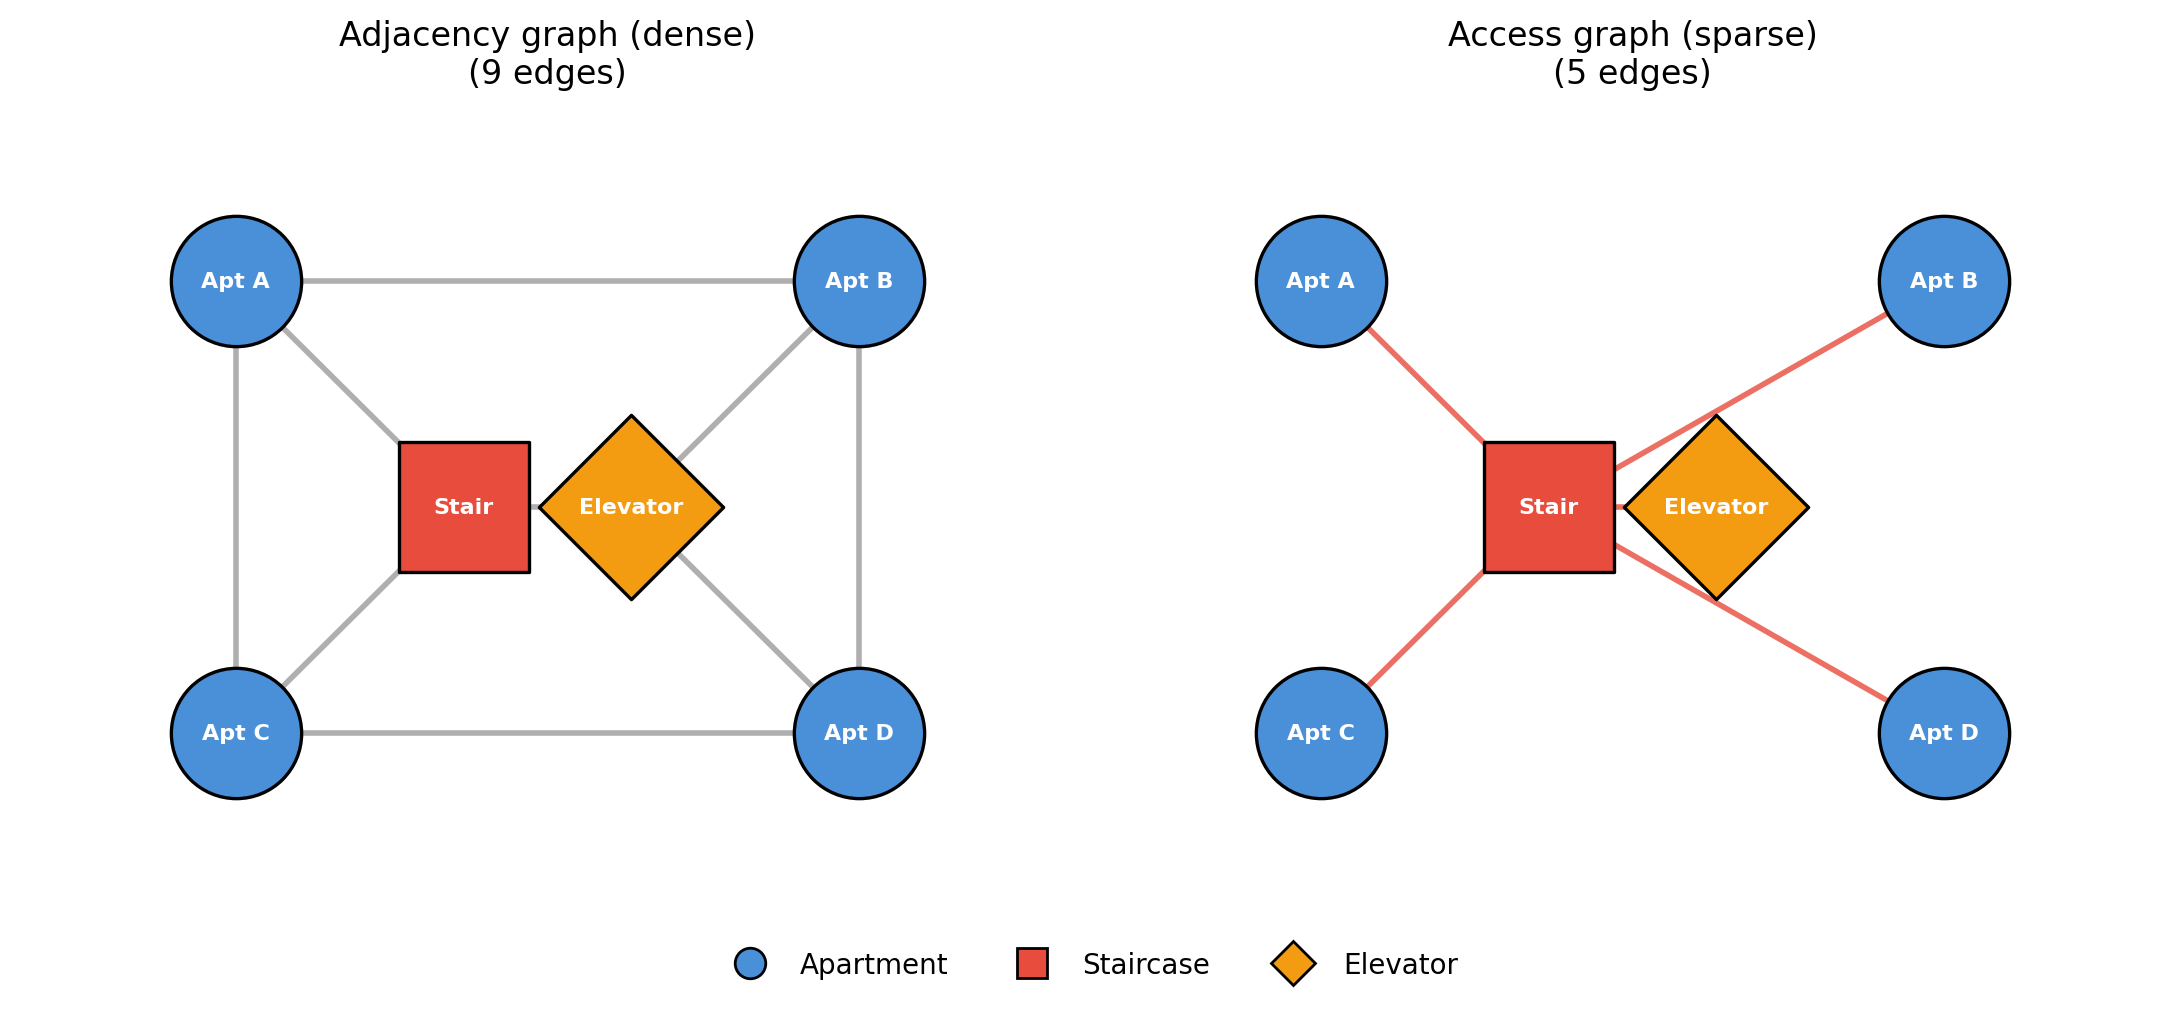
\includegraphics[width=1\textwidth]{figures/graph_variants.png}
    \caption{Comparison of graph encodings for a single residential building floor. Nodes represent individual apartments and shared vertical circulation elements (staircases, elevators). \emph{Left:} The adjacency graph, which forms a dense network by drawing an edge between any two units sharing a physical wall. \emph{Right:} The access graph adopted in this thesis. It forms a sparse, hub-and-spoke topology connecting apartments exclusively to the circulation cores via doors and shared landings, prohibiting direct apartment-to-apartment links to reflect true architectural traversal.}
    \label{fig:graph-variants}
\end{figure}

Generative models for architectural layouts generally fall into two methodological families. The first family operates directly on raster bitmaps using Generative Adversarial Networks (GANs)~\cite{nauata2021housegangenerativeadversariallayout} or diffusion models. While these produce visually plausible floor plans, they offer no mathematical guarantees of structural or functional validity (e.g., they frequently generate enclosed rooms with no doors). The second family operates on graphs using Graph Neural Networks (GNNs) or transformer-based architectures~\cite{nauata2020houseganrelationalgenerativeadversarial}. These models take a strict topological graph as an input constraint and synthesize the corresponding geometric layout around it. The structured access graphs produced by the extraction pipeline in this thesis are explicitly designed to serve as high-fidelity training data for this second, more rigorous family of generative models.

\section{Related Work}
\label{sec:related-work}

The intersection of multimodal models and floor-plan understanding has become an active research area. Existing approaches can be grouped into three threads, against which the present thesis is positioned.

\paragraph{Multimodal models that vectorise or generate plans (trained).} A first line of work fine-tunes or reinforcement-trains multimodal models to reconstruct or synthesise plans. \textit{FloorplanVLM}~\cite{floorplanvlm2026} casts vectorisation as image-conditioned sequence modelling, transcribing rasters into geometric vector code through \texttt{Supervised Fine-Tuning} followed by \texttt{Group Relative Policy Optimisation}. \textit{HouseMind}~\cite{housemind2026} unifies plan understanding, generation, and editing in a single multimodal LLM by discretising layouts into room-instance tokens with a VQ-VAE and instruction-tuning the model. Both achieve strong geometric and topological fidelity, but both depend on large annotated corpora and a dedicated training stage.

\paragraph{Multimodal models that analyse plans (prompting-based).} A second, closer line uses pre-trained models without task-specific training. Recent studies show that VLMs can parse floor-plan maps and identify structural items under zero- and few-shot prompting~\cite{vlmparsefloorplan2025}, and a DocEng case study evaluates visual LLMs for graphics understanding on floor-plan images~\cite{villmsgraphics2025}. \textit{ViLLA}~\cite{villa2025} similarly applies a vision-language analyzer to floor-plan layout. These works share the present method's prompting paradigm, but target object detection or layout description rather than the relational access graph required for generative modelling, and are not specialised to social-housing conventions.

\paragraph{Residential data under scarcity, and embedding-based analysis.} A third thread addresses the same underlying motivation---the scarcity of structured residential data---from a different angle. \textit{Synthetic Homes}~\cite{eshbaugh2026synthetichomes} \emph{generates} multimodal residential building data with generative AI to bypass data-collection barriers, whereas the present work \emph{extracts} structured data from existing plans. Embedding-based methods such as CLIP applied to Korean apartment plans~\cite{clipkorean2026} analyse residential layouts in the same domain (residential apartment plans) but produce similarity embeddings rather than explicit graphs.

\paragraph{Positioning and the choice of prompting over fine-tuning.} This thesis is situated within the prompting-based thread, but differs from all of the above in combining three properties no single prior work provides: it extracts a \emph{topological access graph} (not pixel masks, vector geometry, or embeddings), from \emph{unannotated} Catalan social-housing plans, using a \emph{frozen} VLM driven by prompting alone. The decisive factor in this design is the \textbf{absence of ground-truth annotations} for the IBAVI, IMPSOL, and INCASOL corpora. Fine-tuning and reinforcement-trained approaches such as FloorplanVLM and HouseMind are only viable where a large labelled dataset already exists; for these datasets neither holds, and producing annotations by hand is prohibitively expensive (Section~\ref{sec:problem}). Prompting a pre-trained VLM sidesteps this requirement entirely: the model's general visual-textual competence is driven toward the architectural task through role conditioning, ordered decision procedures, and in-context visual examples, with no parameter updates and therefore no labelled training set. The trade-off is that quality cannot be optimised against a loss on annotated data; the thesis instead controls it through prompt engineering and validates the output through deterministic structural checks and manual spot-checking against the source images (Section~\ref{sec:validation}). Thus, the present work does not merely extend a single prior study; rather, it occupies an unexplored point in the research landscape: annotation-free, prompting-only topological extraction. Ultimately, the pipeline produces the exact structured graphs required to feed and train the downstream generative models discussed above.


% ============================================================
\chapter{Problem Statement \& System Architecture}
\label{ch:problem}

\section{The Problem}
\label{sec:problem}

Given a dataset of $N = 1,276$ raster floor-plan images from three Catalan social-housing programmes, we wish to obtain, for each image, a structured representation suitable for downstream generative modelling. Formally, we seek a function
\[
    \phi : \mathcal{I} \longrightarrow \mathcal{G},
\]
that maps an image $I \in \mathcal{I}$ to a graph $G \in \mathcal{G}$, where $\mathcal{G}$ is the space of architectural graphs whose nodes carry a type label (apartment, staircase, elevator) and whose edges denote physical accessibility.

Three properties of the problem make it non-trivial.

\begin{enumerate}
    \item \textbf{Heterogeneous content.} A non-negligible fraction of the images correspond to \textit{aggregation} plans (a full building floor showing several apartments around shared circulation); others are \textit{individual} plans of a single dwelling; and a further subset are \textit{other} plans that are not habitable dwellings at all (offices, commercial locales, lobbies, parking, technical or pure-circulation floors). These categories require distinct handling---only aggregation plans carry a multi-unit graph to extract---and must be disambiguated automatically.
    \item \textbf{Visual diversity.} Plans vary in style (colour-filled, monochrome, CAD-rendered, hand-drawn), scale, and language of annotation (mostly Catalan). Classical computer-vision techniques struggle with this variability.
    \item \textbf{Absence of ground truth.} No previous annotation effort exists for these datasets, excluding supervised learning and forcing a validation strategy based on deterministic structural checks and manual spot-checks (Section~\ref{sec:validation}).
\end{enumerate}

\section{Design Principles}
\label{sec:principles}

To ensure the extraction pipeline remains robust, reproducible, and resistant to hallucination, four core design principles guide every subsequent engineering decision:

\begin{description}
    \item[Task Decomposition.] The extraction process is strictly modularized. No single Vision-Language Model (VLM) inference step attempts to parse the complete topological graph simultaneously. Instead, prompts are sequentially engineered so that the model evaluates a single, well-bounded architectural decision at a time (e.g., macro-scale building classification followed by micro-scale room inventory extraction).
    
    \item[Domain Anchoring.] Every prompt initializes with an expert architectural persona and embeds a localized Catalan abbreviation dictionary (e.g., \textit{H}, \textit{EMC}, \textit{cuina}). This constraint forces the model to operate within the specific semantic subspace required to correctly interpret regional social-housing conventions.
    
    \item[Deterministic Execution.] To maximize scientific reproducibility, rigid tasks such as the closed-set classification step utilize greedy decoding mechanisms (i.e., enforcing zero temperature and eliminating probabilistic sampling). Probabilistic generation is strictly reserved for complex, open-ended topological extraction where absolute deterministic constraints would degrade the model's spatial reasoning capacity.
    
    \item[Diagnostic Preservation and Fault Tolerance.] Outputs that fail at any stage of the pipeline are not immediately discarded; instead, the pipeline routes data based on a strict two-tier failure taxonomy:
    \begin{itemize}
        \item \textbf{Topological Failures:} Graphs that successfully parse as JSON but fail spatial logic checks (e.g., missing or unreachable vertical circulation) are preserved. They are archived with specific diagnostic flags and routed directly to the Human-in-the-Loop (HITL) step for interactive visual refinement.
        \item \textbf{Extraction Failures:} Instances where the vision-language model fails outright---producing a hallucinated format or no parseable JSON graph---are isolated. Because no spatial topology exists for a human to refine, these cases entirely bypass the interactive review loop and are reserved strictly for final quantitative error reporting.
    \end{itemize}

\end{description}


\section{The Proposed Pipeline}

The system architecture consists of a six-stage pipeline that systematically decomposes the visual extraction function, denoted as $\phi$, into focused, modular sub-tasks. These sub-tasks are executed by a localized Vision-Language Model (VLM) utilizing tailored, stage-specific prompt architectures (Figure \ref{fig:pipeline}).

\begin{figure}
    \centering
    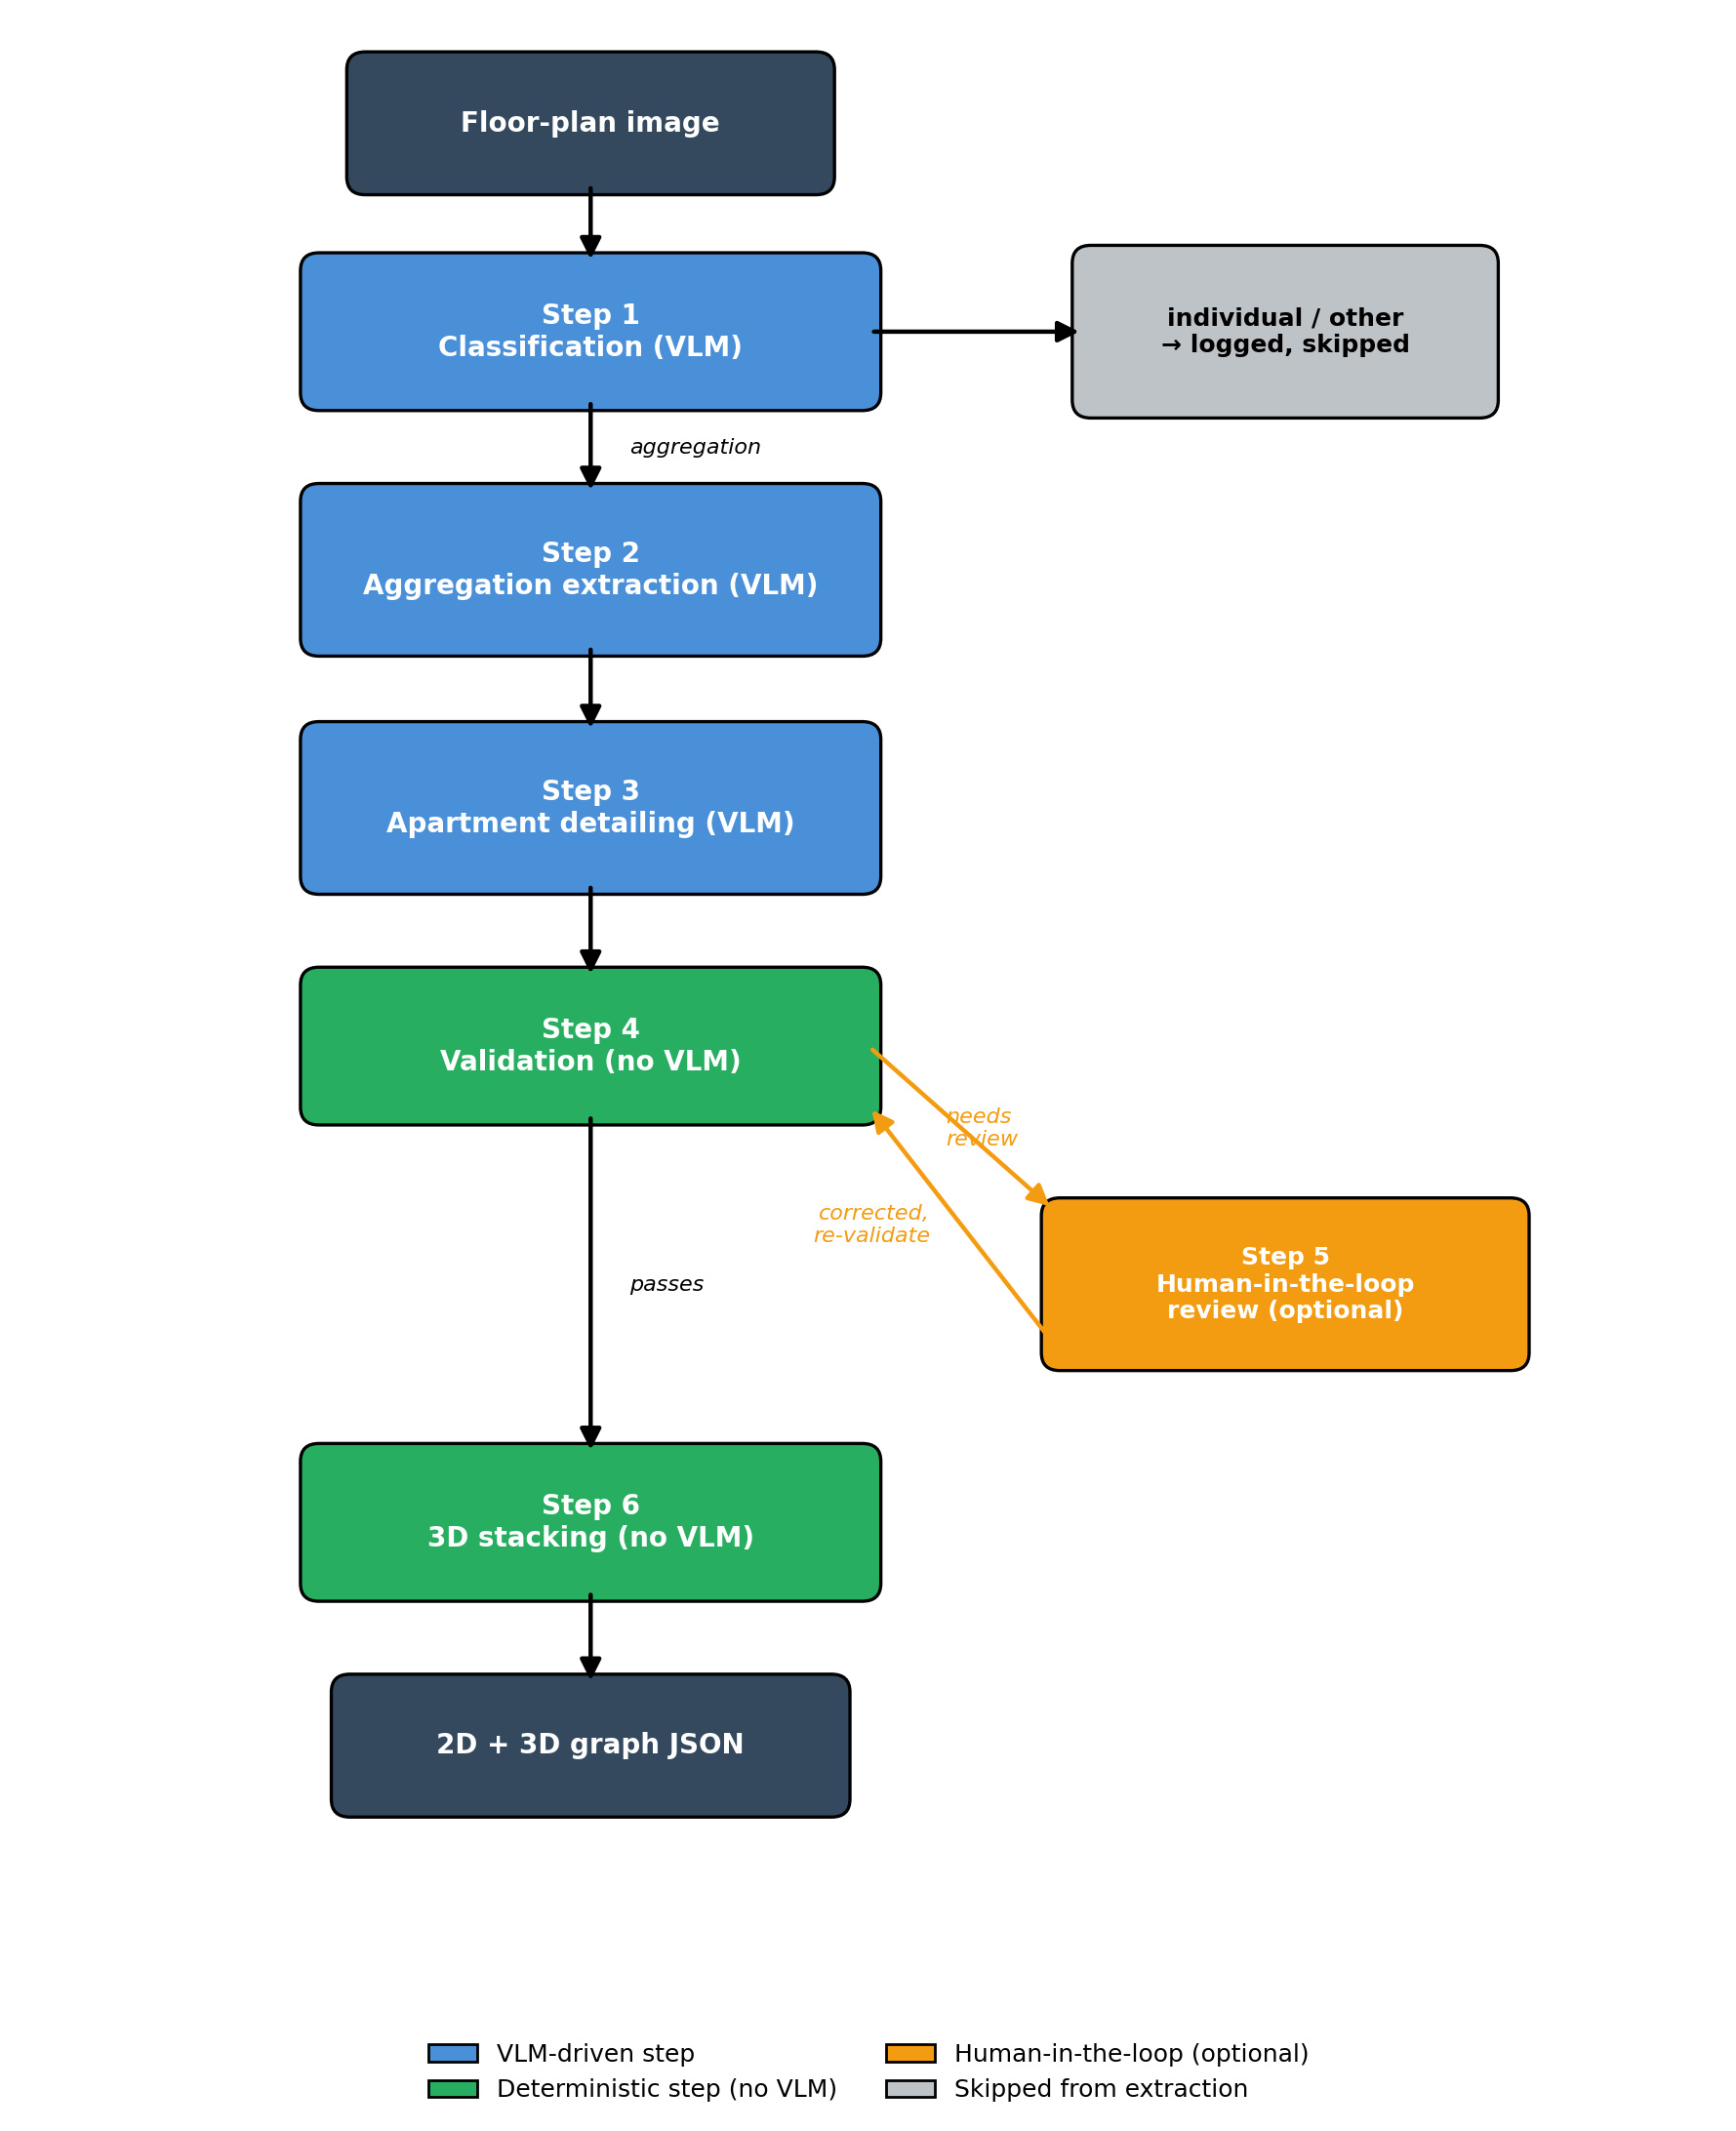
\includegraphics[width=1\linewidth]{figures/pipeline.png}
    \caption{Overview of the six-stage pipeline. A floor-plan image is first classified (Step~1); only \textit{aggregation} plans continue to the VLM-driven extraction (Steps~2--3), while \textit{individual} and \textit{other} plans are skipped. The assembled graph is checked by deterministic validation (Step~4): graphs that pass proceed directly to Step~6, whereas graphs that fail the connectivity checks take an optional detour to the interactive human-in-the-loop review (Step~5) and are then re-validated. Step~6 stacks the per-floor graphs into a 3D building. Steps~4 and~6 use no VLM.}
    \label{fig:pipeline}
\end{figure}

\begin{description}
    \item[Step 1 - Classification.] Each image is categorized as \textit{aggregation}, \textit{individual}, or \textit{other} utilizing a deterministic, three-class classification prompt. The \textit{other} class captures non-residential plans (e.g., offices, commercial locales, lobbies, parking, technical, or pure-circulation floors) that contain no dwellings to extract. Only \textit{aggregation} plans proceed to Steps~2 and 3; \textit{individual} and \textit{other} layouts are excluded from further extraction. To firmly anchor the model's visual taxonomy, canonical reference images are injected into the context window. The complete prompt formulation and the accompanying visual examples are detailed in Appendices~\ref{appendix:prompt-classify} and~\ref{appendix:ex-classify}, respectively.
    
    \item[Step 2 - Aggregation Analysis.] For multi-unit (\textit{aggregation}) plans, the VLM identifies discrete apartments, staircases, and elevator shafts as distinct graph nodes. It subsequently extracts the topological edges that connect these elements via shared circulation pathways. The full instructional prompt and its corresponding one-shot output example are provided in Appendices~\ref{appendix:prompt-aggregation} and~\ref{appendix:ex-aggregation}.
    
    \item[Step 3 - Apartment Detailing.] For each apartment node isolated in Step 2, the VLM is queried sequentially to extract internal room compositions and counts, fully detailing the localized sub-graph. The specialized prompt engineered to condition the model for this micro-scale extraction is documented in Appendix~\ref{appendix:prompt-details}.
    
    \item[Step 4 - Graph Assembly and Validation.] The extracted architectural features are merged into a unified 2D spatial graph, normalized, and subjected to a suite of deterministic structural validation checks. Enforcing the system's fault-tolerance taxonomy, graphs failing diagnostic topological checks are flagged and routed to the subsequent manual review phase, whereas outright strict parsing failures are isolated for error reporting.
    
    \item[Step 5 - Human-in-the-Loop Refinement.] An interactive feedback module allows an expert architect to provide corrective textual hints and reference image crops for flagged graphs. Rather than fine-tuning model weights, these corrections are persisted on disk as a dynamic visual memory, functioning as few-shot in-context learning examples for subsequent inference sessions. The review prompt and an illustrative in-context correction are included in Appendices~\ref{appendix:prompt-review} and~\ref{appendix:ex-review}.
    
    \item[Step 6 - 3D Alignment.] Single-floor 2D graphs belonging to the same building are spatially aligned along the Z-axis. This is achieved deterministically by linking vertical penetration nodes (e.g., staircases and elevators) across consecutive floors, yielding a cohesive, multi-story 3D topological graph.
\end{description}

% ============================================================
\chapter{Methodology}
\label{ch:methodology}

\section{Data Partitioning}
\label{sec:partitioning}

The combined corpus of \textit{1,276} floor plans is partitioned, at runtime, by \textbf{Step 1} into the three semantic categories established in Section~\ref{sec:problem} (\textit{aggregation}, \textit{individual}, \textit{other}). The classifier is a Qwen3-VL prompt running in deterministic mode---greedy decoding with $\text{do\_sample} = \mathrm{False}$---which makes the partition fully reproducible across executions.

Two reference images are supplied as one-shot in-context examples: \code{inca\_05.jpg} for the aggregation class and \code{inca\_50.jpg} for the individual class, selected for their textbook-clear visual cues (six labelled apartments around a central core with staircase and elevators, versus a single dwelling with fully labelled Catalan room names).

\section{Prompt Engineering Strategy}
\label{sec:prompts}

Because the VLM is never fine-tuned, the prompt is the only lever available to steer its behaviour. Four engineering techniques are applied consistently across all four VLM-driven steps of the pipeline.

\subsection{Persona Conditioning}

Every prompt opens with an architect persona, \eg:

\begin{quote}
\itshape
You are a professional architect specialised in residential building design and urban housing, with over fifteen years of experience reading and producing technical drawings for Catalan and Spanish social housing projects (IBAVI, IMPSOL, INCASOL).
\end{quote}

The persona biases the model towards the appropriate sub-distribution of its training data, treating domain-specific abbreviations (\textit{H}, \textit{EMC}, \textit{SC}, \textit{B}, \textit{Te}, \textit{P}) as familiar terminology rather than arbitrary tokens.

\subsection{Strong-Signal Enumeration}

Each prompt lists the unambiguous visual signals that characterise its target output. In the classification prompt, the aggregation class is described by signals such as repeated apartment identifiers (\textit{1A}, \textit{2B}, \textit{HA}), multiple kitchens, and shared courtyards; the individual class by signals such as exactly one kitchen, exactly one bathroom, and the absence of any apartment identifier. These enumerations give the model concrete features to verify pixel-locally before committing to a label.

\subsection{Decision Procedures}

For high-stakes decisions (classification, vertical-circulation detection), the prompt embeds an explicit ordered checklist that the model is instructed to follow. For example, the classification prompt encodes the following routine:

\begin{enumerate}
    \item Count the kitchens and bathrooms. If \emph{zero} of both are present (no habitable dwelling room at all---e.g.\ an office, parking, or pure-circulation floor), return \textit{other}. Shared stairs or corridors without any dwelling do not change this.
    \item Otherwise, count the kitchens. If exactly one, return \textit{individual}.
    \item Count the bathrooms. If exactly one, return \textit{individual}.
    \item Look for repeated apartment identifiers. If none, return \textit{individual}.
    \item Only if multiple kitchens, multiple self-contained units, and a shared circulation element are present, return \textit{aggregation}.
\end{enumerate}

This emulates the chain-of-thought paradigm without requiring the model to verbalise intermediate reasoning, which would inflate output length.

\subsection{Visual In-Context Examples}
\label{sec:visual-icl}

For tasks where visual judgement is decisive, the prompt is augmented with one or two reference images and their expected outputs. Step~1 receives two reference plans (one per class) with concise textual captions identifying their category. Step~2 receives a single canonical aggregation plan paired with its expected \textit{JSON} output, teaching the model both the visual pattern and the response schema simultaneously. Step~5 receives zero, one, two, or three image crops loaded from a persistent directory of human-confirmed examples (see Section~\ref{sec:human-review}).

To avoid circular reference, the wrapper skips an example whenever the target image is the example itself.

\section{2D Topological Extraction}

For each image, the partition assigned in Step~1 determines the next call. Only \textit{aggregation} plans enter the extraction path (Steps~2--3); \textit{individual} and \textit{other} plans are logged and skipped, as they carry no multi-unit graph to extract.

\subsection{Aggregation Analysis (Step 2)}

The VLM emits a list of \emph{nodes} (apartments, staircases, elevators) and \emph{edges} (door- or landing-mediated connections). Apartments are anchored by their principal-entrance \emph{door\_position}, expressed as a percentage of image dimensions; staircases and elevators carry a centroid \emph{position}. The one-shot reference described in Section~\ref{sec:visual-icl} is provided to enforce both visual pattern and schema adherence.


\subsection{Apartment Detailing (Step 3)}

The output of Step~2 yields, for each aggregation plan, a list of apartments to inspect individually. The VLM is re-invoked with a localised prompt (Appendix \ref{appendix:prompt-details}) of the form \textit{``focus only on the apartment labelled X, located approximately at $[x, y]$\,\ldots''} and produces a \textit{JSON} object encoding the room inventory: $n_{\text{bedrooms}}$, $n_{\text{bathrooms}}$, $n_{\text{kitchens}}$, $n_{\text{living rooms}}$, $n_{\text{terraces}}$, $\text{has\_corridor}$, $\text{total\_rooms}$, and the list of visible room labels. Individual plans are skipped.

\section{Graph Assembly and Validation}
\label{sec:assembly}

In Step 4, the structured outputs from the preceding extraction phases are algorithmically merged into a unified 2D spatial graph $G = (V, E)$. Within this graph, apartment nodes encapsulate their internal room inventories (extracted in Step 3) as a nested \texttt{details} attribute. 

To ensure architectural feasibility, the assembled graph is subjected to six deterministic validation checks. These are categorized into \emph{strict constraints} (whose failure marks the graph as topologically invalid) and \emph{diagnostic indicators} (which lower a quality score and flag the graph for human review, but do not inherently invalidate the data structure).

\begin{description}
    \item[Minimum Apartment Threshold (Strict).] At least two apartment nodes must be present; otherwise, the plan does not constitute a genuine multi-unit aggregation.
    \item[Global Connectivity (Strict).] All nodes must belong to a single connected component, ensuring the floor plan represents a contiguous building layout.
    \item[Local Node Connectivity (Strict).] Every apartment node must possess at least one edge.
    \item[Vertical Circulation Presence (Diagnostic).] At least one staircase or elevator node must be identified within the graph.
    \item[Circulation Reachability (Diagnostic).] Each apartment must be able to reach a vertical-circulation node via the graph's edges.
    \item[Spatial Uniqueness (Diagnostic).] No two nodes may occupy the exact same $[x, y]$ topological coordinate.
\end{description}

While related, these checks serve distinct purposes. Strict connectivity merely ensures an apartment is not isolated. Conversely, the reachability check catches hallucinated, illegal edges drawn directly between apartments. Reachability remains a diagnostic indicator because an untraced corridor is usually a minor extraction oversight, not a catastrophic structural failure.

Following validation, each graph is appended with automated metadata: a \texttt{passed} boolean (indicating all strict constraints were met) and a \texttt{score} (the fraction of the six checks successfully passed). In accordance with the \emph{Diagnostic Preservation} principle outlined in Section~\ref{sec:principles}, failed checks are permanently embedded as \texttt{flags} inside the \textit{JSON} structure rather than triggering data deletion. A complete example of the resulting 2D graph object, with all node, edge, and metadata fields, is provided in Appendix~\ref{appendix:json-2d}.

This metadata dictates the routing logic for the pipeline. Graphs that pass the strict constraints but fail the diagnostic indicators (e.g., missing or unreachable vertical circulation) trigger a \texttt{needs\_human\_review} flag and are directly routed to the Human-in-the-Loop interface (Step 5). Conversely, graphs that fail strict structural constraints are retained purely for quantitative error logging and are excluded from the human review cycle.

\section{Human-in-the-Loop Refinement}
\label{sec:human-review}

Even with careful prompting, the model occasionally fails to detect elements that an architect would identify immediately, particularly stair cores and elevator shafts drawn in unusual styles. Step~5 provides an interactive command-line tool that lets the architect inject two forms of feedback.

\paragraph{Textual hint.} A free-text description of the missed element (\eg, \textit{``a staircase is present in the central core but was not detected''}) is interpolated into a re-extraction prompt that asks the model to re-examine the image with this knowledge.

\paragraph{Reference image crop.} The architect may additionally supply a cropped image of the missed element (\eg, the staircase symbol used throughout the dataset). The crop is copied to a persistent directory \code{outputs/human\_review\_examples/} organised by element type (staircase or elevator). On every subsequent VLM invocation, up to three crops per type are re-loaded and prepended as few-shot visual references. This persists the correction across sessions without any model fine-tuning.

This design treats human feedback as a form of long-term visual memory: once an architect has annotated one staircase, the model is far more likely to recognise similar staircases across the rest of the dataset.

\section{3D Spatial Alignment}
\label{sec:3d}

A building is not a stack of independent floors but a connected three-dimensional structure: the staircase that lands on floor $k$ must rise to floor $k+1$, and likewise for elevators. Step~6 makes this explicit.

Let $\mathcal{B} = \{G_0, G_1, \ldots, G_{F-1}\}$ be the set of per-floor aggregation graphs belonging to the same building, ordered by floor index. The 3D graph $G_{3D} = (V_{3D}, E_{3D})$ is constructed in three phases.

\paragraph{Phase 1 - Node globalisation.} Each node $v \in V_{f}$ on floor $f$ is assigned a global identifier
\[
    \mathrm{id}_{3D}(v) = f \times 10^{6} + \mathrm{id}_{2D}(v),
\]
chosen so that the floor index can be recovered by integer division and the intra-floor identifier by modulo.

\paragraph{Phase 2 - Horizontal-edge replication.} For each floor $f$ and each edge $(u, v) \in E_{f}$, an edge of type \emph{horizontal} is added to $E_{3D}$, tagged with the floor index. These edges encode the within-floor accessibility relationships extracted in Step~2.

\paragraph{Phase 3 - Vertical alignment.} For every pair of consecutive floors $(f, f+1)$, vertical-circulation nodes are paired by spatial proximity. Let $S_{f}$ and $S_{f+1}$ denote the staircase node sets on floors $f$ and $f+1$; a greedy nearest-neighbour matching is performed on their position vectors:
\[
    \mathrm{match}(s_i, s_j^{\star}) \quad \text{such that} \quad
    s_j^{\star} = \argmin_{s_j \in S_{f+1} \setminus \mathrm{used}} \lVert \mathbf{p}(s_i) - \mathbf{p}(s_j) \rVert_{2}.
\]
The same procedure is applied independently to the elevator node sets $L_{f}$ and $L_{f+1}$. Each matched pair contributes one \emph{vertical} edge tagged with the type of the circulation element. Unmatched extras---\eg, a service staircase that exists on only some floors ---are left disconnected and generate an \code{asymmetric\_circulation} flag.

\paragraph{Post-conditions.} The resulting graph is finally checked for global connectivity and for the presence of at least one vertical edge per floor pair. Buildings violating these conditions are flagged but retained. Figure~\ref{fig:3d-example} shows an example of the resulting 3D graph, and its full JSON schema is given in Appendix~\ref{appendix:json-3d}.


While the production pipeline replicates a single floor, the same alignment routine also accepts a sequence of distinct per-floor graphs, enabling true multi-floor assembly when separate floor plans of the same building are available.

\begin{figure}[ht]
    \centering
    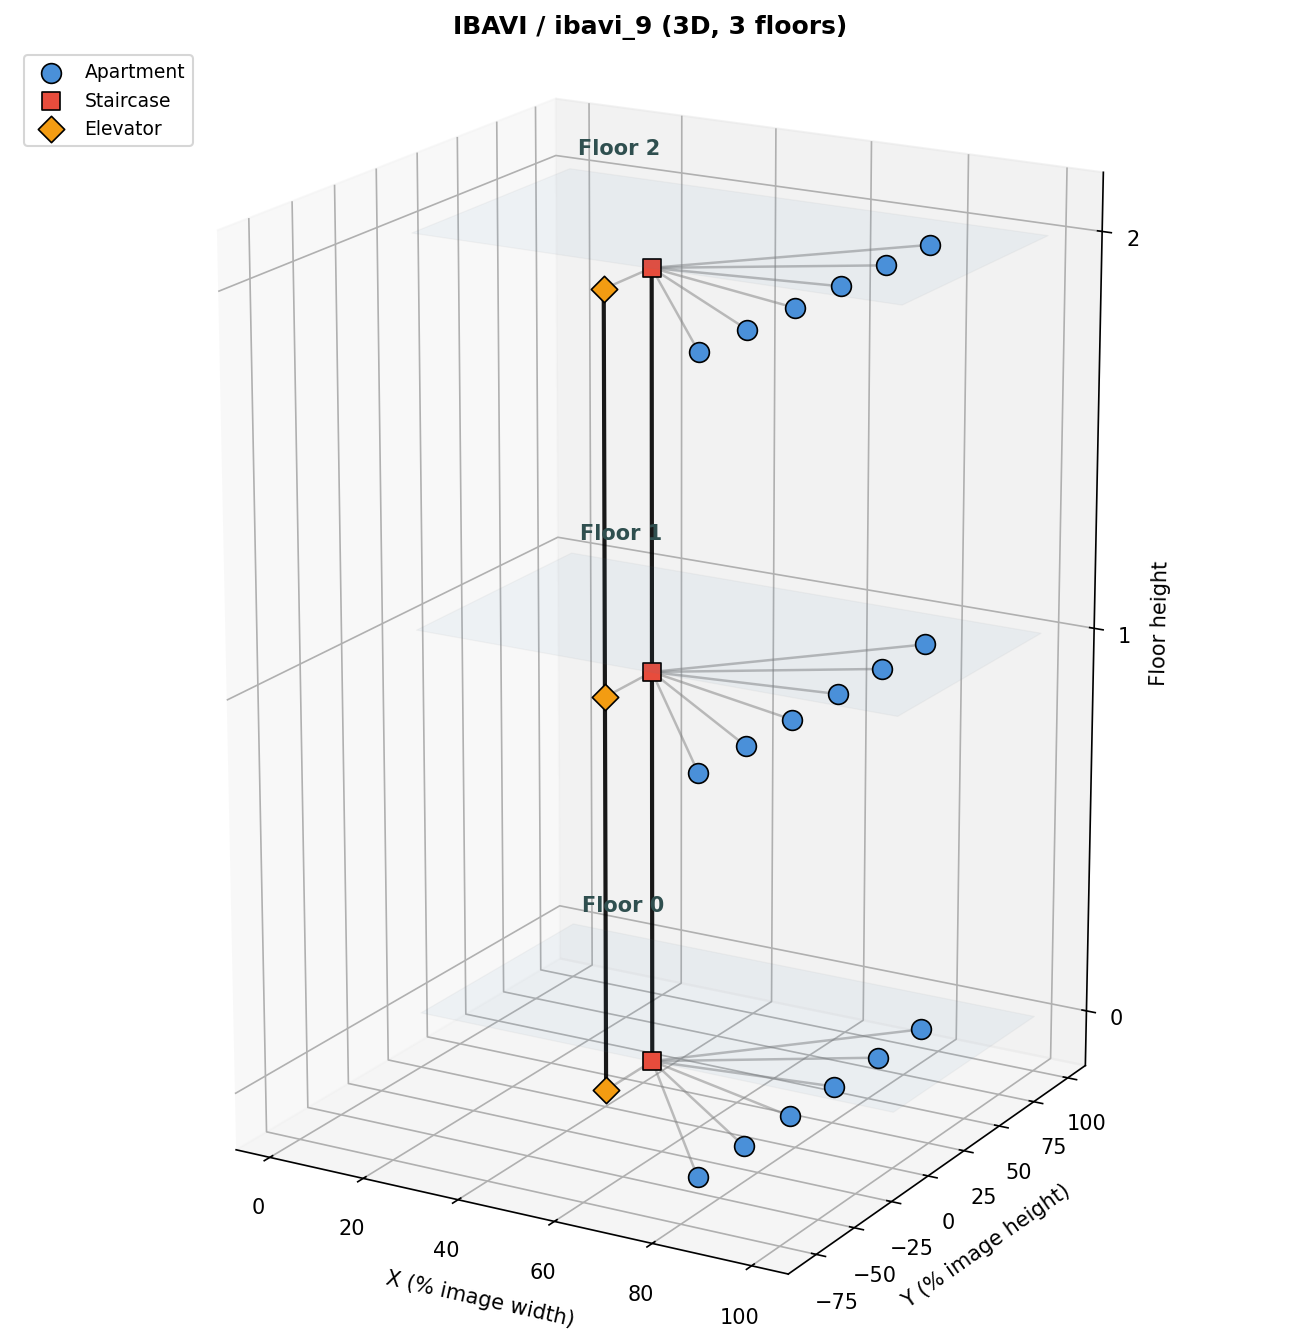
\includegraphics[width=0.7\textwidth]{figures/ibavi_9_3d.png}
    \caption{Example 3D building graph produced by Step~6. A single floor is
    replicated across three storeys (Floor~0--2); the shared staircase (red) and elevator (orange) of each floor are linked vertically by nearest-position matching, forming the building's vertical circulation core, while each floor's apartments (blue) remain connected only within their own level.}
    \label{fig:3d-example}
\end{figure}


\section{Validation Strategy}
\label{sec:validation}

The absence of ground truth precludes conventional supervised metrics computed over the whole corpus. Validation in this thesis therefore relies on two complementary criteria, applied jointly to provide convergent evidence of correctness.

\paragraph{Deterministic structural checks.} Every extracted graph is subjected to the six structural checks of Section~\ref{sec:assembly} (apartment count, connectivity, isolation, connector presence, connector reachability, and duplicate positions). These require no ground truth and yield a per-graph pass rate and quality score over the full dataset.

\paragraph{Manual classification ground truth.} For Step~1 specifically, the entire corpus of 1,276 plans was manually labelled by the author, assigning each image its true class (\textit{aggregation}, \textit{individual}, or \textit{other}). This exhaustive labelling enables exact classification metrics---accuracy, per-class precision, recall, and $F_1$, and a full confusion matrix---against the model's predictions, rather than a sampled estimate.

\paragraph{Manual spot-checks of extraction.} For the extraction steps (Steps~2--3), where exhaustive labelling of every node and edge is infeasible, a random sample of approximately 30 plans is reviewed by the author, who compares each extracted graph against the original image and records missing nodes, spurious nodes, incorrect connections, and incorrect room types. This yields an approximate accuracy estimate that, while not a substitute for full ground truth, provides a credible lower bound on extraction reliability.



% ============================================================
\chapter{Implementation}
\label{ch:implementation}

This chapter documents the engineering decisions that translate the methodology of Chapter~\ref{ch:methodology} into a reproducible software artefact.

\section{Model Selection}
\label{sec:model_selection}

Three critical constraints governed the selection of the Vision-Language Model (VLM): (i) \emph{open weights}, ensuring scientific reproducibility and eliminating the financial and latency overhead of commercial cloud APIs across thousands of inference steps; (ii) \emph{native multi-image support}, an absolute prerequisite for few-shot visual in-context learning; and (iii) \emph{deployability within a 16\,GB VRAM footprint}, matching the capacity of the remote NVIDIA RTX A5000 server available for full-dataset processing.

Within these rigid constraints, the Qwen3-VL family was prioritized over alternatives such as LLaVA, InternVL, and BLIP-2 for two primary reasons. First, Qwen3-VL demonstrates state-of-the-art performance on document-understanding benchmarks (e.g., DocVQA, ChartQA). This capability is paramount given the high density of textual abbreviations and dimensional annotations embedded within social-housing blueprints. Second, it natively processes interleaved multi-image inputs, whereas several competing architectures require the delicate and computationally inefficient concatenation of multiple images into a single visual canvas.

To facilitate both iterative development and large-scale extraction, two specific variants of the model were utilized:

\begin{description}
    \item[Qwen3-VL-4B-Instruct] ($\approx$ 8\,GB in \texttt{bfloat16}) --- utilized for local development, prompt engineering, and rapid prototyping on an NVIDIA RTX 2070 8\,GB GPU, enabling efficient code iteration prior to server deployment.
    \item[Qwen3-VL-8B-Instruct] ($\approx$ 16\,GB in \texttt{bfloat16}) --- deployed for the final production inference on the remote NVIDIA RTX A5000. Its expanded parameter capacity yields significantly higher reliability when extracting edge cases, such as plans with rotated text labels or partially occluded architectural elements.
\end{description}

A larger Mixture-of-Experts (MoE) variant, Qwen3-VL-30B-A3B-Instruct-FP8, was evaluated but ultimately rejected. Although its 3B active-parameter inference footprint appears theoretically viable, the entire 30B parameter set must still reside in VRAM. Furthermore, FP8 precision compute is strictly restricted to Hopper and Ada Lovelace microarchitectures. The A5000 supports neither of these requirements, rendering the 30B MoE model untenable for this hardware environment.

\section{Inference Infrastructure}

The model is loaded through Hugging Face Transformers ($\geq$ 4.46) using the auto-class \code{AutoModelForImageTextToText} (the explicit \code{Qwen2\_5\_VLForConditionalGeneration} class produces a weight-shape mismatch on Qwen3-VL checkpoints and must be avoided). The \code{dtype} parameter is set to \code{torch.bfloat16}, balancing numerical accuracy and memory footprint.

A single \code{VLMClient} wrapper handles model loading (once per process) and exposes a single \code{query()} method. The method accepts an optional list of \code{example\_images} (each a path-and-caption tuple) that are prepended to the prompt, and a \code{deterministic} boolean that switches between greedy and sampling decoding. This single abstraction is used uniformly across all six pipeline steps, isolating generation parameters from prompt content.

\section{Hardware and Deployment}
\label{sec:hardware_and_deploy}

As introduced in Section~\ref{sec:model_selection}, the inference pipeline was deployed across two distinct hardware environments to balance agile prototyping with large-scale processing capabilities:

\paragraph{Local Environment.} A workstation running Windows 11, equipped with an NVIDIA RTX 2070 GPU (8\,GB VRAM), is utilized to host the smaller 4B-parameter model variant. Rather than executing the full-scale extraction pipeline, this constrained environment serves strictly as an experimental sandbox. It is dedicated to rapid prompt engineering on micro-batches (typically five to ten floor plans) and facilitates the inherently interactive Human-in-the-Loop (HITL) visual refinement phase.

\paragraph{Remote Environment.} An Ubuntu server equipped with an NVIDIA A5000 (24GB VRAM) hosts the 8B model and runs the pipeline against the full 1,276-image corpus. Access is mediated by SSH and the Visual Studio Code Remote-SSH extension, which allows the same source tree to be edited locally and executed remotely without manual file transfers. The full-corpus extraction is launched as a single long-running command over this SSH session; because the pipeline writes each graph to disk immediately after extraction, partial progress is preserved even if the session is interrupted.

\section{Software Architecture}

The codebase, publicly available as an open-source repository (Appendix~\ref{appendix:code}), is organised around the six pipeline steps, with a thin orchestration layer and a small number of cross-cutting utilities.

\begin{itemize}
    \item \code{src/config.py} --- centralised configuration: paths, model identifiers, hyperparameters, and the canonical one-shot example images.
    \item \code{src/vlm\_client.py} --- the \code{VLMClient} wrapper.
    \item \code{src/step1\_classify.py} through \code{src/step6\_stack3d.py} --- one module per pipeline step, each exposing both a single-image function and a batch function.
    \item \code{src/pipeline.py} --- command-line orchestrator that composes the six steps and writes outputs to disk.
    \item \code{src/utils/json\_parser.py} --- robust \textit{JSON} extractor that tolerates the additional prose VLMs sometimes emit before or after the JSON block.
    \item \code{src/utils/visualization.py} --- NetworkX-based graph rendering for visual quality assurance.
    \item \code{prompts/*.txt} --- prompt templates kept outside the code so that they can be edited without re-deploying the pipeline.
\end{itemize}

Outputs are written to a stable directory layout (\code{outputs/graphs}, \code{outputs/visualizations}, \code{outputs/logs}, \code{outputs/stats}, \code{outputs/human\_review\_examples}), enabling incremental processing: re-runs only regenerate missing artefacts.

\section{Reproducibility}
\label{sec:reproducibility}

To ensure the strict scientific reproducibility of the proposed pipeline, three operational measures are enforced. First, probabilistic variance is explicitly suppressed during rigid tasks (such as the initial layout classification) by enforcing deterministic decoding configurations (e.g., zero temperature). Second, all canonical reference images and preserved Human-in-the-Loop (HITL) visual crops are version-controlled alongside the source code. This guarantees that any future execution of the pipeline is conditioned on the exact same in-context visual memory. Third, the computational environment is rigorously standardized: software dependencies are strictly pinned within a \texttt{requirements.txt} file, and the Vision-Language Model checkpoint is instantiated using an exact cryptographic revision hash, rather than relying on a floating repository pointer (e.g., the \texttt{main} branch of the Hugging Face Hub). The full source code, prompts, and evaluation scripts are publicly available as an open-source repository (Appendix~\ref{appendix:code}).

Consequently, the entire extraction pipeline can be reproduced end-to-end via a single modular command:

\begin{lstlisting}[language=bash]
python -m src.pipeline --dataset INCASOL
\end{lstlisting}

\noindent This command automatically processes the specified dataset corpus, sequentially executing image classification, topological graph extraction, and deterministic structural validation, before archiving the finalized \textit{JSON} artifacts to the \texttt{outputs/} directory.


% ============================================================
\chapter{Experiments \& Results}
\label{ch:experiments}

\section{Experimental Setup}
\label{sec:exp-setup}

The methodology is evaluated on three real-world datasets from the target domain of Catalan social-housing architecture. The plans were provided by the project co-director from internal institutional archives:

\begin{itemize}
    \item \textbf{IBAVI} --- plans from the \textit{Institut Balear de
    l'Habitatge} (36 plans).
    \item \textbf{IMPSOL} --- plans from the \textit{Institut Metropolità de
    Promoció de Sòl i Gestió Patrimonial} (348 plans), spanning both
    clearly-drafted CAD plans and harder cases such as hand-drawn drawings.
    \item \textbf{INCASOL} --- plans from the \textit{Institut Català del Sòl}
    (892 plans), the largest of the three sources.
\end{itemize}

All three datasets contain instances of the three classes introduced
previously (\textit{aggregation}, \textit{individual}, and \textit{other}). Table~\ref{tab:dataset-dist} reports the ground-truth class distribution per source, established by manual labelling (described below).

\begin{table}[ht]
\centering
\begin{tabular}{@{}lrrrr@{}}
\toprule
\textbf{Source} & \textbf{Aggregation} & \textbf{Individual} & \textbf{Other} & \textbf{Total} \\
\midrule
IBAVI   &   9 &  27 & 0 &   36 \\
IMPSOL  & 168 & 180 & 0 &  348 \\
INCASOL & 488 & 403 & 1 &  892 \\
\midrule
\textbf{Total} & \textbf{665} & \textbf{610} & \textbf{1} & \textbf{1{,}276} \\
\bottomrule
\end{tabular}
\caption{Ground-truth class distribution per dataset source, from exhaustive
manual labelling of all 1{,}276 plans. Aggregation plans are the extraction
targets; individual and other plans carry no multi-unit graph.}
\label{tab:dataset-dist}
\end{table}

\paragraph{Evaluation scope.} We evaluate the three VLM-driven extraction stages that determine output quality --- classification (Step~1), aggregation analysis (Step~2), and apartment detailing (Step~3) --- following the validation strategy of Section~\ref{sec:validation}.

\paragraph{Ground-truth construction.} Two evaluation references were built by the author. For \textbf{Step~1}, all 1{,}276 plans were manually labelled with their true class, applying the rule that a plan is \textit{aggregation} only if it contains two or more self-contained dwellings sharing a vertical-circulation core; side-by-side unit typologies (e.g., ``Tipus A / Tipus B'' catalogues) are
\textit{individual}, and non-dwelling drawings are \textit{other}. This exhaustive labelling permits exact classification metrics rather than a sampled estimate. For \textbf{Steps~2--3}, where node- and edge-level labelling of every graph is infeasible, a random spot-check of approximately 30 aggregation plans was reviewed against the source images.

\paragraph{Metrics.} Step~1 is reported with a full classification report (accuracy, per-class precision, recall, and $F_1$) and a confusion matrix. 
Steps~2--3 are assessed through the six deterministic structural checks of Section~\ref{sec:assembly} (yielding a per-graph pass rate and mean quality score) and the spot-check error categories: missing nodes, spurious nodes, incorrect connections, and incorrect room types.

\paragraph{Outcome taxonomy.} Each plan routed into extraction ends in exactly one of three states, used consistently throughout this chapter:
\begin{description}
    \item[Passing.] A graph was produced and satisfied all hard structural checks.
    \item[Flagged (soft).] A graph was produced but failed a soft check (missing
    or unreachable vertical circulation) and is routed to human review.
    \item[Extraction failure.] The model produced no parseable graph; no JSON exists, and the case is logged separately.
\end{description}

\noindent The model and hardware experimental settings are detailed in
Sections~\ref{sec:model_selection} and~\ref{sec:hardware_and_deploy}; briefly, the \mbox{Qwen3-VL-8B-Instruct} model (roughly 16GB in \code{bfloat16}) is used, running on an NVIDIA RTX A5000 GPU with 24GB of VRAM.


\section{Classification Performance (Step 1)}
\label{sec:exp-classification}

Because the entire dataset was manually annotated, the classifier's performance can be evaluated exhaustively rather than through statistical sampling. Across the complete corpus of 1,276 floor plans, Step~1 achieves a robust overall accuracy of \textbf{90.05\%} (1,149 correct classifications). Table~\ref{tab:class-report} details the per-class precision, recall, and $F_1$ scores, while Table~\ref{tab:confusion} presents the comprehensive confusion matrix.

\begin{table}[ht]
\centering
\begin{tabular}{@{}lrrrr@{}}
\toprule
\textbf{Class} & \textbf{Precision} & \textbf{Recall} & \textbf{$F_1$} & \textbf{Support} \\
\midrule
Aggregation & 0.889 & 0.938 & 0.913 & 665 \\
Individual  & 0.926 & 0.861 & 0.892 & 610 \\
Other       & 0.000 & 0.000 & 0.000 &   1 \\
\midrule
\textbf{Accuracy}     & \multicolumn{4}{r}{0.901 \quad (1{,}149 / 1{,}276)} \\
\textbf{Macro avg}    & 0.605 & 0.600 & 0.602 & 1{,}276 \\
\textbf{Weighted avg} & 0.906 & 0.901 & 0.902 & 1{,}276 \\
\bottomrule
\end{tabular}
\caption{Step~1 classification report against the manually labelled ground truth. Because the \textit{other} class contains only a single ground-truth instance, its per-class scores lack statistical significance.}
\label{tab:class-report}
\end{table}

\begin{table}[ht]
\centering
\begin{tabular}{@{}lrrr@{}}
\toprule
 & \multicolumn{3}{c}{\textbf{Predicted}} \\
\cmidrule(l){2-4}
\textbf{True} & Aggregation & Individual & Other \\
\midrule
Aggregation & \textbf{624} & 41 & 0 \\
Individual  & 78 & \textbf{525} & 7 \\
Other       & 0 & 1 & \textbf{0} \\
\bottomrule
\end{tabular}
\caption{Confusion matrix for the Step~1 layout classification (rows: ground-truth class; columns: predicted class). Diagonal entries represent correct predictions.}
\label{tab:confusion}
\end{table}

\paragraph{Performance on Principal Classes.} The classifier demonstrates highly effective predictive capabilities on the two primary classes of interest. The \textit{aggregation} class achieves an $F_1$ score of 0.913 and a high recall of 0.938. This high recall is crucial: the model successfully isolates the vast majority of true multi-unit building floors, which is the pipeline's operational priority since only aggregation plans proceed to topological extraction. The \textit{individual} class similarly performs well, yielding an $F_1$ score of 0.892. The weighted-average $F_1$ score of 0.902 further underscores this balanced, high-fidelity classification across the bulk of the corpus.

\paragraph{The Dominant Error: Typology Catalogues.} The confusion matrix reveals that the most frequent misclassification is the \emph{78 individual plans predicted as aggregation}---constituting by far the largest off-diagonal value. Manual qualitative inspection confirms that these cases are predominantly \emph{typology catalogues}: archival sheets displaying several distinct architectural unit types side-by-side (e.g., ``Tipus A'', ``Tipus B'') alongside their respective area tables. Because these sheets visually present multiple kitchens, bathrooms, and discrete unit boundaries, the vision-language model logically, though incorrectly, interprets them as true multi-unit floor layouts. This represents the pipeline's most disruptive error mode, as it routes non-building plans into the topological extraction phase, ultimately yielding empty or degenerate graphs (discussed further in Section~\ref{sec:exp-failure}). Conversely, the opposite error (41 aggregations misclassified as individual) occurs less frequently and is typically caused by faint, low-contrast, or label-sparse historical scans where the shared central circulation core is visually illegible.

\paragraph{Statistical Insignificance of the \textit{Other} Class.} Only a single plan in the entire 1,276-image corpus is genuinely non-residential (\textit{other}). While the model predicted the \textit{other} class seven times, none matched this solitary ground-truth instance. Consequently, the per-class scores for \textit{other} evaluate to zero and lack statistical significance---artificially depressing the macro-average $F_1$ (0.602) without impacting the weighted average. In practice, the conceptual three-class taxonomy collapses into a near-binary classification problem for this specific dataset. Genuine non-dwelling plans are virtually absent from these Catalan social-housing archives, meaning the \textit{other} category is too sparsely represented to be reliably assessed, though it remains structurally necessary for the pipeline's generalizability.

\paragraph{Verification of Determinism.} In strict adherence to the reproducibility principles outlined in Section~\ref{sec:reproducibility}, Step~1 utilizes greedy decoding mechanisms. Consequently, these classification metrics are fully deterministic; re-executing the classifier yields identical categorical labels across the entire corpus without probabilistic variance.


\section{2D Extraction Quality (Steps 2--3)}
\label{sec:exp-extraction}

This section evaluates the structural quality of the 2D graphs produced for the plans classified as \textit{aggregation}. Of the 702 plans routed into extraction, 11 produced no parseable graph (hard extraction failures, analysed in Section~\ref{sec:exp-failure}); the remaining 691 graphs were assembled and subjected to the six deterministic checks of Section~\ref{sec:assembly}.

\subsection{Structural Validation Results}

Across the 691 extracted graphs, \textbf{623 (90.2\,\%) pass all hard structural checks}, with a mean quality score of \textbf{0.924} (the fraction of the six checks satisfied, averaged over all graphs). The 68 graphs that do not pass fail at least one hard check; a subset is additionally routed to human review. Table~\ref{tab:val-rules} reports how often each individual check fails.

\begin{table}[ht]
\centering
\begin{tabular}{@{}llr@{}}
\toprule
\textbf{Check} & \textbf{Type} & \textbf{Failures} \\
\midrule
\code{no\_dup\_positions}            & soft & 162 \\
\code{all\_connected}                & hard & 65 \\
\code{has\_apartments}               & hard & 28 \\
\code{has\_connectors}               & soft & 28 \\
\code{every\_apt\_reaches\_connector} & soft & 28 \\
\code{no\_isolated\_apt}             & hard & 3 \\
\bottomrule
\end{tabular}
\caption{Per-check failure counts over the 691 extracted graphs. A graph may fail several checks at once, so the counts are not mutually exclusive. Only the hard checks determine the \emph{passing} verdict; the soft checks lower the quality score and may route a graph to human review.}
\label{tab:val-rules}
\end{table}

\subsection{Analysis of the Failure Counts}

\paragraph{Duplicate positions are the most frequent but least severe issue.}
The most common flag, \code{no\_dup\_positions} (162 graphs), is a \emph{soft} check: it fires whenever two nodes are assigned the same $[x, y]$ percentage coordinate. This reflects coordinate imprecision in the model's spatial estimates---two apartments placed at the same point---rather than a topological error, and does not by itself invalidate a graph.

\paragraph{Connectivity failures are the main driver of non-passing graphs.}
The \code{all\_connected} check fails on 65 graphs---the dominant \emph{hard} failure. These are graphs that split into more than one connected component, typically because an apartment (or a connector) was extracted but its edge to the shared circulation was not traced. This is the failure mode the no-fabrication edge rule (Section~\ref{sec:assembly}) deliberately tolerates: the model is
instructed to omit an edge it cannot see rather than invent one, so genuinely untraceable connections surface here as disconnections rather than as hallucinated edges.

\paragraph{Empty graphs reflect upstream misclassification.} The 28 graphs that fail \code{has\_apartments} (fewer than two apartment nodes) coincide with the 28 that fail \code{has\_connectors} and \code{every\_apt\_reaches\_connector}:
these are near-empty graphs produced from plans that are not genuine
aggregations. Manual inspection confirms they are predominantly the typology catalogues misclassified in Step~1 (Section~\ref{sec:exp-classification}); the extraction model correctly declines to fabricate apartments, emitting an empty or near-empty graph instead. The failure therefore originates in classification, not extraction---a point developed in Section~\ref{sec:exp-failure}.

\paragraph{Summary.} Excluding the empty graphs caused by upstream
misclassification, the extraction stage produces structurally valid 2D graphs for the large majority of true aggregation plans, and its errors are dominated by missing edges (conservative under-connection) rather than fabricated structure.

\subsection{Manual Spot-Check of Extraction}
\label{sec:exp-spotcheck}

The structural checks of Section~\ref{sec:exp-extraction} verify topological plausibility but cannot confirm \emph{semantic} correctness---a graph may be well-formed yet miscount apartments, hallucinate a connector, or assign the wrong room inventory. To assess this, a stratified random sample of 30 plans whose graphs passed the structural checks was reviewed against the source images, recording, per graph, the number of missing nodes, spurious nodes,
incorrect edges, and apartments with an incorrect room inventory.

Of the 30 sampled plans, 7 are revealed by the review to be \emph{not} genuine aggregations: they were misclassified in Step~1 (predominantly typology catalogues, Section~\ref{sec:exp-classification}) yet still produced a structurally valid graph, and are therefore semantic failures by construction. The remaining 23 plans are true aggregations and form the basis of the extraction-quality figures below.

\paragraph{Overall correctness.} Among the 23 true-aggregation graphs, only 3 (13\,\%) were judged \emph{fully correct}---a faithful node-for-node and edge-for-edge match to the plan. The remaining 20 contained at least one semantic error invisible to the structural checks. Table~\ref{tab:spotcheck} breaks these errors down by category.

\begin{table}[ht]
\centering
\begin{tabular}{@{}lrr@{}}
\toprule
\textbf{Error category} & \textbf{Graphs affected} & \textbf{Total instances} \\
\midrule
Missing nodes (apartments / connectors) & 10 (43\,\%) & 18 \\
Spurious nodes                          & 15 (65\,\%) & 24 \\
Incorrect edges                         & 2 (9\,\%)   & 12 \\
Incorrect room inventory                & 5 (22\,\%)  & 15 \\
\bottomrule
\end{tabular}
\caption{Semantic error rates over the 23 true-aggregation graphs in the spot-check sample. ``Graphs affected'' counts graphs with at least one error of that category; ``total instances'' sums the errors across all graphs. A graph may exhibit several categories, so the rows are not mutually exclusive.}
\label{tab:spotcheck}
\end{table}

\paragraph{Node counting is the dominant error.} The review confirms that the model's principal weakness is \emph{counting apartments}, not connecting them: spurious nodes affect 65\,\% of graphs and missing nodes 43\,\%, whereas incorrect edges are rare (9\,\%). The error is bidirectional---the model both over-counts (\eg, splitting a service space or a public zone into extra apartments) and under-counts (\eg, merging or omitting units on dense, radial, or row layouts). In several cases the model's own \code{building\_analysis} field states a different apartment count from the one it ultimately emits, exposing an internal inconsistency. The scarcity of edge errors is a direct consequence of the no-fabrication rule (Appendix~\ref{appendix:prompt-aggregation}): once nodes are placed, the hub-and-spoke wiring to the core is usually correct.

\paragraph{Room inventory and connectors.} Incorrect room inventories appear in 22\,\% of graphs, typically a bedroom count that contradicts the plan's typology legend (\eg, a ``3D'' three-bedroom type extracted with two bedrooms). Connector errors---a missing elevator, or an elevator hallucinated where the plan shows only a stair or a central distributor---account for part of the node errors above and recur on plans whose vertical circulation is drawn ambiguously.

\paragraph{Interpretation.} The 13\,\% fully-correct rate should be read against the strictness of the criterion: a single miscounted apartment marks an entire graph as not fully correct, even when the connectivity and the majority of nodes are right. The structural pass rate of Section~\ref{sec:exp-extraction} (90.2\,\%) and this semantic rate are therefore complementary: the pipeline reliably produces \emph{well-formed} graphs, but exact node-level fidelity on dense or legend-driven plans remains the principal open challenge, and is the main target of the human-in-the-loop refinement evaluated next.


\section{Human-in-the-Loop Refinement (Step 5)}
\label{sec:exp-hitl}

This section evaluates the human-in-the-loop review that follows Step~4. The validation stage flagged 28 graphs as needing review (missing or unreachable vertical circulation). However, as established in Sections~\ref{sec:exp-classification} and~\ref{sec:exp-spotcheck}, the large majority of these flags are not extraction errors but \emph{upstream misclassifications}: typology catalogues and single dwellings wrongly routed into extraction, which the model had correctly emptied. Of the 28 flagged graphs, only \textit{inca\_555.jpg} was a correct aggregation whose graph warranted correction; the remainder were skipped during the interactive session as they carry no real building structure to refine.

For \textit{inca\_555.jpg}, the initial extraction (Figure~\ref{fig:inca_555}) over-counted the dwellings---emitting eight apartments and two redundant circulation cores (two staircases and two elevators) instead of the five apartments and single core actually present---and left one apartment node disconnected from any connector. The model had been misled by the plan's typology legend, interpreting the per-type unit totals (6/13/13 \emph{unitats})
as separate apartments.

The architect supplied the following corrective hint:

\begin{quote}\itshape
This is a single type-floor. There are exactly 5 apartments around the central core: two labelled C (top), two labelled B (middle), one labelled A (bottom). The core has ONE staircase (top) and ONE elevator (the round shaft with a diagonal in the centre). Connect all 5 apartments to the core, and connect the staircase and elevator to each other so nothing is left isolated. Do not count the per-type unit totals (6/13/13) as separate apartments.
\end{quote}

After re-extraction with this hint, the graph is fully correct
(Figure~\ref{fig:inca_555_reviewed}): five apartments (A, B, B, C, C) connected to a single staircase and a single elevator, which are in turn linked to each other, leaving no isolated node. The hint is persisted to the feedback memory (\code{outputs/logs/human\_feedback\_memory.json}) so that it can be prepended to future runs, allowing the model to generalise to similar legend-driven plans without any weight update.

\begin{figure}[ht]
    \centering
    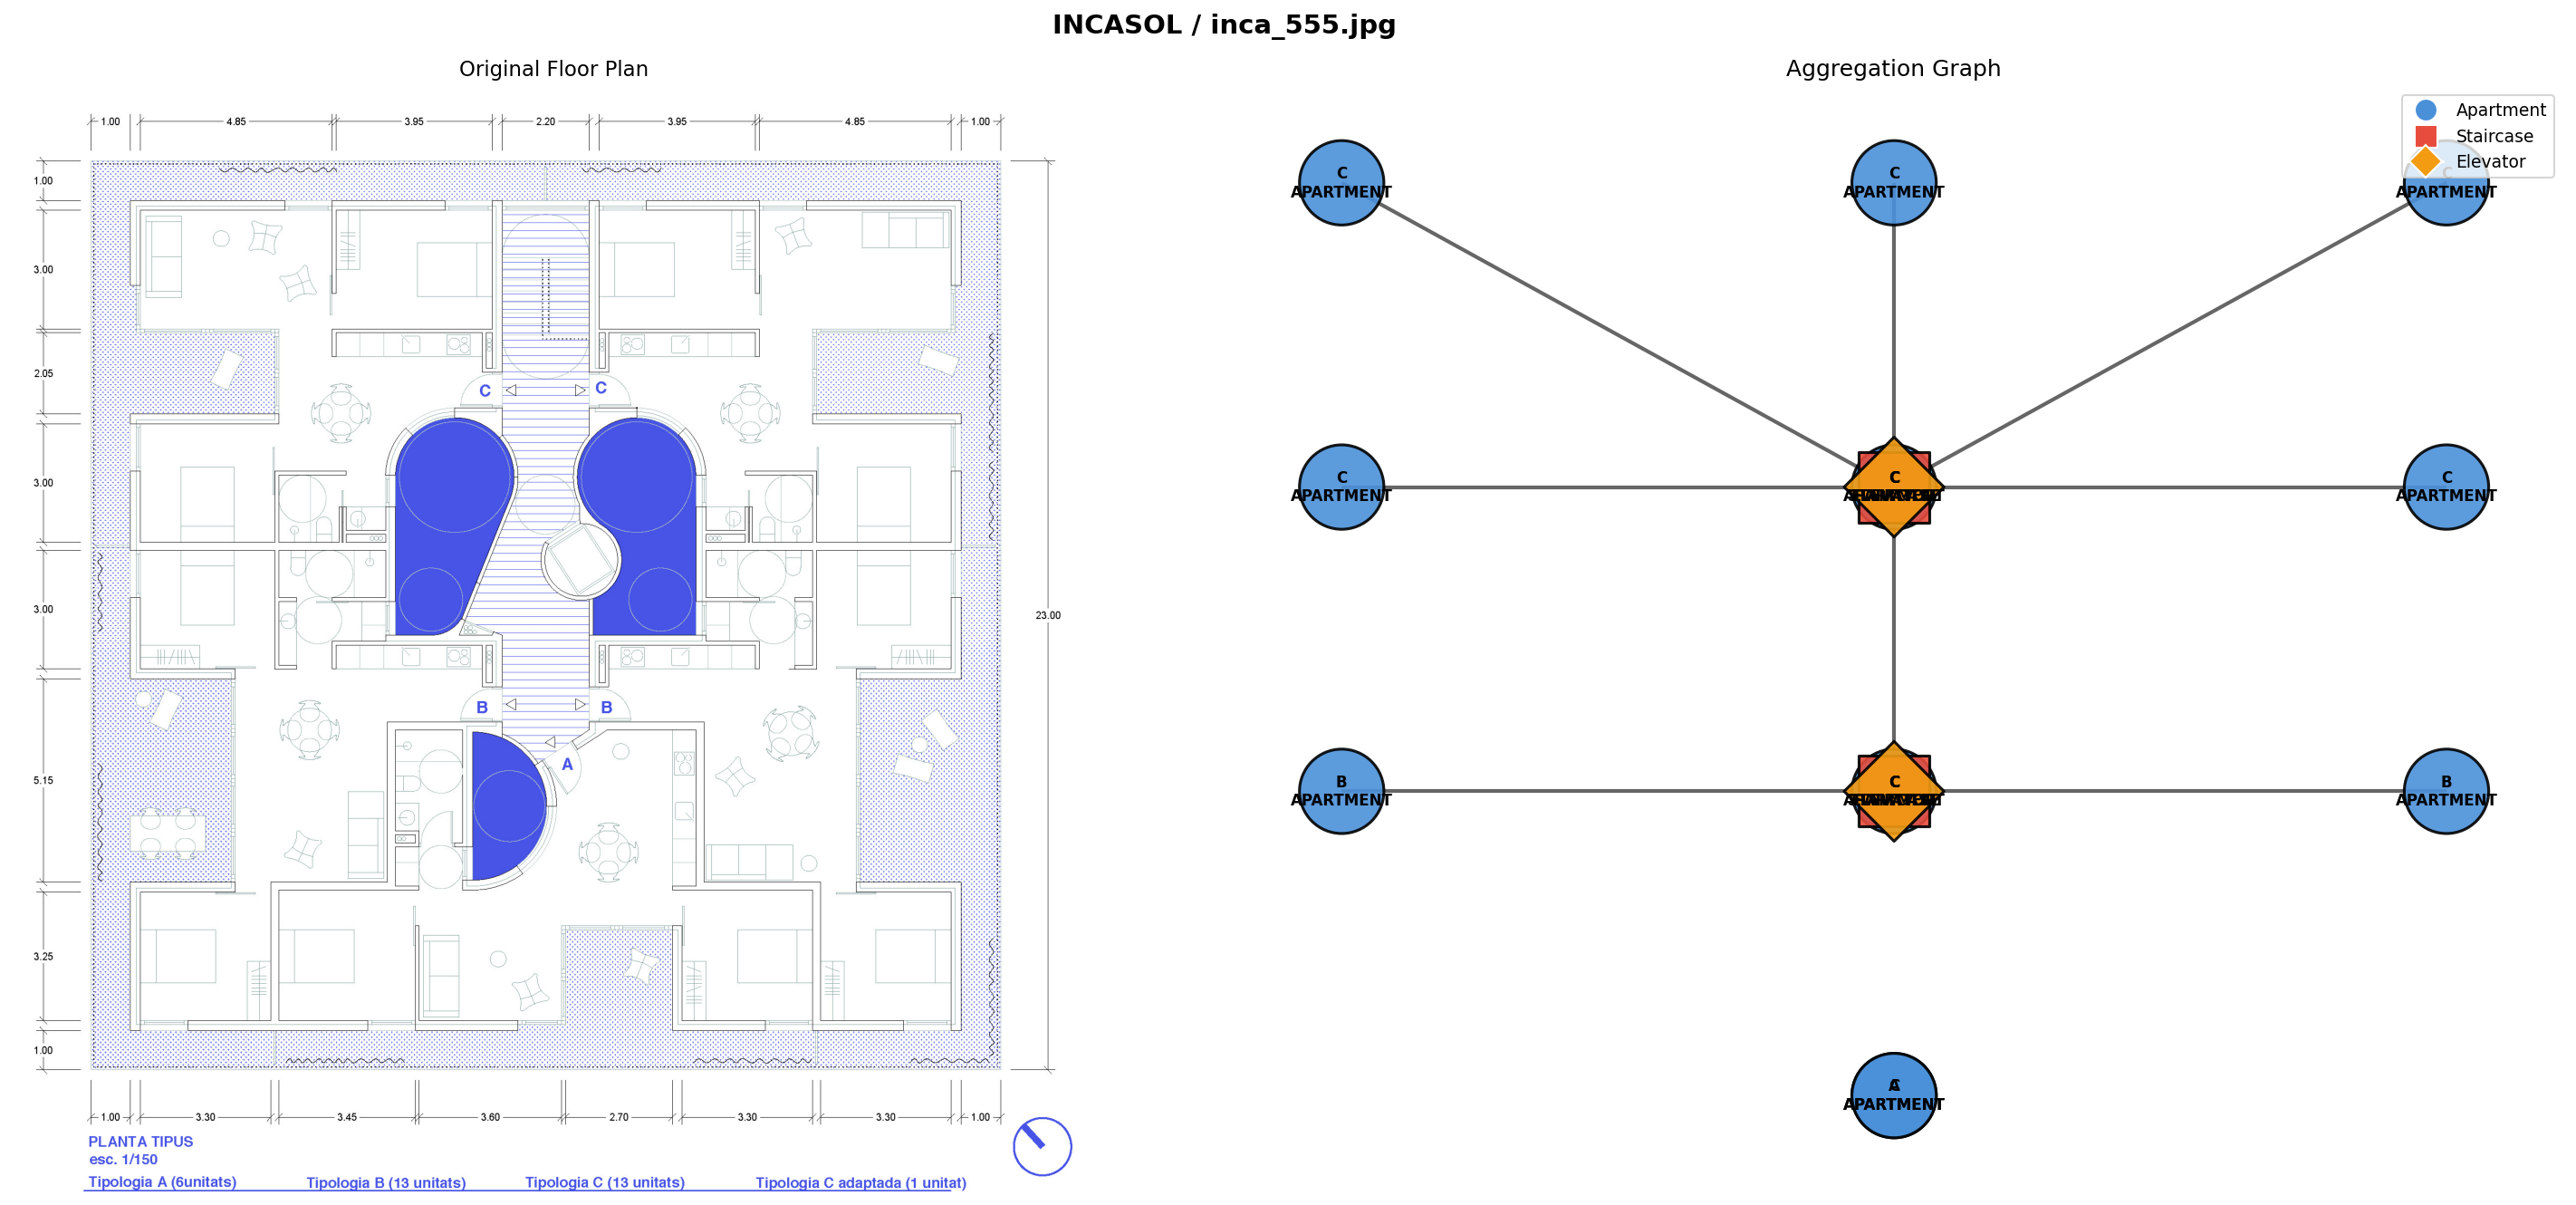
\includegraphics[width=\linewidth]{figures/examples/inca_555_aggregation.png}
    \caption{\textit{inca\_555.jpg} before review. The model over-counts the dwellings (eight apartments and two redundant cores) and leaves one apartment node disconnected, having interpreted the typology legend's unit totals as individual apartments.}
    \label{fig:inca_555}
\end{figure}

\begin{figure}[ht]
    \centering
    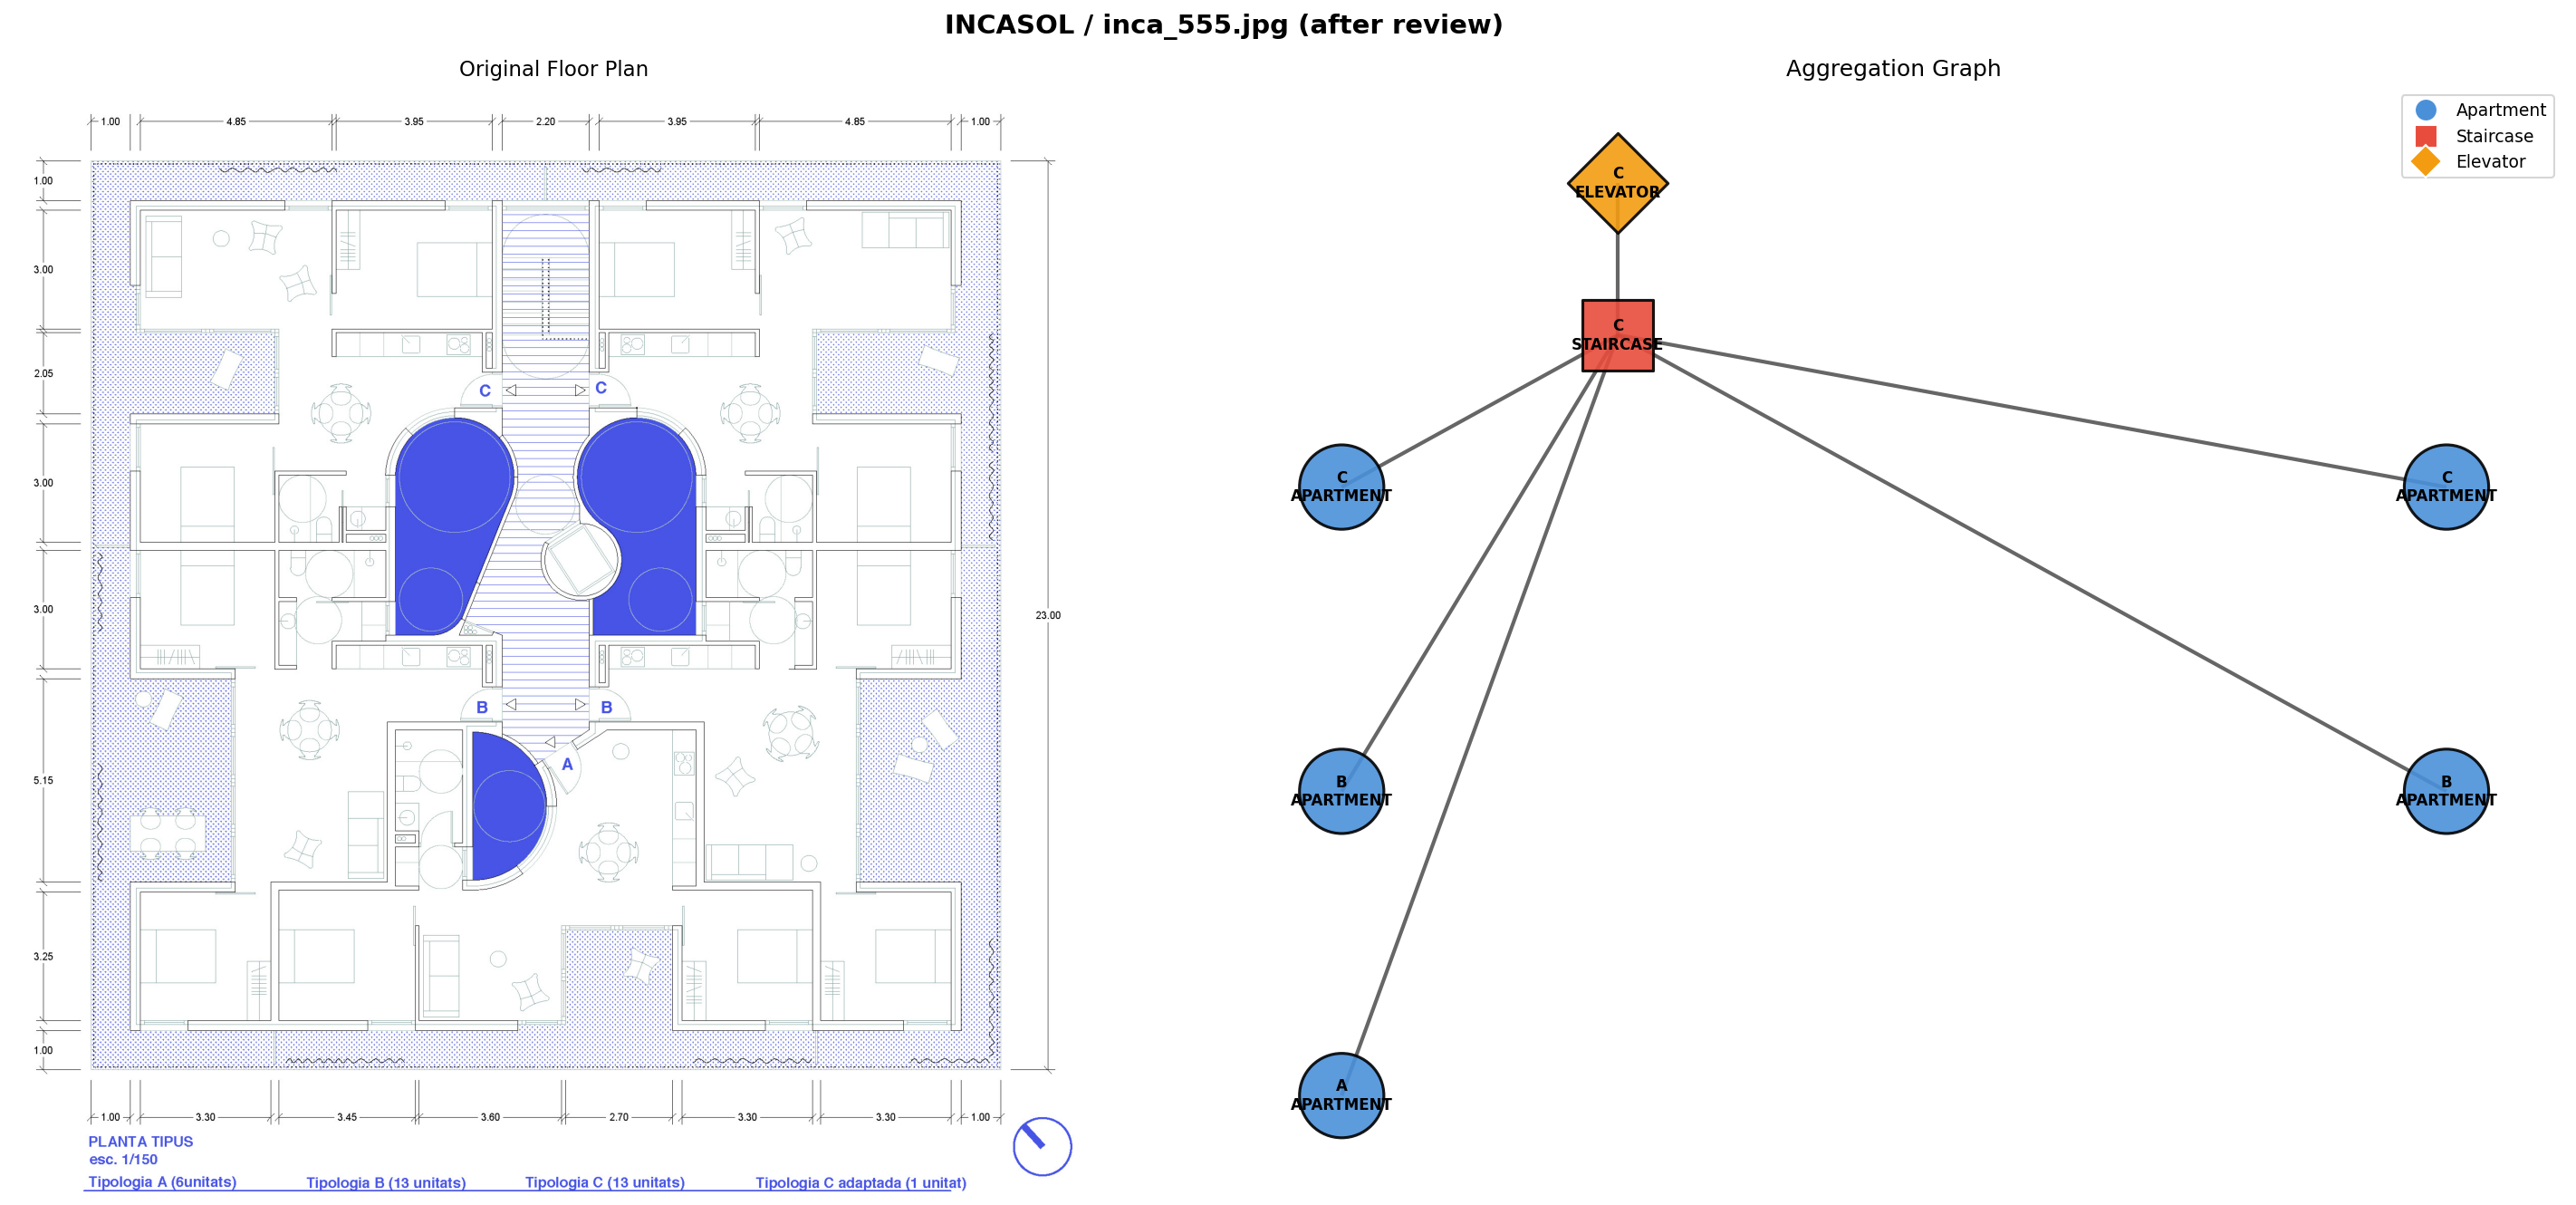
\includegraphics[width=0.7\linewidth]{figures/examples/inca_555_aggregation_reviewed.png}
    \caption{\textit{inca\_555.jpg} after human-in-the-loop review. The corrected graph contains the five true apartments (A, B, B, C, C) connected to a single staircase--elevator core, with no isolated nodes.}
    \label{fig:inca_555_reviewed}
\end{figure}


\section{3D Alignment (Step 6)}
\label{sec:exp-3d}

The final step assembles the 3D building graph and its visualisation. For the full corpus, the pipeline applies the default \emph{self-stacking} strategy: each 2D graph is replicated across three floors, and the staircase and elevator of consecutive floors are linked vertically to form the building's circulation core. This is the simplest way to obtain a 3D structure when only a single
representative floor plan is available, which is the common case in the dataset. Figure~\ref{fig:inca_555_3d} shows such a self-stacked building: a fully connected three-floor graph in which every floor is joined to the next through its staircase and elevator, and each apartment is placed in 3D according to the $(x, y)$ position predicted by the VLM, with the floor index as the vertical axis.

\begin{figure}[ht]
    \centering
    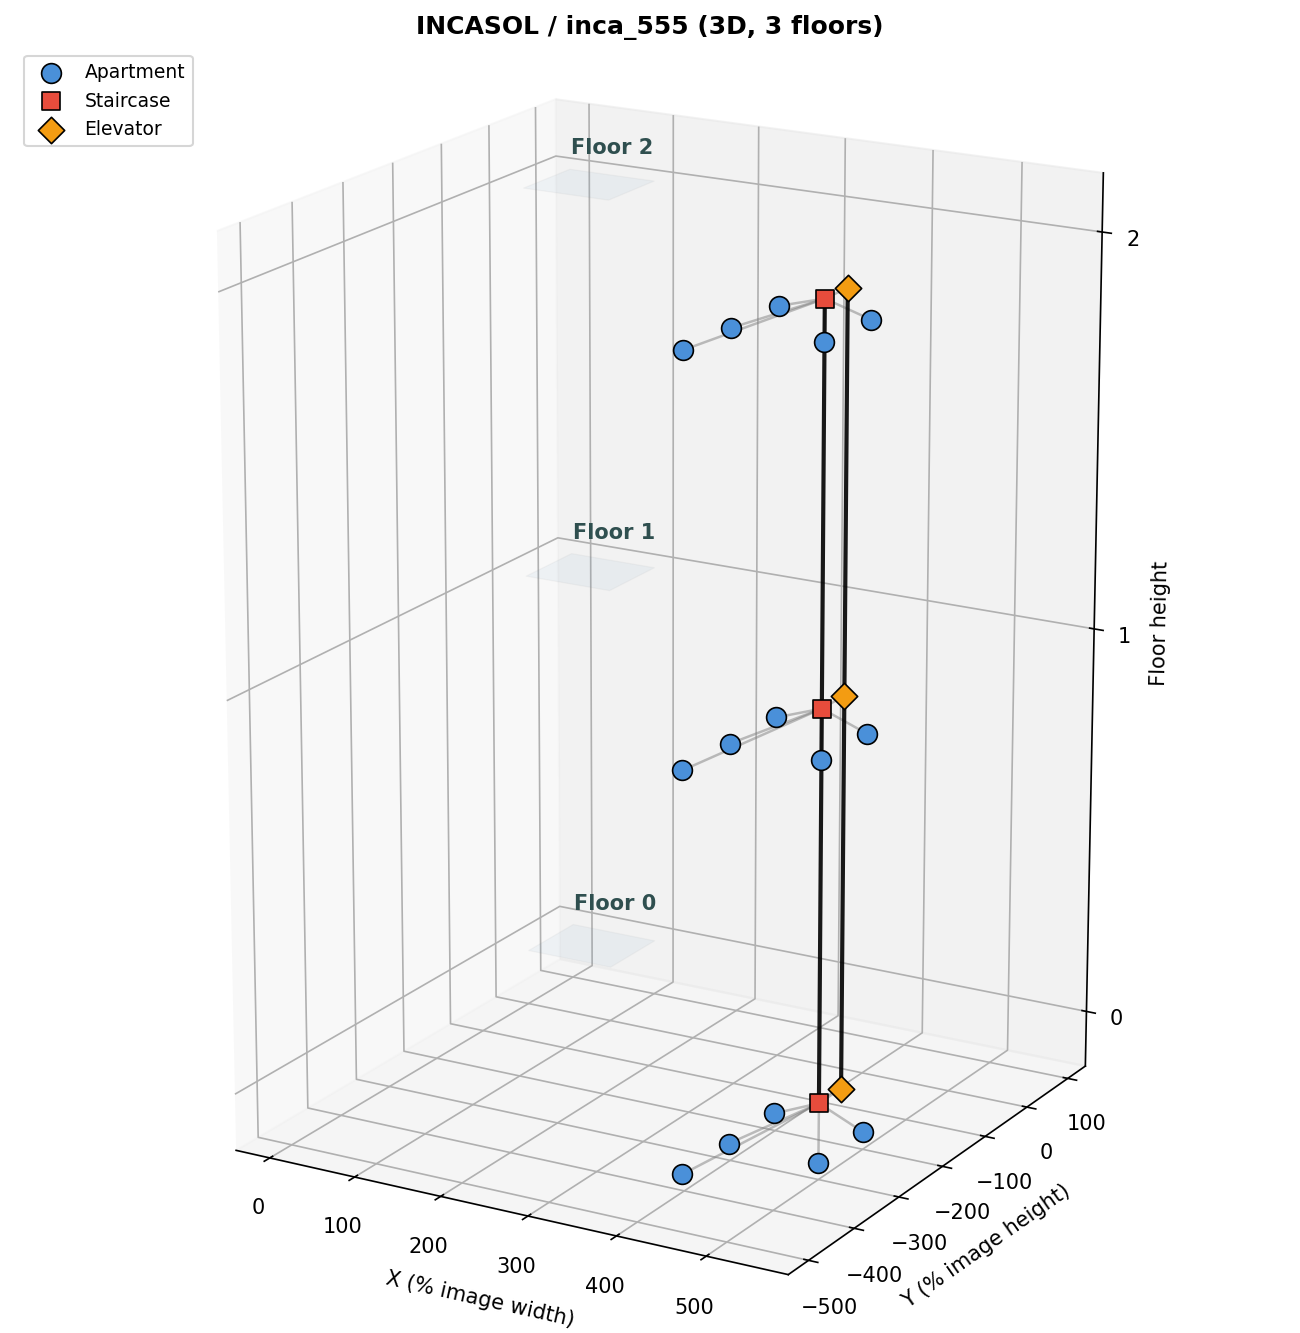
\includegraphics[width=0.45\linewidth]{figures/examples/inca_555_3d.png}
    \caption{Self-stacked 3D building graph for \textit{inca\_555.jpg}: the
    reviewed 2D floor replicated across three storeys, with the staircase and elevator linked vertically between consecutive floors. Apartment positions follow the VLM-predicted $(x, y)$ coordinates; the floor index forms the vertical axis.}
    \label{fig:inca_555_3d}
\end{figure}

Beyond this default behaviour, the same alignment routine also accepts a sequence of \emph{distinct} per-floor graphs, enabling true multi-floor assembly when separate floor plans of one building are available. To demonstrate this, the plans \textit{ibavi\_34} and \textit{ibavi\_35}---the ground floor (\textit{planta baixa}) and first floor (\textit{planta primera}) of the same building, sharing an identical apartment layout---were stacked into a single
two-floor graph (Figure~\ref{fig:ibavi_block_3d}). The two floors align correctly, with the shared staircase linking them vertically and each floor's apartments remaining connected only within their own level.

\begin{figure}[ht]
    \centering
    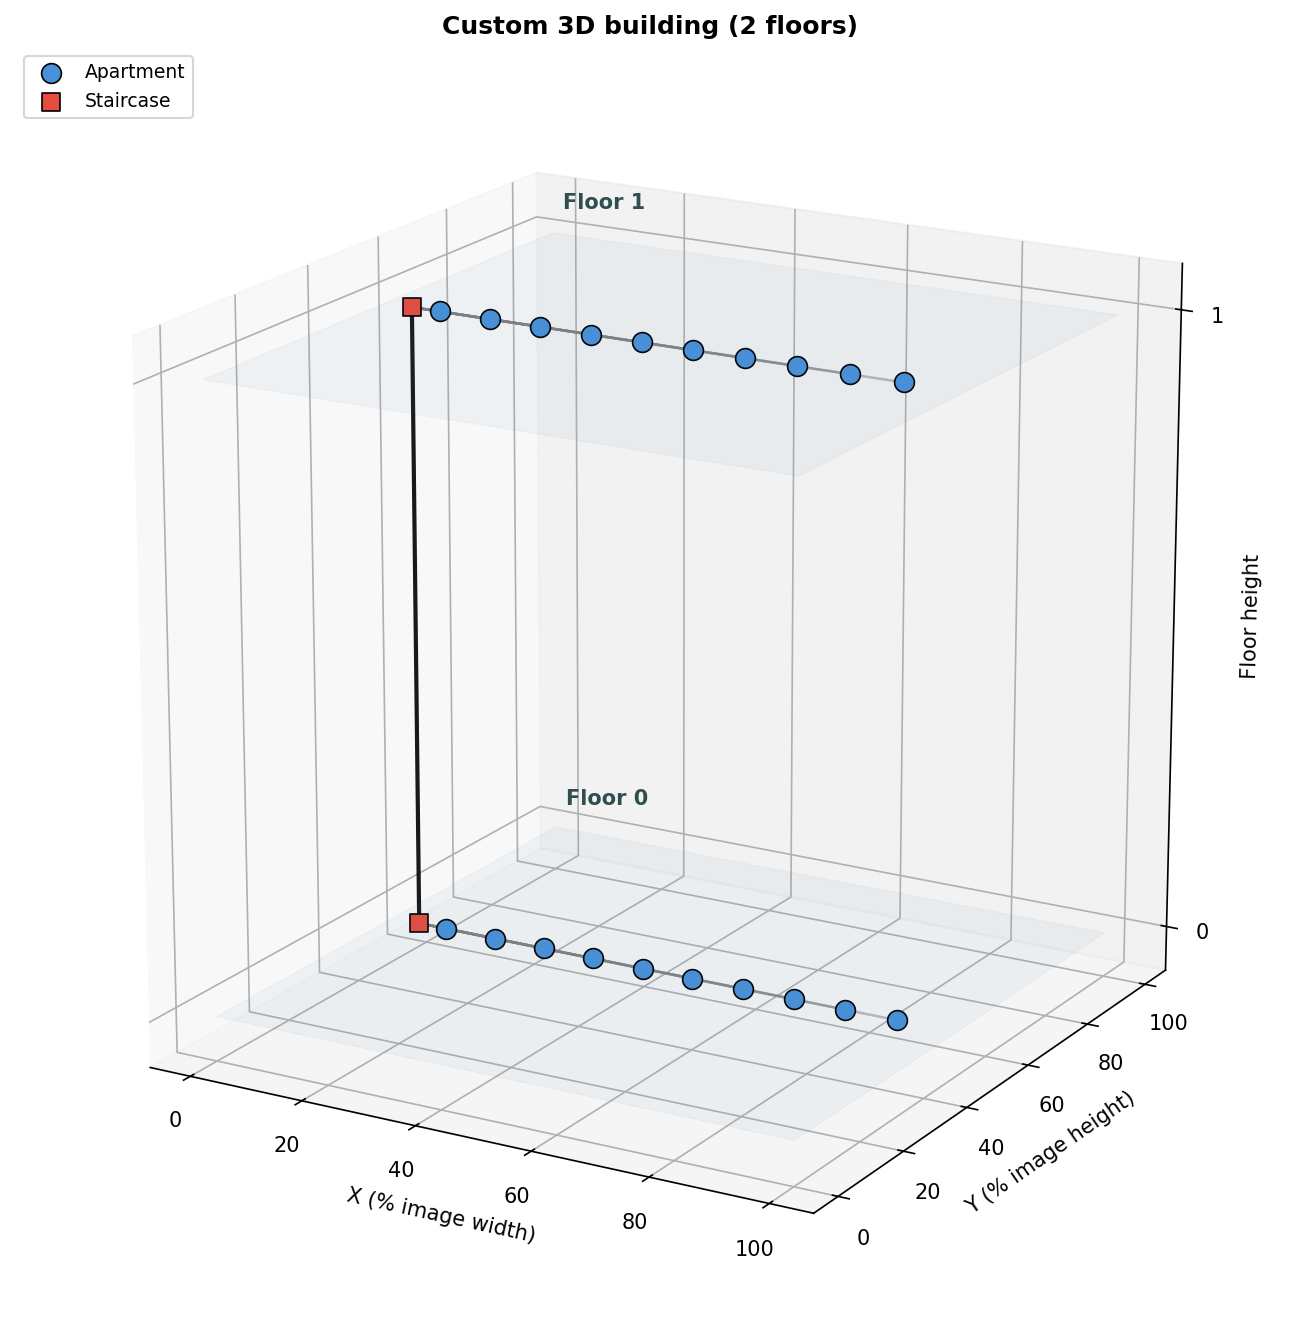
\includegraphics[width=0.4\linewidth]{figures/examples/ibavi_block_3d.png}
    \caption{Custom two-floor assembly of \textit{ibavi\_34} (ground floor) and
    \textit{ibavi\_35} (first floor) of the same building. The two manually
    corrected per-floor graphs are stacked and vertically linked through their
    shared staircase, demonstrating multi-floor alignment on distinct floors.}
    \label{fig:ibavi_block_3d}
\end{figure}


\section{Failure Mode Analysis}
\label{sec:exp-failure}

This section consolidates every observed failure mode into a single
view, grouped by \emph{root cause} rather than by pipeline step.
Table~\ref{tab:failure-modes} lists each mode, the stage it originates in, and the section in which it is quantified.

Two observations follow directly from this grouping. First, the failures separate cleanly into two families by where they originate: those rooted in \emph{classification} (typology catalogues and multi-floor sheets), in which a plan is wrongly admitted into extraction, and those rooted in \emph{extraction} (apartment counting, ambiguous circulation, coordinate imprecision, and the hard failures), which arise once an authetic aggregation plan is being processed.

Second, the no-fabrication edge rule determines how the extraction-rooted errors manifest: rather than inventing plausible-but-wrong connections, the model leaves uncertain links unmade, so its errors appear as conservative disconnections that the automated checks detect, rather than as silent topological corruption. The implications of these failure modes, and the directions they suggest for future work, are discussed in Chapter~\ref{ch:discussion}.

\begin{table}[ht]
\centering
\renewcommand{\arraystretch}{1.3}
\begin{tabular}{@{}p{6.0cm}cc@{}}
\toprule
\textbf{Failure mode} & \textbf{Root cause} & \textbf{Reported in} \\
\midrule
Typology catalogues classified as aggregation        & Step 1     & Sec.~\ref{sec:exp-classification} \\
Multi-floor sheets collapsed into one graph          & Step 1     & Sec.~\ref{sec:exp-extraction} \\
Apartment over- / under-counting                     & Steps 2--3 & Sec.~\ref{sec:exp-spotcheck} \\
Ambiguous vertical circulation (missed / hallucinated connector) & Step 2 & Sec.~\ref{sec:exp-extraction} \\
Coordinate imprecision / duplicate positions         & Step 2     & Sec.~\ref{sec:exp-extraction} \\
Hard extraction failures (no parseable graph)        & Step 2     & Sec.~\ref{sec:exp-extraction} \\
\bottomrule
\end{tabular}
\caption{The pipeline's failure modes, grouped by root cause. The errors themselves are quantified in the referenced sections; this table provides the cross-cutting view that the per-step analyses cannot.}
\label{tab:failure-modes}
\end{table}

% ============================================================
\chapter{Discussion \& Limitations}
\label{ch:discussion}

\section{Successes}

This project successfully addresses the problem it set out to solve: building a graph database of dwelling structures directly from raster floor plans using a Vision-Language Model---specifically the frozen \textbf{Qwen3-VL-8B-Instruct} model---and rendering the extracted structures as 3D building graphs from the generated \textit{JSON}. Crucially, this is achieved \emph{without any annotated training data and without fine-tuning the model}, which was the central constraint of the work: since no ground truth exists for the IBAVI, IMPSOL, and
INCASOL corpora, a supervised or fine-tuned approach was not viable, and a prompting-only pipeline proved a credible alternative.

The classification stage reaches an overall accuracy of 90.05\% over the 1,276 manually labelled plans (Section~\ref{sec:exp-classification}), with a weighted $F_1$ of 0.90, indicating reliable separation of the two principal classes. The extraction stage is similarly robust: of the 702 plans (predicted) routed into extraction, the model produced a parseable graph for 691, and 623 of those (90.2\%) pass all hard structural checks with a mean quality score of 0.924
(Section~\ref{sec:exp-extraction}). Taken together, these results show that a general-purpose VLM, driven only by prompt engineering, can convert the large majority of social-housing plans into well-formed topological graphs.

Beyond the headline accuracy, three design choices proved their value. First, decomposing the extraction into six focused sub-tasks kept each prompt simple and made failures \emph{localisable}---a wrong graph can be traced to the specific step that produced it, rather than to an opaque end-to-end model. Second, the no-fabrication edge rule ensured that the model's uncertainty surfaces as conservative, detectable disconnections rather than as silently invented connections, which is what makes the pipeline's output auditable by the automated checks and routable to human review. Third, the captured-reasoning fields (\code{building\_analysis}, \code{spatial\_analysis}) not only document each extraction for the manual spot-check but, in several cases, exposed an internal
inconsistency between the model's stated reasoning and its emitted graph---a useful diagnostic signal. Finally, the human-in-the-loop stage demonstrated that a single textual hint, persisted as visual memory, can correct a complex mis-extraction (Section~\ref{sec:exp-hitl}) without retraining the model.

\section{Limitations}

Despite these results, the approach has several limitations that bound the
strength of its conclusions.

\paragraph{Classification is the dominant bottleneck.} The most consequential
limitation is upstream of extraction: typology catalogues---sheets that present several unit \emph{types} side by side---are frequently misclassified as aggregation plans (Section~\ref{sec:exp-classification}), and multi-floor sheets that place two plans on one image are collapsed into a single graph. Because a plan wrongly admitted into extraction can never yield a correct graph, these
classification errors propagate downstream and account for most of the empty graphs and most of the human-review queue. This is a limitation of the single-image, single-floor assumption and of the classifier's difficulty in distinguishing a building floor from a catalogue of types.

\paragraph{The \textit{other} class is effectively unused.} Although the three-class scheme is conceptually necessary, the corpus contains only a single non-dwelling plan (Section~\ref{sec:exp-classification}). The \textit{other} category was therefore exercised too rarely to be evaluated meaningfully, and in practice the problem reduces to a near-binary one on this data. Correct non-residential plans are essentially absent from these social-housing archives.

\paragraph{Exact node-level fidelity remains imperfect.} On true aggregation plans, the model reliably produces \emph{well-formed} graphs but not always \emph{exact} ones: the spot-check (Section~\ref{sec:exp-spotcheck}) found apartment over- and under-counting to be the dominant residual error, especially on dense, radial, or legend-driven layouts where the model conflates per-type
unit totals with the number of drawn apartments. Vertical circulation is also occasionally misread, with elevators hallucinated or missed.

\paragraph{Validation relies on limited ground truth.} The absence of
annotations shapes not only the method but also its evaluation. Classification could be assessed exactly because the full corpus was hand-labelled, but extraction quality rests on a manual spot-check of roughly thirty plans by a single annotator; the resulting figures are an approximate lower bound rather than a corpus-wide measure, and they carry no inter-annotator agreement. Moreover, the ground-truth labels themselves are not infallible: both the exhaustive classification labelling and the spot-check were carried out by a
single annotator, so they may contain individual errors and reflect one interpreter's judgement on specific ambiguous cases---for example, plans on the boundary between a typology catalogue and a true aggregation, or sheets that combine a building floor with a unit-type detail. Without a second independent annotator these borderline decisions cannot be cross-validated, and a small number of labelling errors may therefore propagate into the reported metrics. The demonstrations of human-in-the-loop refinement and multi-floor 3D assembly are likewise based on individual examples rather than a large-scale study, so the generalisation of the persistent-memory mechanism across the dataset remains untested.


\paragraph{Constrained hardware and model scale.} The pipeline is bounded by the available hardware: the production model is the 8B variant on a single 24GB GPU, and the larger 30B Mixture-of-Experts variant could not be deployed (Section~\ref{sec:model_selection}). Some of the counting and disambiguation errors above are plausibly attributable to model scale, and a larger or reasoning-tuned model might reduce them---but this could not be verified within
the constraints of this work.

\paragraph{Coordinate imprecision.} Finally, node positions are estimated as percentage coordinates directly from the image, which is inherently imprecise: duplicate or out-of-range coordinates occur on a non-trivial fraction of graphs (Section~\ref{sec:exp-extraction}). This rarely affects the graph topology but degrades the geometric fidelity of the 3D visualisation.

% ============================================================
\chapter{Conclusion \& Future Work}
\label{ch:conclusion}

\section{Summary of Contributions}

This thesis set out to convert a corpus of unannotated Catalan social-housing floor plans into structured topological graphs, as the foundational data for future generative models of residential layout. In the absence of any ground truth---which rules out supervised training and fine-tuning---it pursued an annotation-free route built entirely on prompting a frozen Vision-Language Model. The work makes the following contributions.

\begin{itemize}
    \item \textbf{An annotation-free, prompting-only extraction pipeline.} A complete six-stage system was designed and implemented that takes a raster floor plan and produces a 2D access graph and a stacked 3D building graph,
    using a frozen \textbf{Qwen3-VL-8B-Instruct} model with no fine-tuning and no labelled training data. On the 1{,}276-plan corpus it classifies plans with 90.05\% accuracy and produces structurally valid graphs for the large majority of aggregation plans (90.2\% pass rate).

    \item \textbf{A decomposed, hybrid extraction methodology.} Rather than relying on a single monolithic Vision-Language Model (VLM) query, the pipeline is modularized into distinct sub-tasks. The inference-driven stages (classification, aggregation analysis, apartment detailing, and interactive review) are each governed by specialized prompts combining an expert architectural persona, explicit decision procedures, and visual in-context examples. Conversely, the validation strategy and structural stages (2D graph assembly and 3D alignment) are executed via strictly deterministic, prompt-free algorithms. This hybrid decomposition ensures that each VLM task remains computationally tractable and makes any extraction failures precisely attributable to a specific pipeline stage.

    \item \textbf{Design principles for trustworthy extraction.} Two choices in particular proved their value: the \emph{no-fabrication edge rule}, which makes the model's uncertainty surface as conservative, detectable disconnections rather than as silently invented connections; and the \emph{captured-reasoning fields}, which both document each extraction and expose inconsistencies between the model's stated reasoning and its emitted graph. Together they make the pipeline's output auditable.

    \item \textbf{A human-in-the-loop refinement with persistent visual memory.} An interactive stage allows an architect to correct a mis-extraction with a textual hint and reference crops that are persisted across sessions as few-shot examples, adapting the model's behaviour without any weight update.

    \item \textbf{An annotation-free validation strategy and an empirical study.} Lacking ground truth, the pipeline is evaluated through deterministic structural checks over the full corpus and a manual spot-check against the source images, complemented by an exhaustive manual classification labelling of all 1,276 plans. This yields the first quantitative characterisation of
    how a prompting-only VLM performs on this domain, including a clear analysis of its failure modes.
\end{itemize}

Overall, the work demonstrates that a general-purpose VLM, driven by prompt engineering alone, can transform the majority of social-housing plans into well-formed topological graphs, providing a practical and reproducible path to unlock an architectural archive that was previously locked inside raster images.

\section{Future Work}
\label{sec:future_work}

The limitations identified in Chapter~\ref{ch:discussion} point to several concrete directions for future research, ordered here from the most immediately actionable improvements to broader, exploratory applications.

\paragraph{Refining Taxonomic Classification.} Because misclassification is the dominant source of downstream extraction failure, the highest-value improvement lies directly upstream. Developing a dedicated detection class for \textit{typology catalogues}---which the current classifier frequently conflates with genuine aggregation plans---would significantly reduce the volume of non-spatial data erroneously routed into the extraction phase. Additionally, expanding the visual in-context examples for the under-represented \textit{other} class would improve the model's robustness against edge cases.

\paragraph{Multi-Plan Sheet Segmentation.} The current pipeline operates under the assumption of a single building floor per image. A dedicated pre-processing stage capable of detecting and segmenting architectural sheets that contain multiple distinct floor plans (e.g., ``P2--P4'' and ``P5--P8'' drawn on the same page) would allow each sub-plan to be extracted independently. These could then be spatially registered via the existing 3D-alignment routine, transforming a current failure mode into a robust multi-floor extraction capability.

\paragraph{Enhancing Node-Level Topological Fidelity.} Residual extraction errors are predominantly characterized by apartment miscounting on dense, radial, or legend-driven floor plans. Two avenues present strong potential here: first, increasing the Vision-Language Model's input resolution (\texttt{max\_pixels}) to ensure small labels and partition walls remain legible; and second, deploying a larger or natively reasoning-tuned VLM (e.g., 32B+ parameters), which the hardware constraints of this current work did not permit. Furthermore, implementing deterministic coordinate post-processing could automatically resolve duplicate or out-of-bounds spatial positions, directly enhancing the 3D visualization output.

\paragraph{Quantifying Human-in-the-Loop Efficacy.} While the persistent visual-memory mechanism was successfully demonstrated on localized edge cases, its longitudinal impact on subsequent inference runs remains unmeasured. A controlled ablation study---executing the pipeline both with and without the accumulated HITL feedback---would quantitatively determine whether the visual memory significantly improves zero-shot generalization to unseen plans, and at what threshold the in-context learning benefits saturate.

\paragraph{Expanding Ground-Truth Evaluation.} Introducing a second independent domain expert to annotate a subset of the dataset would establish a formal inter-annotator agreement baseline. This would place the classification metrics on firmer statistical ground and resolve ambiguous borderline cases (e.g., highly stylized typology catalogues). Expanding the qualitative spot-checks into a larger, exhaustively node- and edge-labelled subset would translate the current approximate lower bound of extraction quality into a mathematically precise error metric.

\paragraph{Closing the Generative AI Loop.} Ultimately, the core motivation of this thesis is to structure historical architectural data to feed downstream generative models. The natural progression of this research is to utilize the extracted \textit{JSON} database to train a graph-conditioned generative model (e.g., a GNN- or transformer-based layout synthesizer). Assessing whether the topological graphs extracted by this VLM pipeline possess sufficient fidelity to generate structurally valid, novel architectural layouts would definitively validate the foundational premise of this work.



% ============================================================
\printbibliography[heading=bibintoc, title={References}]

\begin{appendices}

\chapter{Code Availability}
\label{appendix:code}

The complete implementation of the pipeline described in this thesis is publicly
available as an open-source repository:

\begin{center}
\url{https://github.com/hangui11/floorplan-graph-vlm}
\end{center}

\noindent It contains the six pipeline modules (\code{src/step1\_classify.py}
through \code{src/step6\_stack3d.py}), the orchestrator (\code{src/pipeline.py}),
the prompt templates (\code{prompts/}), the evaluation scripts
(\code{eval\_classification.py}, \code{eval\_spotcheck.py}), and the pinned
dependencies (\code{requirements.txt}). Together with the deterministic
classification settings (Section~\ref{sec:reproducibility}), this enables the
experiments of Chapter~\ref{ch:experiments} to be reproduced end-to-end.


\chapter{Prompt Templates}
\label{appendix:prompting}

This appendix reproduces, verbatim, the four prompt templates used by the
VLM-driven steps of the pipeline. Placeholders in braces (\eg,
\code{\{apartment\_label\}}, \code{\{human\_hints\}}) are substituted at
runtime. The prompts are stored as plain-text files under \code{prompts/} so
they can be edited without redeploying the code.

\section{Classification (Step 1)}
\label{appendix:prompt-classify}

\begin{lstlisting}[style=prompt]
You are a professional architect specialized in residential building design and urban housing, with over 15 years of experience reading and producing technical drawings for Catalan and Spanish social housing projects (IBAVI, IMPSOL, INCASOL). You can tell at a glance whether a plan represents a whole building floor (aggregation of apartments around shared circulation), the internal layout of a single dwelling, or a drawing that is not a habitable dwelling at all (an office floor, retail/commercial locale, lobby, parking, technical/storage floor, or a pure circulation level). You are trained to ignore non-plan graphics such as elevations, sections, 3D renders, legends, area tables, and typology catalogs laid out side-by-side.

Look at this architectural floor plan image and classify it as ONE of the following three categories:

1. "aggregation" - A full building floor plan showing TWO OR MORE separate apartments/dwelling units within a single building envelope. These apartments are grouped around a shared element that belongs to the building (not to any single apartment): this shared element may be a corridor, a staircase core, an elevator, a central courtyard, an interior patio, a landing, a common room, or any circulation/communal space. Strong aggregation signals include:
   - Multiple apartment identifiers on the same plan such as "1A", "1B", "2A", "2B", "A", "B", "HA", "HB", "HABITATGE A", "HABITATGE B", "PIS 1", "PIS 2"...
   - Several kitchens (often labeled "Cuina", "C", "Cocina", "K") / bathrooms (labeled "Bany", "B", "Bano") / living areas repeated in different parts of the plan (one per apartment)
   - A building outline enclosing all apartments together
   - A shared courtyard, patio, atrium, or common area (labeled "Espai Comu", "pati", "patio", "courtyard") around which the apartments are distributed

2. "individual" - A plan showing ONE single apartment or dwelling unit, displaying only its internal rooms (bedrooms, kitchen, bathroom, living room, terrace...). It may be surrounded by a legend, area table, elevation, or 3D render, but only one housing unit floor plan is drawn. Strong individual signals include:
   - Exactly ONE kitchen visible in the whole plan
   - Exactly ONE living room / dining area visible
   - Bedrooms and bathrooms directly accessible through an internal corridor or distributor of the SAME apartment (not through a building corridor)
   - NO apartment identifiers such as "1A", "2B", "HABITATGE A" visible
   - NO shared building staircase core, NO elevator shaft, NO shared building corridor (a private internal staircase connecting two floors of a single duplex apartment does NOT break this rule)
   - A single continuous interior, even if it has multiple rooms separated by walls - walls between ROOMS of the same apartment do not make it an aggregation
   - The drawing may include decorative/artistic elements (landscape patterns, wind flows, shading, handwritten notes, title blocks, scale indications) around the plan - these are NOT shared spaces, they are annotations to be ignored

3. "other" - A plan that is NOT a habitable dwelling layout at all, and therefore contains NO dwelling units to extract. Use this category when the drawing shows none of the rooms that define a home (no kitchen AND no bathroom anywhere in the plan). Strong "other" signals include:
   - An office or workspace floor: open-plan desks, meeting/conference rooms, workstations, reception, no kitchen and no bathroom belonging to a dwelling
   - A retail or commercial locale ("local", "comercial", shop), a lobby/entrance hall ("vestibul", "hall"), or a community/technical room
   - A parking floor ("aparcament", "garatge"), a storage/technical level (machine rooms, installations), or a basement
   - A pure circulation level: only stairs, elevators, corridors and landings, with no dwelling attached
   - Note: a plan with shared stairs/elevators/corridor BUT no kitchens and no bathrooms is "other" - shared circulation alone does NOT make it "aggregation"; aggregation requires actual dwellings (each with its own kitchen and bathroom).

Important rules:
- If the image shows multiple apartment TYPOLOGY VARIANTS laid out side-by-side as separate detached drawings (e.g. "Type A" on the left, "Type B" on the right, each drawn inside its own rectangle without a shared wall or shared circulation between them), classify as "individual".
- If the apartments SHARE walls or SHARE circulation/courtyard within a single continuous building footprint, classify as "aggregation" - even if only a staircase or only a courtyard is visible as the shared element.
- Plans featuring a shared central courtyard with apartments drawn around its four sides are "aggregation".
- Ignore elevation views, 3D renders, section cuts, scale bars, decorative artwork, wave/wind patterns, landscape drawings, handwritten notes, and legends when deciding.

Disambiguation - common confusions to avoid:
- Walls between ROOMS of a single apartment (e.g. walls separating a bedroom from a bathroom) do NOT make the plan an aggregation. Aggregation requires MULTIPLE SELF-CONTAINED apartments, each with its own kitchen and bathroom.
- Empty internal space inside a single apartment (a living room, a distributor, a vestibule) is NOT a shared corridor. A shared corridor runs BETWEEN apartments and gives access to MORE THAN ONE front door.
- Curved fans, shaded patterns, or decorative shapes inside or around the plan are drawing annotations, NOT courtyards. A real courtyard is an enclosed open-air space with apartments drawn on at least two of its sides.

Decision procedure (follow in order):
1. Count the kitchens ("Cuina"/"C"/"Cocina"/"K") AND the bathrooms ("Bany"/"B"/"Bano") in the whole plan. If there are ZERO kitchens AND ZERO dwelling bathrooms (e.g. an office, parking, or pure circulation level) -> "other". Shared stairs/elevators/corridors without any dwelling do NOT change this.
2. If there is at least one kitchen, check the count. If you see exactly ONE kitchen in the whole plan, regardless of the number of bathrooms -> "individual".
3. Look for repeated apartment identifiers ("1A/1B", "A/B", "HABITATGE A/B"). If none are present, and there is only one main living area -> most likely "individual".
4. Only if the plan shows multiple kitchens, multiple self-contained units, AND a shared element (corridor, stair core, courtyard, landing) connecting them -> "aggregation".

Execute the 4-step decision procedure silently. Answer with ONLY one word: aggregation, individual, or other
\end{lstlisting}

\section{Aggregation Analysis (Step 2)}
\label{appendix:prompt-aggregation}

\begin{lstlisting}[style=prompt]
You are a professional architect specialized in residential building layouts, with deep familiarity with Catalan/Spanish social housing plans and their conventional symbols (door arcs, stair treads, elevator shafts) and Catalan room abbreviations (H, EMC, SC, B, Te, P...).

You are analyzing an aggregation floor plan - a full building floor showing multiple apartments arranged around shared circulation spaces.

Your task is to identify and extract the macro-structure of this building floor as a spatial graph. Identify the following nodes:

1. **Each individual apartment/housing unit** - these are separate dwellings, each with its own front door (the principal entrance door from the shared corridor/hallway into the private apartment). Each apartment becomes a node in the graph.
2. **All staircases** - shown as parallel diagonal lines (stair treads) or labeled with stair symbols. These are vertical circulation elements shared by the building.
3. **All elevators** - shown as a rectangular shaft, often with an "X" pattern, a circle, or labeled. These are vertical circulation elements shared by the building.

For each element found, provide:

For apartments:
- node_id: sequential integer starting at 0
- type: "apartment"
- label: the label/letter visible on the plan (e.g. "A", "B", "HA", "HB", "HABITATGE A"), or null
- door_position: approximate [x, y] as percentage of image dimensions where the principal entrance door of this apartment is located (the door connecting to the shared corridor/hallway)

For staircases:
- node_id: sequential integer (continuing from apartments)
- type: "staircase"
- label: any visible label, or null
- position: approximate [x, y] as percentage of image dimensions

For elevators:
- node_id: sequential integer (continuing)
- type: "elevator"
- label: any visible label, or null
- position: approximate [x, y] as percentage of image dimensions

Graph Edge Rules (How to connect nodes):
- Create a clean "hub-and-spoke" network topology where vertical circulation nodes act as hubs.
- Connect each apartment to the vertical circulation that serves it via the shared corridor/landing. If both a staircase and an elevator share the same core/landing, connect the apartment to BOTH - they are part of one circulation core.
- Do NOT draw edges directly between two apartments. Apartments do not connect to each other.
- Connect a staircase node to an elevator node if they are adjacent or open onto the same landing. A staircase and an elevator in the same core must NOT be left as separate disconnected components.
- The whole graph should form a single connected component: do not leave a connector (especially the elevator) isolated when it clearly belongs to the shared core.
- IMPORTANT - only create an edge you can actually trace on the plan. If an apartment's connection to the shared circulation is not visible, leave it unconnected rather than guessing: a missing edge is better than an invented one. Do NOT fabricate a connection just to link every node.

Return ONLY a valid JSON object matching this exact schema layout:
{
  "building_analysis": "string - Briefly describe the overall spatial arrangement of the building floor (e.g., 'Central stair and elevator core serving 4 perimeter apartments' or 'Linear corridor layout with a staircase at the east end serving 3 units') to anchor visual attention before outputting coordinates.",
  "nodes": [
    {"node_id": 0, "type": "apartment", "label": "A", "door_position": [25, 30]},
    {"node_id": 1, "type": "apartment", "label": "B", "door_position": [75, 30]},
    {"node_id": 2, "type": "staircase", "label": null, "position": [50, 50]},
    {"node_id": 3, "type": "elevator", "label": null, "position": [52, 50]}
  ],
  "edges": [
    {"from_node_id": 0, "to_node_id": 2},
    {"from_node_id": 1, "to_node_id": 2},
    {"from_node_id": 2, "to_node_id": 3}
  ]
}
\end{lstlisting}

The canonical aggregation plan \code{inca\_05.jpg} is supplied as a one-shot
visual example, paired with its expected JSON output (six apartments around a
central core with one staircase and two elevators), teaching the model both the
visual pattern and the response schema simultaneously.

\section{Apartment Detailing (Step 3)}
\label{appendix:prompt-details}

The placeholders \code{\{apartment\_label\}}, \code{\{x\}}, and \code{\{y\}} are
filled with the label and approximate position of the apartment under
inspection, isolating one apartment per call.

\begin{lstlisting}[style=prompt]
You are a professional architect specialized in residential building layouts, with deep familiarity with Catalan/Spanish social housing plans and their conventional room abbreviations (H/D = bedroom, EMC/SC = living-kitchen, B/CH = bathroom, Te/T/Jh = terrace, P/Db = corridor...).

You are analyzing an aggregation floor plan that contains multiple apartments.
Focus ONLY on the apartment labeled "{apartment_label}" (located approximately at position [{x}, {y}] as a percentage of image dimensions).

Your task is to identify the boundary walls of THIS single apartment and extract its internal room composition based on the visible labels.

Important Extraction Rules:
- Count ONLY rooms strictly enclosed within the boundary walls of apartment "{apartment_label}". Do not count rooms belonging to neighboring apartments or shared corridors.
- "EMC" / "SC" / "S-C" indicate a combined Living-Kitchen space. If you see "EMC", count it as 1 kitchen AND 1 living_room, but treat it as a single enclosed space when calculating total_rooms.
- If you cannot clearly see the interior of this apartment, set all counts to 0 and room_labels to [].

Field notes (read before filling the JSON):
- "spatial_analysis": briefly state where this apartment is located and identify its surrounding walls to prevent counting neighboring rooms.
- "num_bedrooms": count of bedrooms (H, H1, H2, D, D1, dormitori, habitacio...).
- "num_bathrooms": count of bathrooms/toilets (B, CH, bany, WC...).
- "num_kitchens": count of kitchens (K, C, cuina) AND combined spaces (EMC, SC).
- "num_living_rooms": count of living/dining rooms (E, EM, S, estar, menjador) AND combined spaces (EMC, SC).
- "num_terraces": count of terraces, balconies, winter gardens (Te, T, Jh, Px, Po, terrassa, balco).
- "has_corridor": true if there is an internal distributor (P, Db, Ds, passadis), otherwise false.
- "total_rooms": total count of physical enclosed rooms inside this apartment.
- "room_labels": the exact labels visible inside this apartment.

Return ONLY a valid JSON object matching this exact schema (the values below are concrete examples of the correct TYPE, not text to copy):
{
  "spatial_analysis": "Apartment B is in the lower-left quadrant, bounded by the central corridor to the north and the building wall to the west.",
  "num_bedrooms": 2,
  "num_bathrooms": 1,
  "num_kitchens": 1,
  "num_living_rooms": 1,
  "num_terraces": 1,
  "has_corridor": true,
  "total_rooms": 5,
  "room_labels": ["H1", "H2", "EMC", "B", "Te"]
}

Execute the spatial analysis silently inside the JSON. Do NOT wrap the output in markdown code blocks. Output ONLY the raw JSON brackets.
\end{lstlisting}

\section{Human-in-the-Loop Re-extraction (Step 5)}
\label{appendix:prompt-review}

The placeholder \code{\{human\_hints\}} is replaced with the architect's
free-text hint(s); reference crops of staircases/elevators, when available, are
prepended as few-shot visual examples.

\begin{lstlisting}[style=prompt]
You are a professional architect specialized in residential building layouts, with deep familiarity with Catalan/Spanish social housing plans and their conventional symbols for vertical circulation (stair treads drawn as parallel segments, elevator shafts drawn as small squares with an X or an inscribed circle).

You previously analyzed this aggregation floor plan and did NOT identify any staircase or elevator. However, an architectural aggregation block normally has at least one shared vertical circulation element (staircase and/or elevator) used by the apartments.

IMPORTANT: The images provided BEFORE the main floor plan (if any) are REFERENCE examples showing exactly how a staircase or an elevator is drawn in this dataset. Use those examples to recognize the same visual pattern inside the current floor plan. The LAST image in the sequence is the floor plan you must re-analyze.

A HUMAN reviewer has confirmed the following hints about this plan:
{human_hints}

Please re-examine the image carefully, paying special attention to:

1. Staircase symbols - Look for parallel diagonal lines or rectangles drawn as a series of equally-spaced parallel segments, a rectangle divided into narrow strips (often with an arrow indicating ascent), or U-shaped parallel rectangles. Look for labels like "E", "ES", "ESC", "escala", "HA", "HB".
2. Elevator symbols - Look for a small square/rectangle with an "X" diagonal cross inside, a square with a circle inscribed in it, or labels like "A", "AS", "ASC", "ascensor", "lift".
3. Placement - Staircases/elevators are usually in a central location adjacent to a shared corridor serving multiple apartments, or grouped together in a "core".

Now, please generate the FULL aggregation graph again, including apartments, staircases, and elevators.

Graph Edge Rules (How to connect nodes):
- Create a clean "hub-and-spoke" network topology where vertical circulation nodes act as hubs.
- Connect each apartment to the vertical circulation that serves it via the shared corridor/landing. If both a staircase and an elevator share the same core/landing, connect the apartment to BOTH (they are part of one circulation core).
- Connect the staircase and the elevator to each other when they sit in the same core or open onto the same landing. A staircase and an elevator in the same core must NOT be left as separate disconnected components.
- Do NOT draw edges directly between two apartments.
- The whole graph must form a SINGLE connected component: every apartment and every connector must be reachable from every other through the core. Do not leave any node (especially the elevator) isolated.
- Only create an edge you can actually trace on the plan. If an apartment's connection to the shared circulation is genuinely not visible after re-examination, leave it unconnected rather than guessing: a missing edge is better than an invented one.

Field notes (read before filling the JSON):
- "building_analysis": acknowledge the human hints and briefly describe exactly where you found the previously missed vertical circulation, to anchor your visual attention before outputting coordinates.
- "no_connector_confirmed": include this key with the literal value true ONLY if, after this careful re-examination and reading the human hints, you are absolutely certain the plan has NO staircase or elevator visible. Otherwise OMIT the key entirely (do not set it to false, do not write a sentence as its value).

Return ONLY a valid JSON object matching this exact schema layout (note the values below are concrete examples of the correct TYPE, not text to copy):
{
  "building_analysis": "Found the staircase in the central core between apartments A and B, as the reviewer indicated.",
  "nodes": [
    {"node_id": 0, "type": "apartment", "label": "A", "door_position": [25, 30]},
    {"node_id": 1, "type": "staircase", "label": null, "position": [50, 50]}
  ],
  "edges": [
    {"from_node_id": 0, "to_node_id": 1}
  ]
}

Execute the analysis silently inside the JSON. Do NOT wrap the output in markdown code blocks. Output ONLY the raw JSON brackets.
\end{lstlisting}


% ============================================================
\chapter{In-Context Examples}
\label{appendix:examples}

This appendix documents the visual in-context (few-shot) examples supplied to the VLM-driven steps that use them (Steps~1, 2, and~5). The example assets are committed alongside the source code so that every run sees identical examples. To avoid circular reference, an example is skipped whenever the target image is the example itself. Step~3 is zero-shot (no reference image), and Steps~4 and~6 are deterministic and use no VLM.

\section{Classification (two-shot)}
\label{appendix:ex-classify}

The classification prompt is preceded by two reference plans (Figure \ref{fig:ex-agg}), one per extractable class, each carrying the caption quoted below.

\begin{figure}[ht]
\centering
\begin{minipage}[t]{0.47\textwidth}
  \centering
  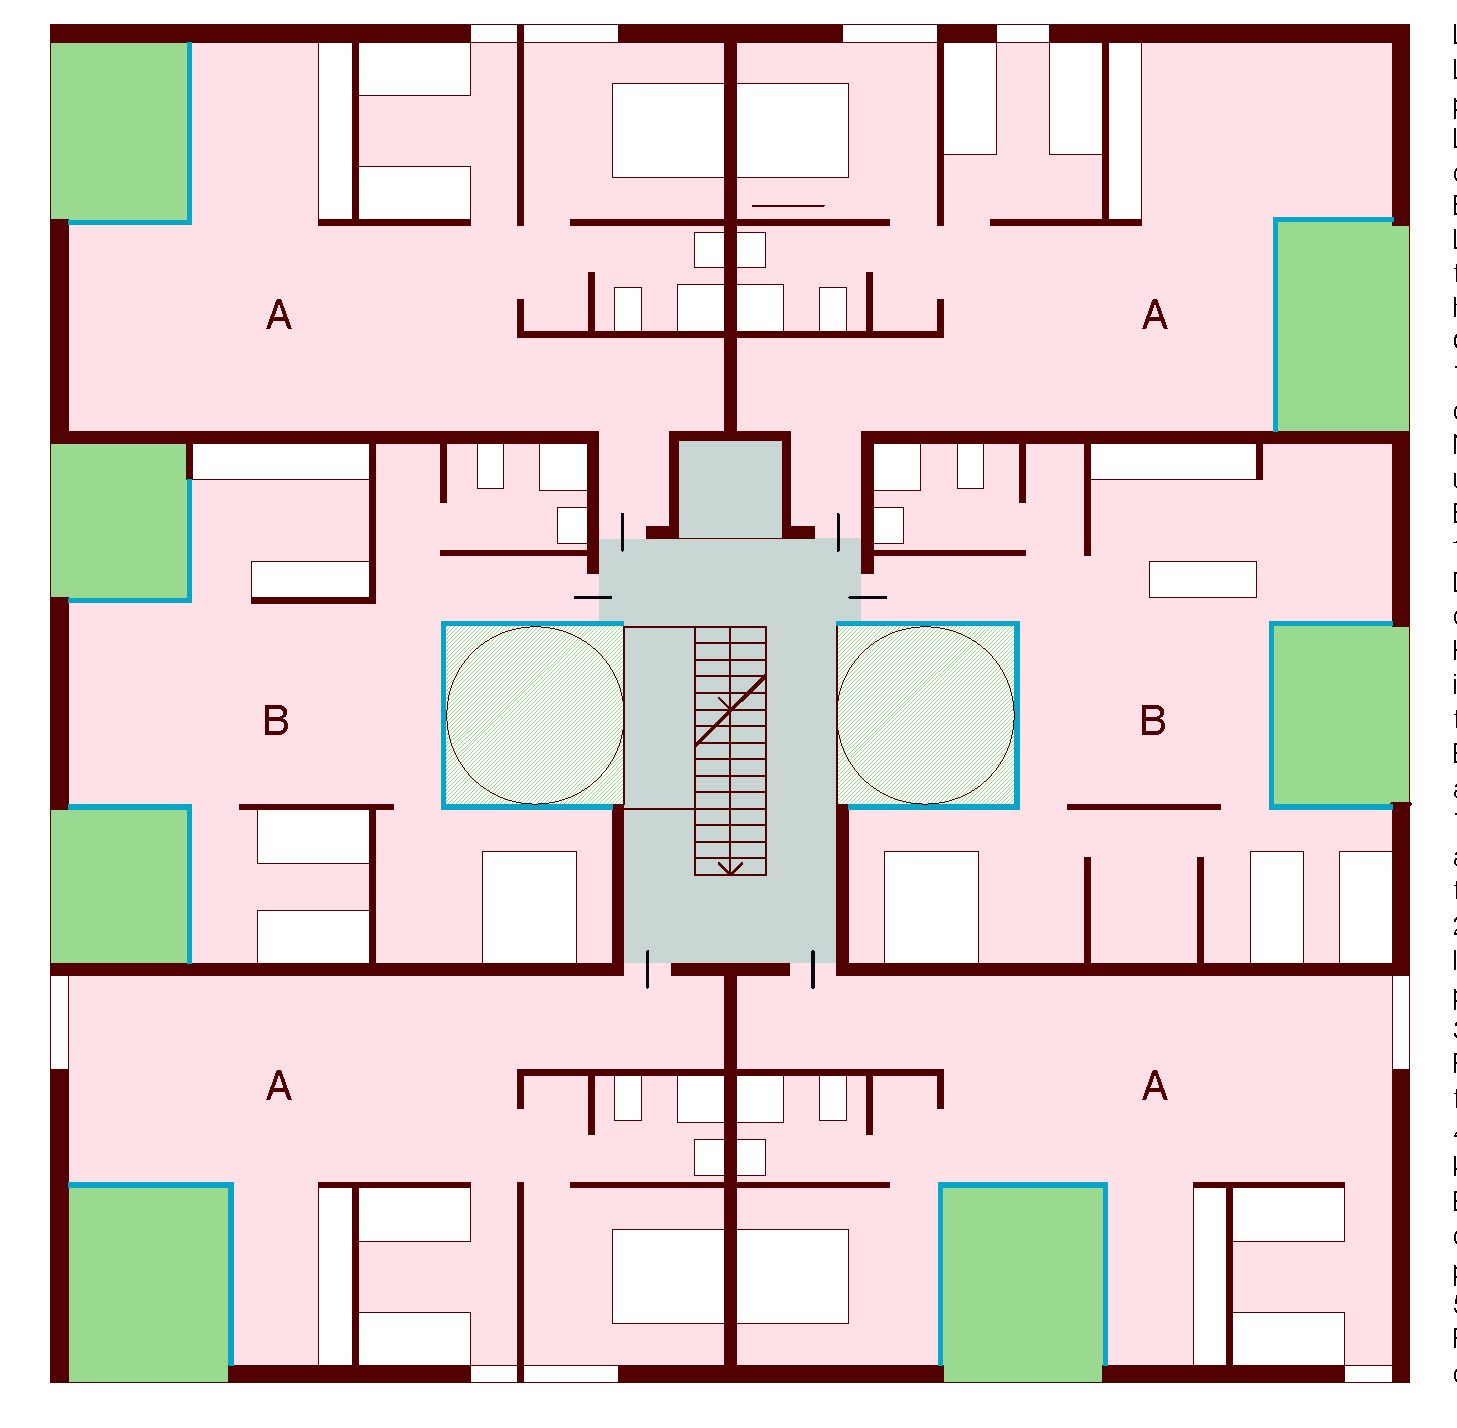
\includegraphics[width=\linewidth]{figures/examples/inca_05.jpg}
  \par\smallskip
  {\footnotesize\itshape ``Reference example --- this plan is an AGGREGATION:
  multiple apartments (labeled A, A, B, B) arranged around a shared central core
  with a staircase and two elevators.''}
\end{minipage}\hfill
\begin{minipage}[t]{0.47\textwidth}
  \centering
  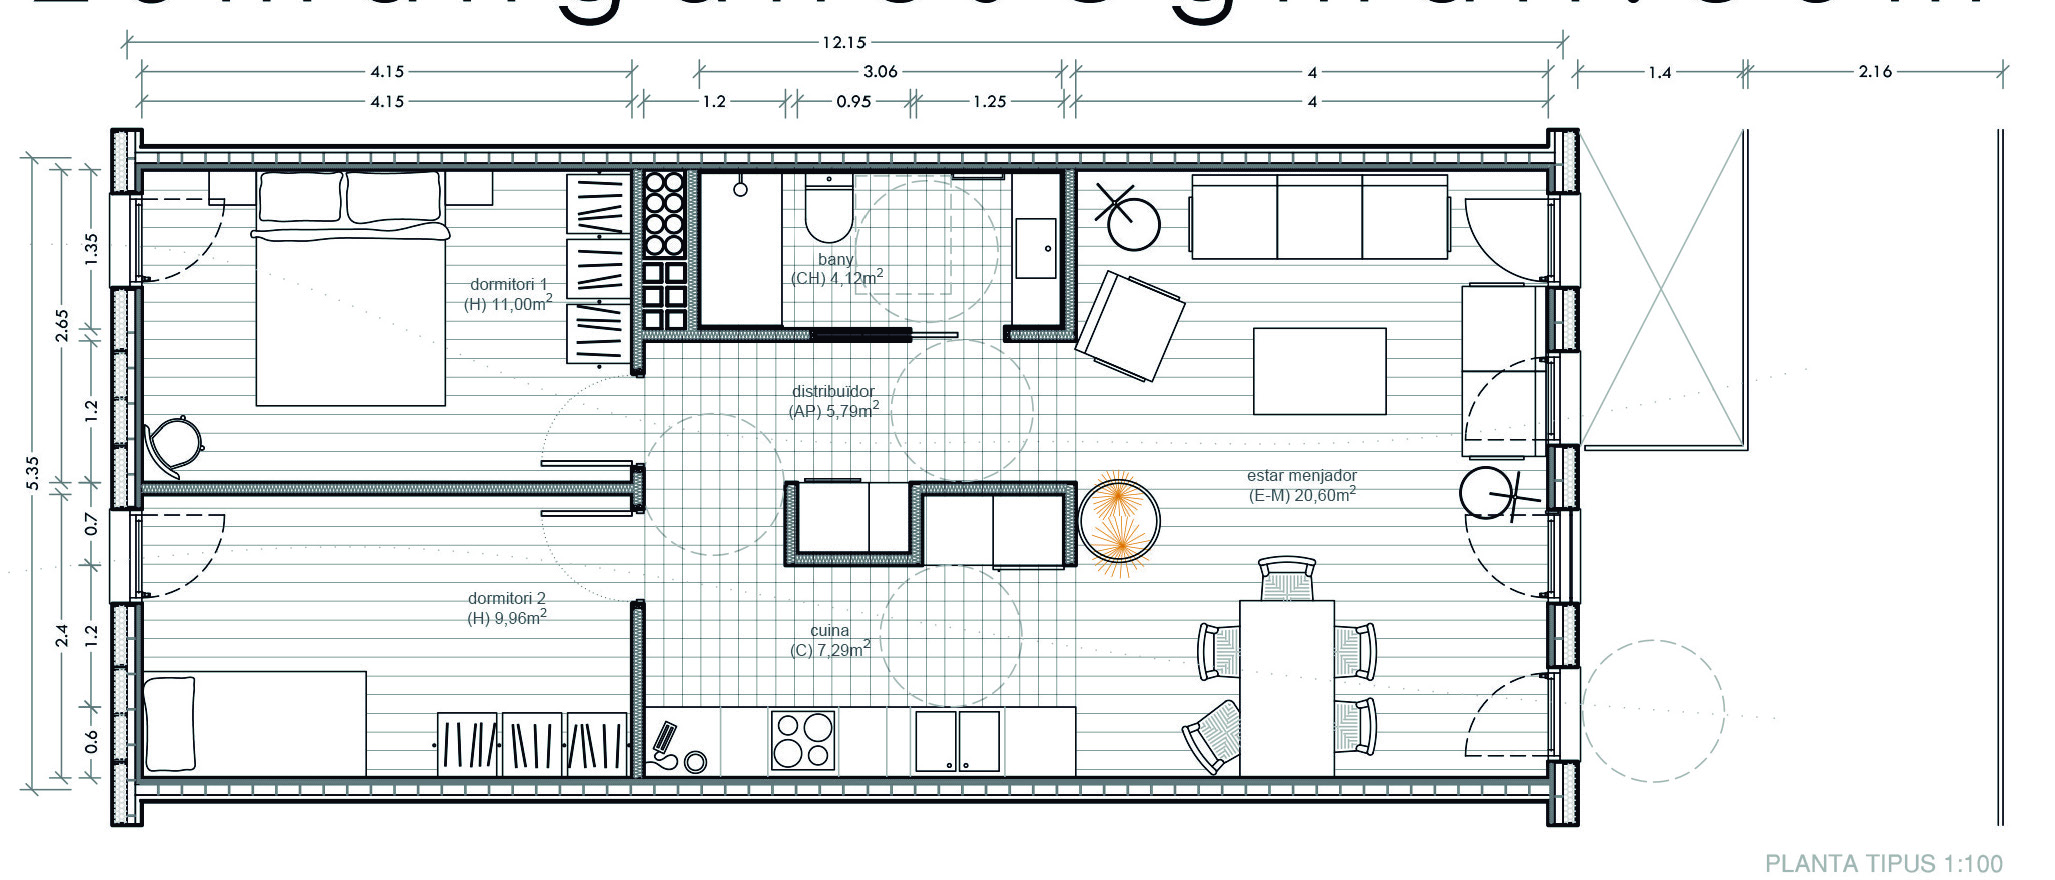
\includegraphics[width=\linewidth]{figures/examples/inca_50.jpg}
  \par\smallskip
  {\footnotesize\itshape ``Reference example --- this plan is an INDIVIDUAL
  apartment: a single dwelling with one kitchen (cuina), one bathroom (bany),
  one living-dining (estar menjador), and two bedrooms (dormitori).''}
\end{minipage}
\caption{Two-shot visual examples prepended to the Step~1 classification
prompt: \code{inca\_05.jpg} (aggregation, left) and \code{inca\_50.jpg}
(individual, right).}
\label{fig:ex-classify}
\end{figure}

\section{Aggregation Analysis (one-shot)}
\label{appendix:ex-aggregation}

The aggregation prompt receives a single canonical plan (Figure~\ref{fig:ex-agg})
paired with its expected JSON output, teaching the visual pattern and the
response schema simultaneously.

\begin{figure}[ht]
\centering
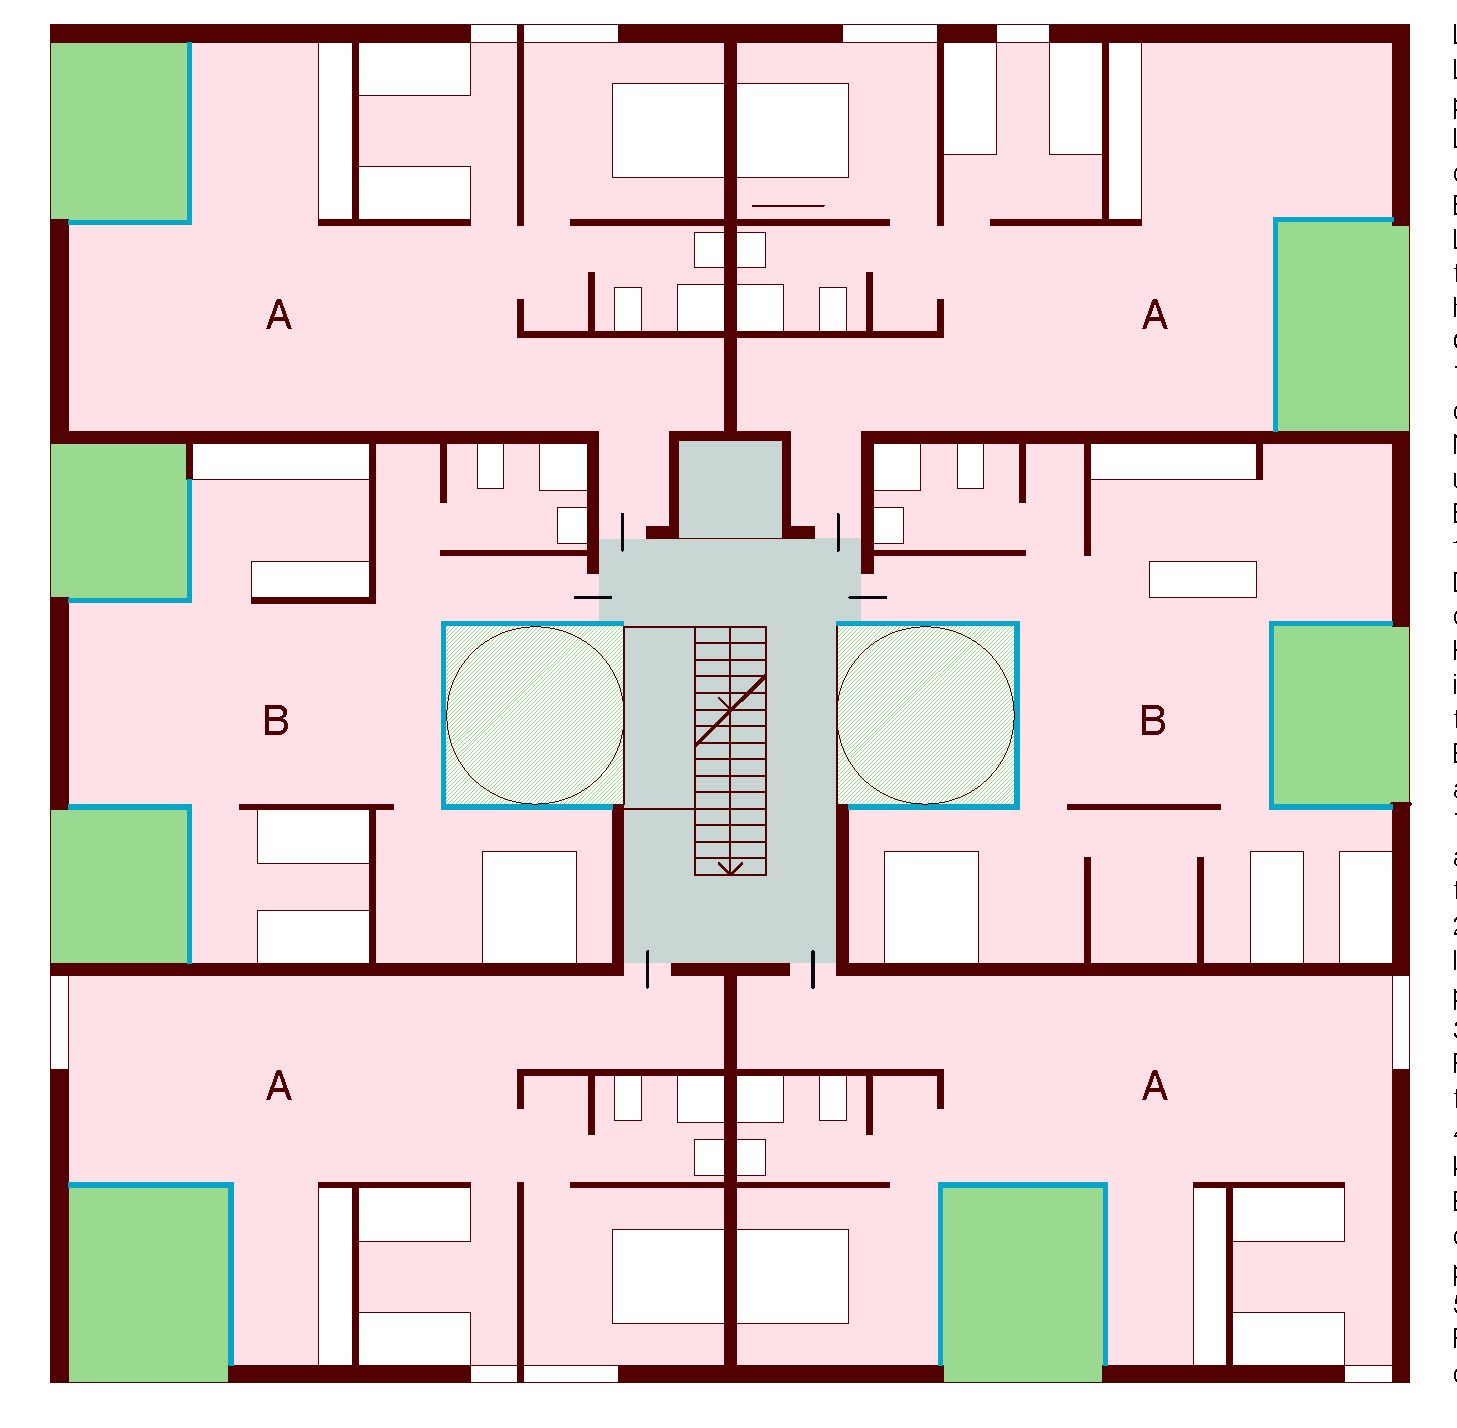
\includegraphics[width=0.55\textwidth]{figures/examples/inca_05.jpg}
\caption{One-shot reference image for Step~2, \code{inca\_05.jpg}, paired with
the expected JSON below.}
\label{fig:ex-agg}
\end{figure}

\noindent Expected JSON for the example image:

\begin{lstlisting}[style=prompt]
{
  "nodes": [
    {"node_id": 0, "type": "apartment", "label": "A", "door_position": [30, 22]},
    {"node_id": 1, "type": "apartment", "label": "A", "door_position": [70, 22]},
    {"node_id": 2, "type": "apartment", "label": "B", "door_position": [30, 50]},
    {"node_id": 3, "type": "apartment", "label": "B", "door_position": [70, 50]},
    {"node_id": 4, "type": "apartment", "label": "A", "door_position": [30, 78]},
    {"node_id": 5, "type": "apartment", "label": "A", "door_position": [70, 78]},
    {"node_id": 6, "type": "staircase", "label": null, "position": [50, 50]},
    {"node_id": 7, "type": "elevator",  "label": null, "position": [40, 50]},
    {"node_id": 8, "type": "elevator",  "label": null, "position": [60, 50]}
  ],
  "edges": [
    {"from_node_id": 0, "to_node_id": 6},
    {"from_node_id": 1, "to_node_id": 6},
    {"from_node_id": 2, "to_node_id": 6},
    {"from_node_id": 3, "to_node_id": 6},
    {"from_node_id": 4, "to_node_id": 6},
    {"from_node_id": 5, "to_node_id": 6},
    {"from_node_id": 6, "to_node_id": 7},
    {"from_node_id": 6, "to_node_id": 8}
  ]
}
\end{lstlisting}

% \section{Apartment Detailing (zero-shot)}
% \label{appendix:ex-details}

% No reference image is supplied. The prompt relies solely on the embedded
% Catalan/Spanish room-abbreviation dictionary and the typed JSON schema; the
% apartment under inspection is localised through the \code{\{apartment\_label\}},
% \code{\{x\}}, and \code{\{y\}} placeholders.

\section{Human-in-the-Loop Refinement (zero- to three-shot)}
\label{appendix:ex-review}

Architect-confirmed crops of the missed element --- up to three per type
(staircase, elevator) --- are loaded from the persistent visual-memory
directory \code{outputs/human\_review\_examples/} and prepended as reference
images, each captioned \textit{``Reference image: this is a STAIRCASE / ELEVATOR
as it appears in these floor plans.''} A plan reviewed before any crop has been
supplied receives no visual example (zero-shot); the count grows as the
architect contributes crops over successive sessions.


\chapter{Plan Examples}
\label{appendix:plan-examples}

This appendix shows the 2D extraction visualisations for the two floors used in the multi-floor assembly of Section~\ref{sec:exp-3d}: \textit{ibavi\_34}, the ground floor (\textit{planta baixa}), and \textit{ibavi\_35}, the first floor (\textit{planta primera}) of the same building. The two floors share an identical apartment layout--- ten units in a row served by a single staircase---which is what allows them to be stacked into a coherent multi-floor graph. Each figure places the original floor plan beside its 2D graph.

\begin{figure}[ht]
    \centering
    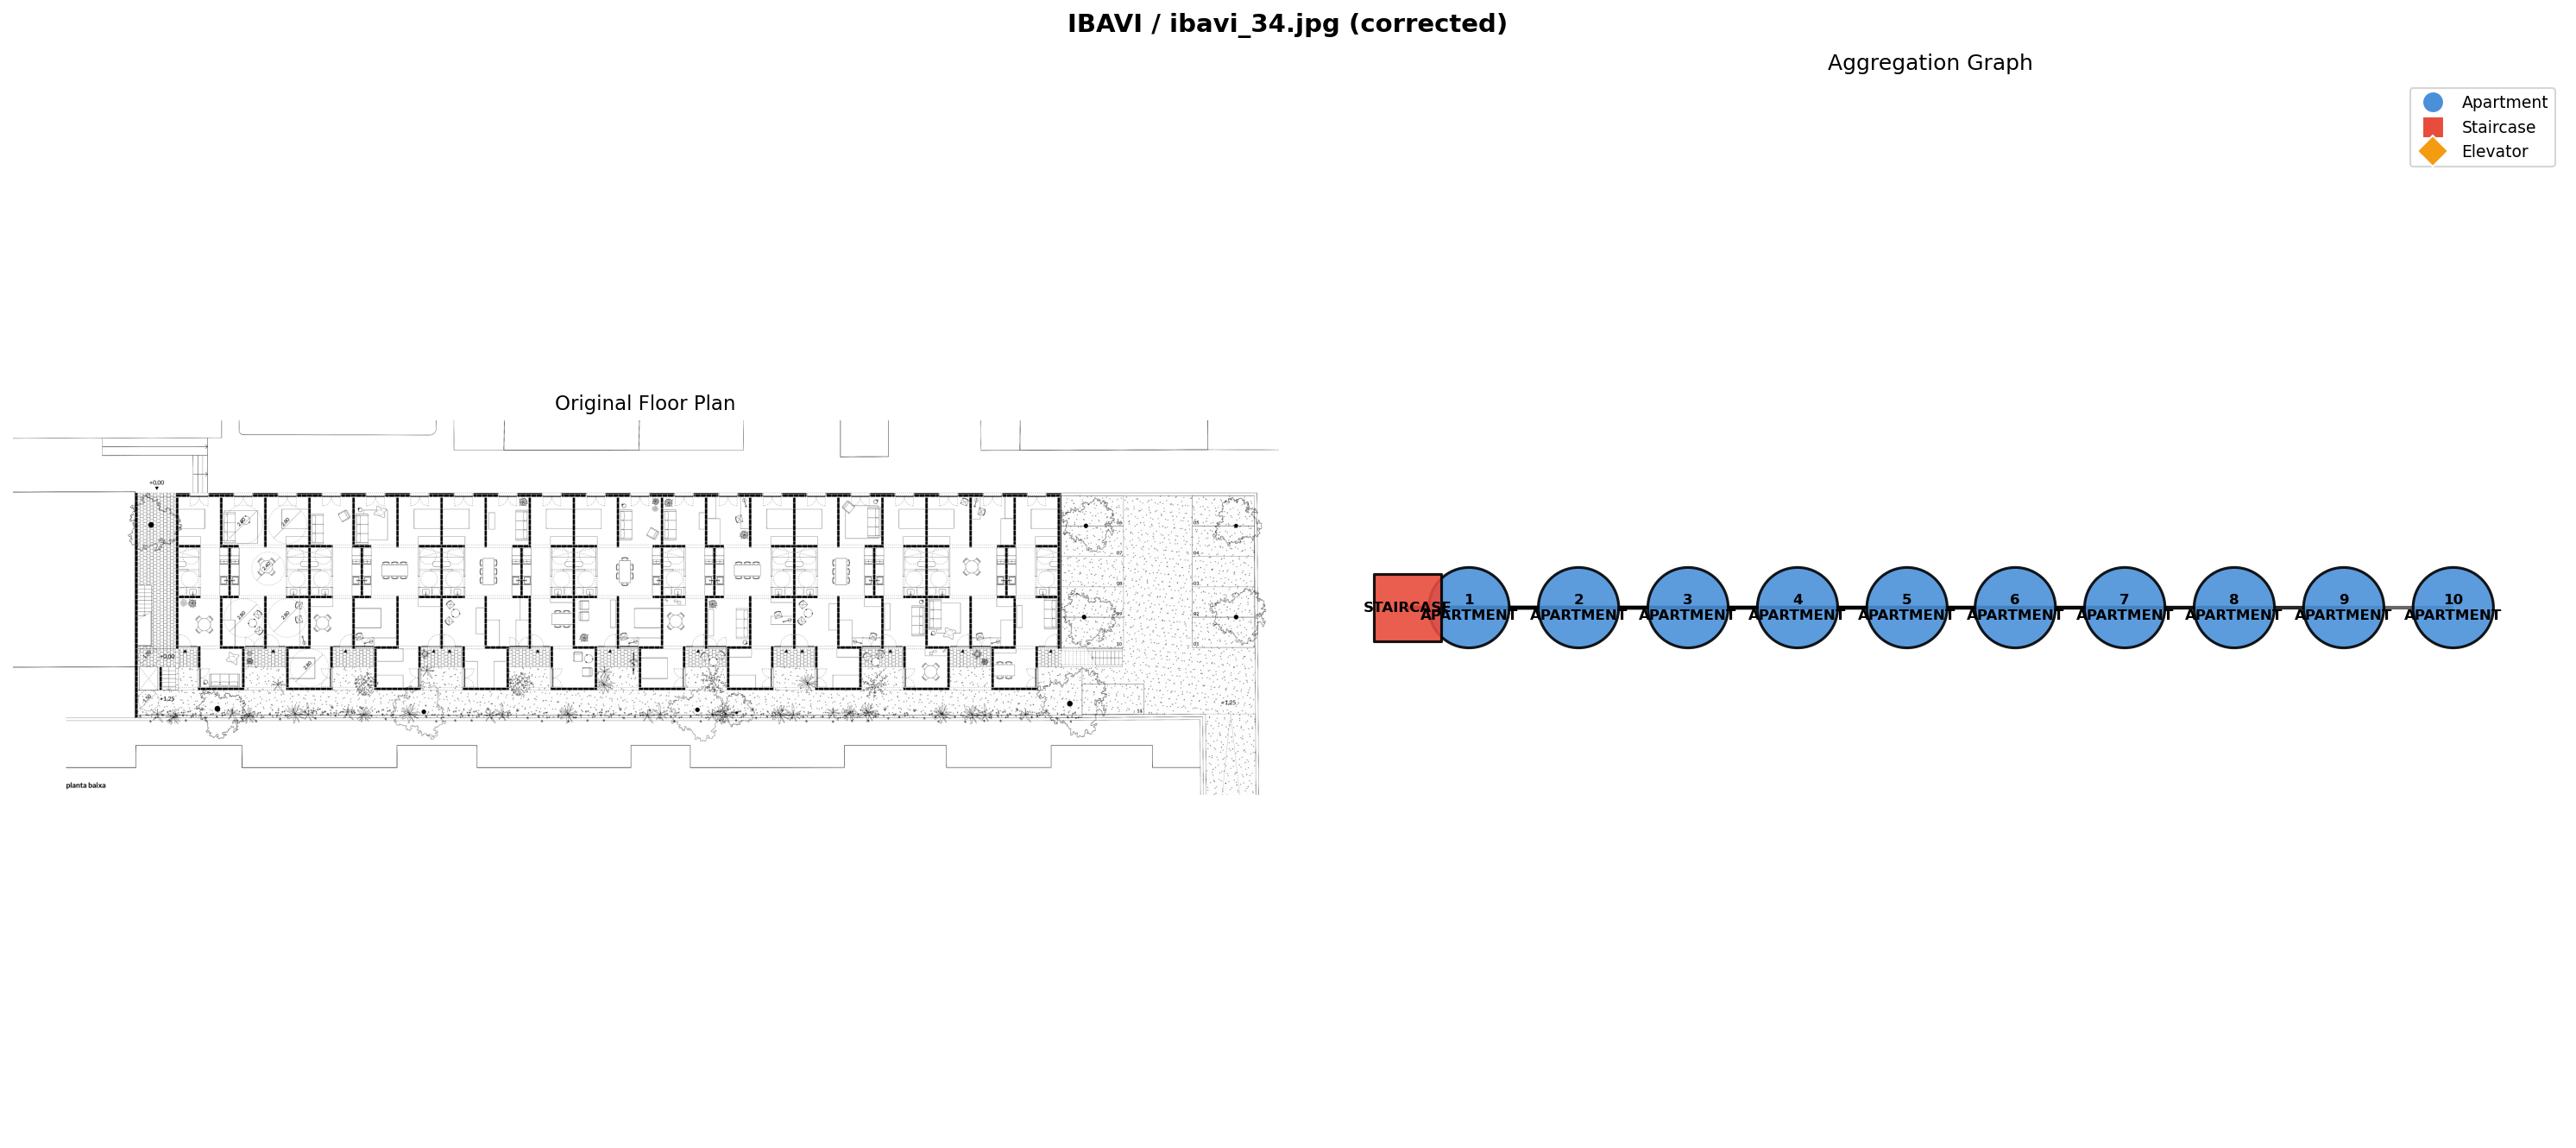
\includegraphics[width=0.7\linewidth]{figures/examples/ibavi_34_aggregation.png}
    \caption{\textit{ibavi\_34} (ground floor / \textit{planta baixa}): the original plan and its 2D graph of ten apartments in a row served by a single staircase.}
    \label{fig:ibavi_34}
\end{figure}

\begin{figure}[ht]
    \centering
    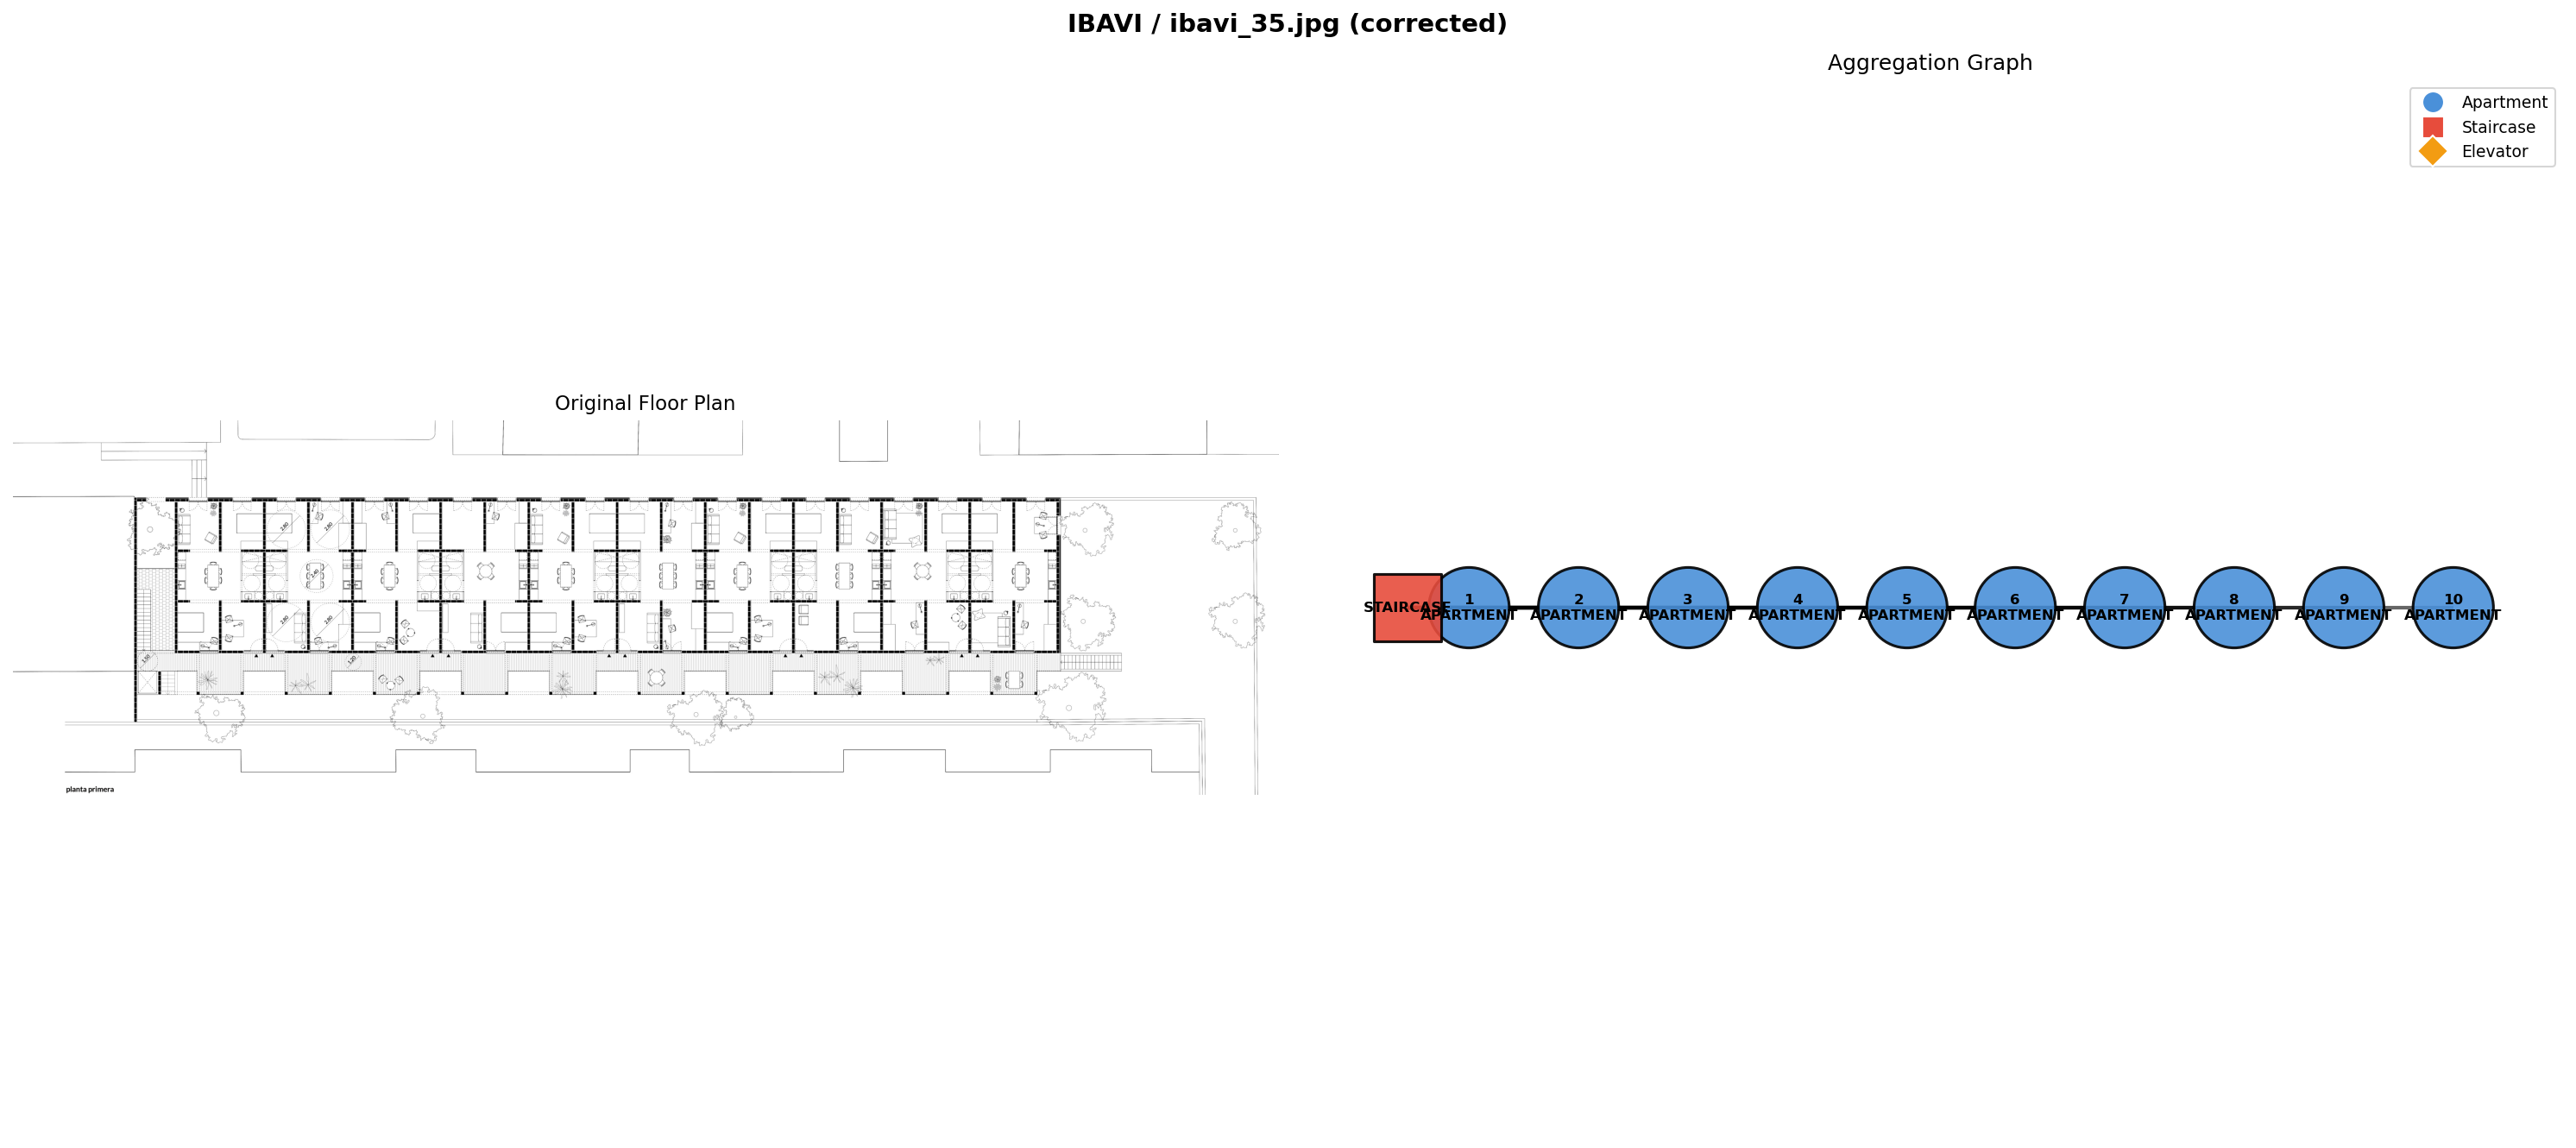
\includegraphics[width=0.7\linewidth]{figures/examples/ibavi_35_aggregation.png}
    \caption{\textit{ibavi\_35} (first floor / \textit{planta primera}): the same building's first floor, with an apartment layout identical to Figure~\ref{fig:ibavi_34}.}
    \label{fig:ibavi_35}
\end{figure}


% ============================================================
\chapter{Output Schema}
\label{appendix:json-schema}

This appendix documents the \textit{JSON} schema of the two artefacts produced by the pipeline, illustrated with the real output for \textit{ibavi\_9.jpg} (a linear corridor floor with six apartments served by one staircase and one elevator).

\section{2D Aggregation Graph}
\label{appendix:json-2d}

Each \code{\{name\}\_aggregation.json} file holds the per-image 2D access graph. The top level carries the source metadata and the captured \code{building\_analysis} reasoning trace. Each \emph{apartment} node embeds its room inventory---including
the per-node \code{spatial\_analysis} reasoning---under a \code{details} attribute, while \emph{staircase} and \emph{elevator} nodes carry only a centroid \code{position}. Edges encode the hub-and-spoke access topology. After validation, the object is annotated with \code{metadata} counts and a \code{flags} list (empty here, as the graph passes every check). The listing below shows the first two
apartment nodes in full and abbreviates the remaining four for brevity.

\begin{lstlisting}[style=prompt]
{
  "source_file": "ibavi_9.jpg",
  "dataset": "IBAVI",
  "type": "aggregation",
  "building_analysis": "Linear corridor layout with a central staircase and elevator core serving 6 apartments arranged in two rows on either side of the circulation spine.",
  "nodes": [
    {
      "node_id": 0,
      "type": "apartment",
      "label": "1A",
      "position": [85.0, 30.0],
      "details": {
        "num_bedrooms": 1,
        "num_bathrooms": 1,
        "num_kitchens": 1,
        "num_living_rooms": 1,
        "num_terraces": 1,
        "has_corridor": false,
        "total_rooms": 4,
        "room_labels": ["H", "EMC", "B", "Te"],
        "spatial_analysis": "Apartment 1A is located in the lower-right quadrant, bounded by the central corridor to the north, the building wall to the east, and the shared wall with apartment 1B to the south."
      }
    },
    {
      "node_id": 1,
      "type": "apartment",
      "label": "1B",
      "position": [85.0, 60.0],
      "details": {
        "num_bedrooms": 1, "num_bathrooms": 1, "num_kitchens": 1,
        "num_living_rooms": 1, "num_terraces": 1, "has_corridor": false,
        "total_rooms": 4, "room_labels": ["H", "EMC", "B", "Te"],
        "spatial_analysis": "Apartment 1B is bounded by the central corridor to the north, the building wall to the east, and the shared wall with apartment 1A to the south."
      }
    },
    /* ... apartment nodes 2-5 omitted (same structure) ... */
    {"node_id": 6, "type": "staircase", "label": "PB", "position": [50.0, 100.0]},
    {"node_id": 7, "type": "elevator",  "label": "PS", "position": [50.0, 130.0]}
  ],
  "edges": [
    {"from_node_id": 0, "to_node_id": 6},
    {"from_node_id": 1, "to_node_id": 6},
    {"from_node_id": 2, "to_node_id": 6},
    {"from_node_id": 3, "to_node_id": 6},
    {"from_node_id": 4, "to_node_id": 6},
    {"from_node_id": 5, "to_node_id": 6},
    {"from_node_id": 6, "to_node_id": 7}
  ],
  "metadata": {
    "num_apartments": 6, "num_staircases": 1, "num_elevators": 1,
    "num_edges": 7, "apartments_with_details": 6
  },
  "flags": []
}
\end{lstlisting}

\section{3D Building Graph}
\label{appendix:json-3d}

Each \code{\{name\}\_3d.json} file stacks the 2D floor into an $N$-floor building (here $N=3$). Node identifiers are globalised as
$\mathrm{id}_{3D} = f \times 10^{6} + \mathrm{id}_{2D}$, so the floor index is recoverable, and each node gains a \code{floor} field. Edges are tagged \code{horizontal} (within a floor, carrying the floor index) or \code{vertical} (between consecutive floors, carrying the \code{via} connector type). The listing abbreviates the node and edge lists, showing one staircase per floor and one edge of each type.

\begin{lstlisting}[style=prompt]
{
  "source_file": "ibavi_9.jpg",
  "dataset": "IBAVI",
  "type": "building_3d",
  "n_floors": 3,
  "nodes": [
    {
      "node_id": 0,
      "floor": 0,
      "type": "apartment",
      "label": "1A",
      "position": [
        85.0,
        30.0
      ],
      "details": {
        "num_bedrooms": 1,
        "num_bathrooms": 1,
        "num_kitchens": 1,
        "num_living_rooms": 1,
        "num_terraces": 1,
        "has_corridor": false,
        "total_rooms": 4,
        "room_labels": [
          "H",
          "EMC",
          "B",
          "Te"
        ],
        "spatial_analysis": "Apartment 1A is located in the lower-right quadrant, bounded by the central corridor to the north, the building wall to the east, and the shared wall with apartment 1B to the south."
      }
    },
    {
      "node_id": 1,
      "floor": 0,
      "type": "apartment",
      "label": "1B",
      "position": [
        85.0,
        60.0
      ],
      "details": {
        "num_bedrooms": 1,
        "num_bathrooms": 1,
        "num_kitchens": 1,
        "num_living_rooms": 1,
        "num_terraces": 1,
        "has_corridor": false,
        "total_rooms": 4,
        "room_labels": [
          "H",
          "EMC",
          "B",
          "Te"
        ],
        "spatial_analysis": "Apartment 1B is located in the lower-right quadrant of the plan, bounded by the central corridor to the north, the building wall to the east, and the shared wall with apartment 1A to the south."
      }
    },
    {
      "node_id": 2,
      "floor": 0,
      "type": "apartment",
      "label": "2A",
      "position": [
        85.0,
        90.0
      ],
      "details": {
        "num_bedrooms": 2,
        "num_bathrooms": 1,
        "num_kitchens": 1,
        "num_living_rooms": 1,
        "num_terraces": 1,
        "has_corridor": false,
        "total_rooms": 5,
        "room_labels": [
          "H",
          "H",
          "EMC",
          "B",
          "Te"
        ],
        "spatial_analysis": "Apartment 2A is located in the upper-middle section of the plan, bounded by the central corridor to the south, the building wall to the east, and the corridor to the west."
      }
    },
    {
      "node_id": 3,
      "floor": 0,
      "type": "apartment",
      "label": "2A",
      "position": [
        85.0,
        120.0
      ],
      "details": {
        "num_bedrooms": 2,
        "num_bathrooms": 1,
        "num_kitchens": 1,
        "num_living_rooms": 1,
        "num_terraces": 1,
        "has_corridor": false,
        "total_rooms": 5,
        "room_labels": [
          "H",
          "H",
          "EMC",
          "B",
          "Te"
        ],
        "spatial_analysis": "Apartment 2A is located in the upper-middle section of the plan, bounded by the central corridor to the south and the building wall to the east and west."
      }
    },
    {
      "node_id": 4,
      "floor": 0,
      "type": "apartment",
      "label": "2B",
      "position": [
        85.0,
        150.0
      ],
      "details": {
        "num_bedrooms": 2,
        "num_bathrooms": 1,
        "num_kitchens": 1,
        "num_living_rooms": 1,
        "num_terraces": 1,
        "has_corridor": false,
        "total_rooms": 5,
        "room_labels": [
          "H",
          "H1",
          "EMC",
          "B",
          "Te"
        ],
        "spatial_analysis": "Apartment 2B is located in the lower-left section of the plan, bounded by the central corridor to the north, the building wall to the west, and the shared wall with apartment 2A to the east."
      }
    },
    {
      "node_id": 5,
      "floor": 0,
      "type": "apartment",
      "label": "HA",
      "position": [
        85.0,
        180.0
      ],
      "details": {
        "num_bedrooms": 1,
        "num_bathrooms": 1,
        "num_kitchens": 1,
        "num_living_rooms": 1,
        "num_terraces": 1,
        "has_corridor": false,
        "total_rooms": 4,
        "room_labels": [
          "H",
          "EMC",
          "B",
          "Te"
        ],
        "spatial_analysis": "Apartment HA is located in the lower-right quadrant, bounded by the central corridor to the north, the building wall to the east, and the shared wall with apartment 1B to the south."
      }
    },
    {
      "node_id": 6,
      "floor": 0,
      "type": "staircase",
      "label": "PB",
      "position": [
        50.0,
        100.0
      ]
    },
    {
      "node_id": 7,
      "floor": 0,
      "type": "elevator",
      "label": "PS",
      "position": [
        50.0,
        130.0
      ]
    },
    {
      "node_id": 1000000,
      "floor": 1,
      "type": "apartment",
      "label": "1A",
      "position": [
        85.0,
        30.0
      ],
      "details": {
        "num_bedrooms": 1,
        "num_bathrooms": 1,
        "num_kitchens": 1,
        "num_living_rooms": 1,
        "num_terraces": 1,
        "has_corridor": false,
        "total_rooms": 4,
        "room_labels": [
          "H",
          "EMC",
          "B",
          "Te"
        ],
        "spatial_analysis": "Apartment 1A is located in the lower-right quadrant, bounded by the central corridor to the north, the building wall to the east, and the shared wall with apartment 1B to the south."
      }
    },
    {
      "node_id": 1000001,
      "floor": 1,
      "type": "apartment",
      "label": "1B",
      "position": [
        85.0,
        60.0
      ],
      "details": {
        "num_bedrooms": 1,
        "num_bathrooms": 1,
        "num_kitchens": 1,
        "num_living_rooms": 1,
        "num_terraces": 1,
        "has_corridor": false,
        "total_rooms": 4,
        "room_labels": [
          "H",
          "EMC",
          "B",
          "Te"
        ],
        "spatial_analysis": "Apartment 1B is located in the lower-right quadrant of the plan, bounded by the central corridor to the north, the building wall to the east, and the shared wall with apartment 1A to the south."
      }
    },
    {
      "node_id": 1000002,
      "floor": 1,
      "type": "apartment",
      "label": "2A",
      "position": [
        85.0,
        90.0
      ],
      "details": {
        "num_bedrooms": 2,
        "num_bathrooms": 1,
        "num_kitchens": 1,
        "num_living_rooms": 1,
        "num_terraces": 1,
        "has_corridor": false,
        "total_rooms": 5,
        "room_labels": [
          "H",
          "H",
          "EMC",
          "B",
          "Te"
        ],
        "spatial_analysis": "Apartment 2A is located in the upper-middle section of the plan, bounded by the central corridor to the south, the building wall to the east, and the corridor to the west."
      }
    },
    {
      "node_id": 1000003,
      "floor": 1,
      "type": "apartment",
      "label": "2A",
      "position": [
        85.0,
        120.0
      ],
      "details": {
        "num_bedrooms": 2,
        "num_bathrooms": 1,
        "num_kitchens": 1,
        "num_living_rooms": 1,
        "num_terraces": 1,
        "has_corridor": false,
        "total_rooms": 5,
        "room_labels": [
          "H",
          "H",
          "EMC",
          "B",
          "Te"
        ],
        "spatial_analysis": "Apartment 2A is located in the upper-middle section of the plan, bounded by the central corridor to the south and the building wall to the east and west."
      }
    },
    {
      "node_id": 1000004,
      "floor": 1,
      "type": "apartment",
      "label": "2B",
      "position": [
        85.0,
        150.0
      ],
      "details": {
        "num_bedrooms": 2,
        "num_bathrooms": 1,
        "num_kitchens": 1,
        "num_living_rooms": 1,
        "num_terraces": 1,
        "has_corridor": false,
        "total_rooms": 5,
        "room_labels": [
          "H",
          "H1",
          "EMC",
          "B",
          "Te"
        ],
        "spatial_analysis": "Apartment 2B is located in the lower-left section of the plan, bounded by the central corridor to the north, the building wall to the west, and the shared wall with apartment 2A to the east."
      }
    },
    {
      "node_id": 1000005,
      "floor": 1,
      "type": "apartment",
      "label": "HA",
      "position": [
        85.0,
        180.0
      ],
      "details": {
        "num_bedrooms": 1,
        "num_bathrooms": 1,
        "num_kitchens": 1,
        "num_living_rooms": 1,
        "num_terraces": 1,
        "has_corridor": false,
        "total_rooms": 4,
        "room_labels": [
          "H",
          "EMC",
          "B",
          "Te"
        ],
        "spatial_analysis": "Apartment HA is located in the lower-right quadrant, bounded by the central corridor to the north, the building wall to the east, and the shared wall with apartment 1B to the south."
      }
    },
    {
      "node_id": 1000006,
      "floor": 1,
      "type": "staircase",
      "label": "PB",
      "position": [
        50.0,
        100.0
      ]
    },
    {
      "node_id": 1000007,
      "floor": 1,
      "type": "elevator",
      "label": "PS",
      "position": [
        50.0,
        130.0
      ]
    },
    {
      "node_id": 2000000,
      "floor": 2,
      "type": "apartment",
      "label": "1A",
      "position": [
        85.0,
        30.0
      ],
      "details": {
        "num_bedrooms": 1,
        "num_bathrooms": 1,
        "num_kitchens": 1,
        "num_living_rooms": 1,
        "num_terraces": 1,
        "has_corridor": false,
        "total_rooms": 4,
        "room_labels": [
          "H",
          "EMC",
          "B",
          "Te"
        ],
        "spatial_analysis": "Apartment 1A is located in the lower-right quadrant, bounded by the central corridor to the north, the building wall to the east, and the shared wall with apartment 1B to the south."
      }
    },
    {
      "node_id": 2000001,
      "floor": 2,
      "type": "apartment",
      "label": "1B",
      "position": [
        85.0,
        60.0
      ],
      "details": {
        "num_bedrooms": 1,
        "num_bathrooms": 1,
        "num_kitchens": 1,
        "num_living_rooms": 1,
        "num_terraces": 1,
        "has_corridor": false,
        "total_rooms": 4,
        "room_labels": [
          "H",
          "EMC",
          "B",
          "Te"
        ],
        "spatial_analysis": "Apartment 1B is located in the lower-right quadrant of the plan, bounded by the central corridor to the north, the building wall to the east, and the shared wall with apartment 1A to the south."
      }
    },
    {
      "node_id": 2000002,
      "floor": 2,
      "type": "apartment",
      "label": "2A",
      "position": [
        85.0,
        90.0
      ],
      "details": {
        "num_bedrooms": 2,
        "num_bathrooms": 1,
        "num_kitchens": 1,
        "num_living_rooms": 1,
        "num_terraces": 1,
        "has_corridor": false,
        "total_rooms": 5,
        "room_labels": [
          "H",
          "H",
          "EMC",
          "B",
          "Te"
        ],
        "spatial_analysis": "Apartment 2A is located in the upper-middle section of the plan, bounded by the central corridor to the south, the building wall to the east, and the corridor to the west."
      }
    },
    {
      "node_id": 2000003,
      "floor": 2,
      "type": "apartment",
      "label": "2A",
      "position": [
        85.0,
        120.0
      ],
      "details": {
        "num_bedrooms": 2,
        "num_bathrooms": 1,
        "num_kitchens": 1,
        "num_living_rooms": 1,
        "num_terraces": 1,
        "has_corridor": false,
        "total_rooms": 5,
        "room_labels": [
          "H",
          "H",
          "EMC",
          "B",
          "Te"
        ],
        "spatial_analysis": "Apartment 2A is located in the upper-middle section of the plan, bounded by the central corridor to the south and the building wall to the east and west."
      }
    },
    {
      "node_id": 2000004,
      "floor": 2,
      "type": "apartment",
      "label": "2B",
      "position": [
        85.0,
        150.0
      ],
      "details": {
        "num_bedrooms": 2,
        "num_bathrooms": 1,
        "num_kitchens": 1,
        "num_living_rooms": 1,
        "num_terraces": 1,
        "has_corridor": false,
        "total_rooms": 5,
        "room_labels": [
          "H",
          "H1",
          "EMC",
          "B",
          "Te"
        ],
        "spatial_analysis": "Apartment 2B is located in the lower-left section of the plan, bounded by the central corridor to the north, the building wall to the west, and the shared wall with apartment 2A to the east."
      }
    },
    {
      "node_id": 2000005,
      "floor": 2,
      "type": "apartment",
      "label": "HA",
      "position": [
        85.0,
        180.0
      ],
      "details": {
        "num_bedrooms": 1,
        "num_bathrooms": 1,
        "num_kitchens": 1,
        "num_living_rooms": 1,
        "num_terraces": 1,
        "has_corridor": false,
        "total_rooms": 4,
        "room_labels": [
          "H",
          "EMC",
          "B",
          "Te"
        ],
        "spatial_analysis": "Apartment HA is located in the lower-right quadrant, bounded by the central corridor to the north, the building wall to the east, and the shared wall with apartment 1B to the south."
      }
    },
    {
      "node_id": 2000006,
      "floor": 2,
      "type": "staircase",
      "label": "PB",
      "position": [
        50.0,
        100.0
      ]
    },
    {
      "node_id": 2000007,
      "floor": 2,
      "type": "elevator",
      "label": "PS",
      "position": [
        50.0,
        130.0
      ]
    }
  ],
  "edges": [
    {
      "from_node_id": 0,
      "to_node_id": 6,
      "edge_type": "horizontal",
      "floor": 0
    },
    {
      "from_node_id": 1,
      "to_node_id": 6,
      "edge_type": "horizontal",
      "floor": 0
    },
    {
      "from_node_id": 2,
      "to_node_id": 6,
      "edge_type": "horizontal",
      "floor": 0
    },
    {
      "from_node_id": 3,
      "to_node_id": 6,
      "edge_type": "horizontal",
      "floor": 0
    },
    {
      "from_node_id": 4,
      "to_node_id": 6,
      "edge_type": "horizontal",
      "floor": 0
    },
    {
      "from_node_id": 5,
      "to_node_id": 6,
      "edge_type": "horizontal",
      "floor": 0
    },
    {
      "from_node_id": 6,
      "to_node_id": 7,
      "edge_type": "horizontal",
      "floor": 0
    },
    {
      "from_node_id": 1000000,
      "to_node_id": 1000006,
      "edge_type": "horizontal",
      "floor": 1
    },
    {
      "from_node_id": 1000001,
      "to_node_id": 1000006,
      "edge_type": "horizontal",
      "floor": 1
    },
    {
      "from_node_id": 1000002,
      "to_node_id": 1000006,
      "edge_type": "horizontal",
      "floor": 1
    },
    {
      "from_node_id": 1000003,
      "to_node_id": 1000006,
      "edge_type": "horizontal",
      "floor": 1
    },
    {
      "from_node_id": 1000004,
      "to_node_id": 1000006,
      "edge_type": "horizontal",
      "floor": 1
    },
    {
      "from_node_id": 1000005,
      "to_node_id": 1000006,
      "edge_type": "horizontal",
      "floor": 1
    },
    {
      "from_node_id": 1000006,
      "to_node_id": 1000007,
      "edge_type": "horizontal",
      "floor": 1
    },
    {
      "from_node_id": 2000000,
      "to_node_id": 2000006,
      "edge_type": "horizontal",
      "floor": 2
    },
    {
      "from_node_id": 2000001,
      "to_node_id": 2000006,
      "edge_type": "horizontal",
      "floor": 2
    },
    {
      "from_node_id": 2000002,
      "to_node_id": 2000006,
      "edge_type": "horizontal",
      "floor": 2
    },
    {
      "from_node_id": 2000003,
      "to_node_id": 2000006,
      "edge_type": "horizontal",
      "floor": 2
    },
    {
      "from_node_id": 2000004,
      "to_node_id": 2000006,
      "edge_type": "horizontal",
      "floor": 2
    },
    {
      "from_node_id": 2000005,
      "to_node_id": 2000006,
      "edge_type": "horizontal",
      "floor": 2
    },
    {
      "from_node_id": 2000006,
      "to_node_id": 2000007,
      "edge_type": "horizontal",
      "floor": 2
    },
    {
      "from_node_id": 6,
      "to_node_id": 1000006,
      "edge_type": "vertical",
      "via": "staircase"
    },
    {
      "from_node_id": 7,
      "to_node_id": 1000007,
      "edge_type": "vertical",
      "via": "elevator"
    },
    {
      "from_node_id": 1000006,
      "to_node_id": 2000006,
      "edge_type": "vertical",
      "via": "staircase"
    },
    {
      "from_node_id": 1000007,
      "to_node_id": 2000007,
      "edge_type": "vertical",
      "via": "elevator"
    }
  ],
  "metadata": {
    "num_apartments": 18,
    "num_staircases": 3,
    "num_elevators": 3,
    "num_horizontal_edges": 21,
    "num_vertical_edges": 4
  },
  "flags": []
}
\end{lstlisting}

\end{appendices}





\end{document}
